\documentclass[a4paper,pra,twocolumn,10pt,aps,longbibliography,nobalancelastpage]{revtex4-1}

\usepackage{geometry}
\usepackage{graphicx}
\usepackage{amsmath}
\usepackage{listings}
\usepackage{units}
\usepackage{balance}
\usepackage{float}
\usepackage{capt-of}
\usepackage{xfrac}
\graphicspath{{images/}}

\geometry{
 	a4paper,
 	total={170mm,257mm},
 	left=10mm,
 	right=10mm,
 	top=20mm,
 	bottom=20mm
} 
\setlength{\intextsep}{1.0pt plus 0.5pt minus 0.5pt}

\begin{document}
\title{Machine Learning For Computer Vision: Random Decision Forest}
\author{Sagar Patel, CID: 00842688, and Pranav Malhotra, CID: 00823617}
\date{14th March 2017}

\maketitle

\section{Train Decision Forest}\label{sec:train}

\subsection{Bootstrap Aggregating}
Using Bootstrap Aggregating (Bagging), multiple data subsets are generated by uniformly selecting data points from the training set with replacement. This introduces some randomness into the
training data used to grow each tree in the random decision forest. The in-built matlab function \texttt{randsample} is used to generate each dataset. 

\begin{figure}[H]
	\centering
    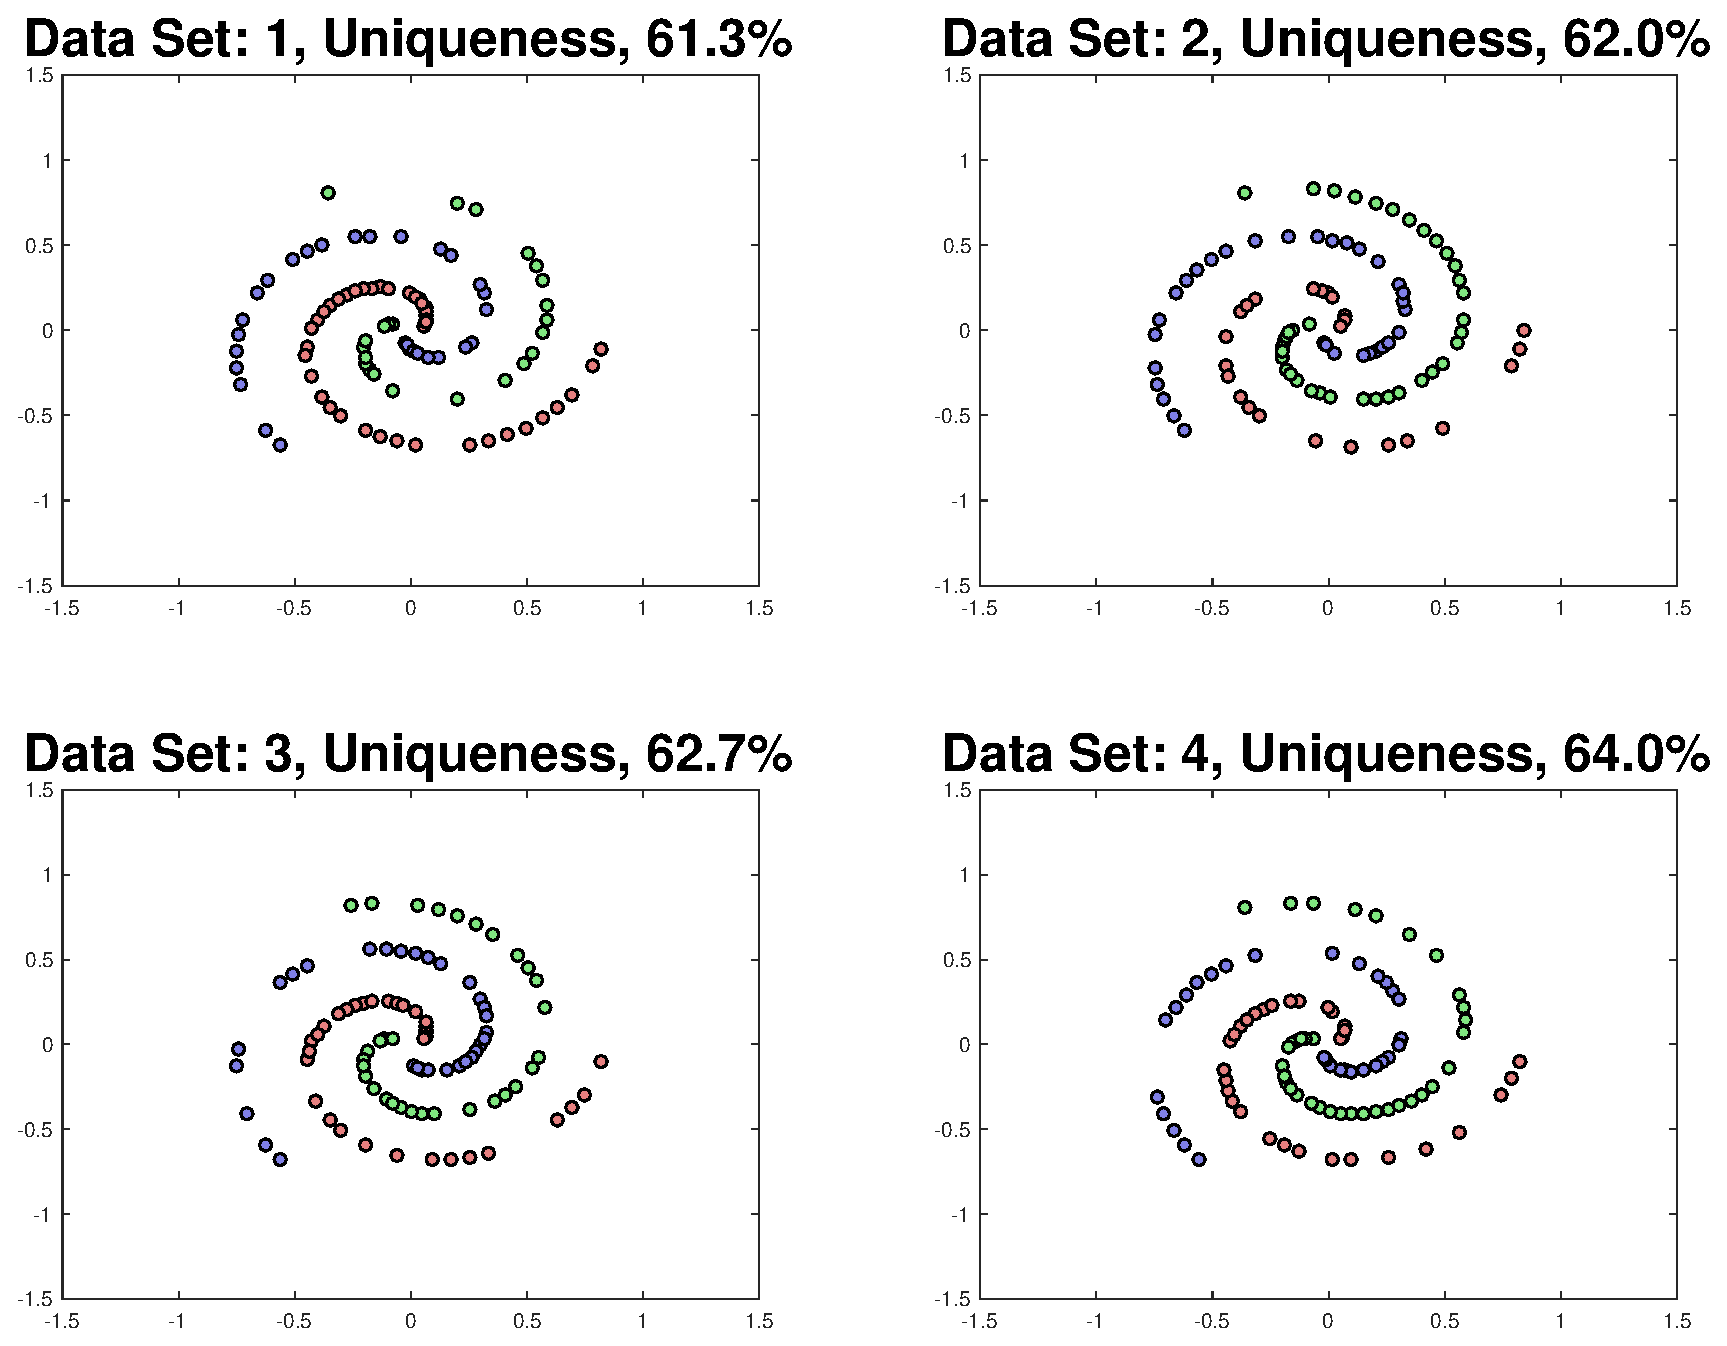
\includegraphics[width=0.60\columnwidth]{boot_strap}
    \caption{Overview of spectral subtraction process}
    \label{fig:boot_strap}
\end{figure}

The resulting data subsets have been visualized in Figure \ref{fig:boot_strap}. Each data subset has 150 points however the spirals are not complete. This is due to the fact that samples are drawn from the training dataset with replacement. The amount of uniqueness in within each subset is presented in Figure \ref{fig:boot_strap} as well.  Ideally, as the size of our training dataset increases, the uniqueness should approach $63.3\%$. The finite size of our training dataset results in uniqueness values spread around the ideal. The table below shows the probability distributions of each class within each data subset. The roughly equal distributions corroborate the fact that sampling was performed uniformly.

\begin{table}[H]
\centering
\begin{tabular}{|c|c|}
\hline
Dataset Index & Class Probabilities 		\\ \hline
1             & $[0.3733, 0.2733, 0.3533]$  	\\ \hline
2             & $[0.2800, 0.3667, 0.3533]$  	\\ \hline
3             & $[0.3333, 0.3200, 0.3467]$ 	\\ \hline
4             & $[0.3467, 0.3133, 0.3400]$  	\\ \hline
\end{tabular}
\end{table}

\subsection{Split Function}

The first step in the training of the decision forest is to develop the weak-learner functions that will be used to split the data at each node of the tree. Multiple weak-learner functions were implemented, namely axis-aligned, two-pixel, linear, quadratic and cubic.

\begin{align}
h(\textbf{v}, \theta) = [&a_1x_1^2+a_2x_2^2+a_3x_1x_2+a_4x_1+a_5x_2>\tau] \label{eq:quad_split} \\
h(\textbf{v}, \theta) = [&a_1x_1^3+a_2x_2^3+a_3x_1^2x_2+a_4x_1x_2^2+a_5x_1^2 \nonumber\\
&+a_6x_2^2+a_7x_1x_2+a_8x_1+a_9x_2>\tau] \label{eq:cubic_split}
\end{align}

Note that the axis-aligned, two-pixel and linear learners have the general form presented in the lecture notes whereas the quadratic and cubic split functions have the form expressed in (\ref{eq:quad_split}) and (\ref{eq:cubic_split}) respectively. The quadratic and cubic learners are non-linear in 2-dimensional space but are implemented by transforming the data and using linear separators.

\begin{figure}[H]
	\centering
    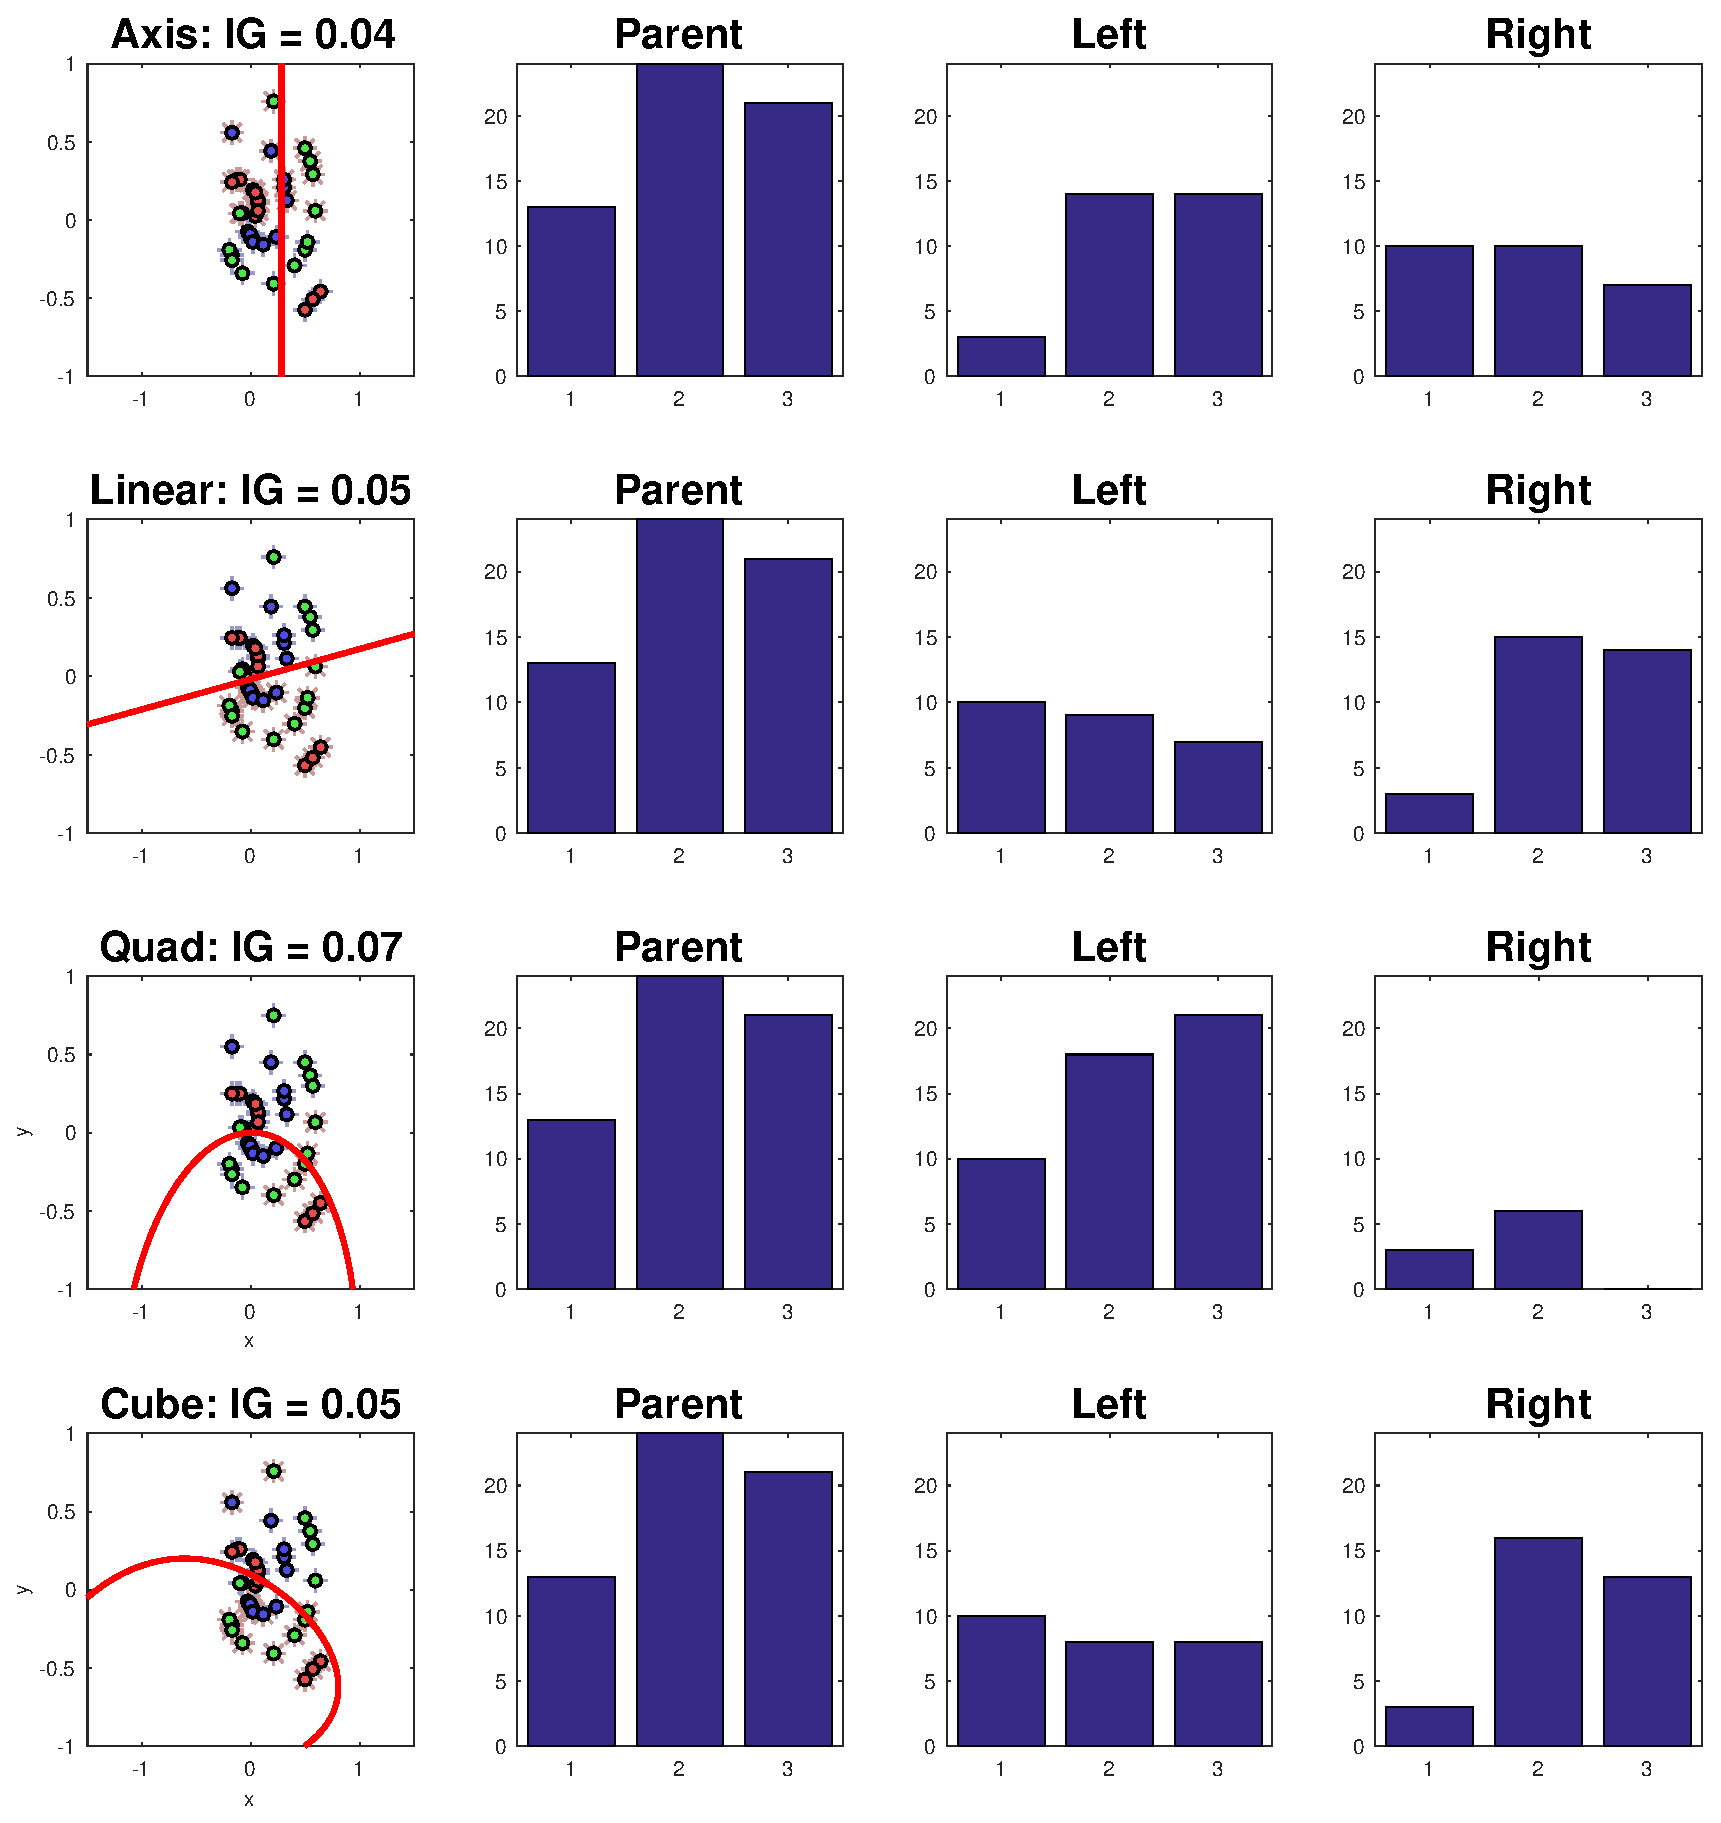
\includegraphics[width=0.60\columnwidth]{split_function_visualitions_1}
    \caption{Overview of spectral subtraction process}
    \label{fig:ex_func}
\end{figure}

Example split functions for all learners, except the two-pixel test are presented in Figure \ref{fig:ex_func}. The two-pixel test does not perform well with 2-dimensional data. The results are indicative of the fact that a stronger class of learner functions does not necessarily translate into a greater information gain; this is especially true if the number of split functions over which optimization is performed is small.

\begin{figure}[H]
	\centering
    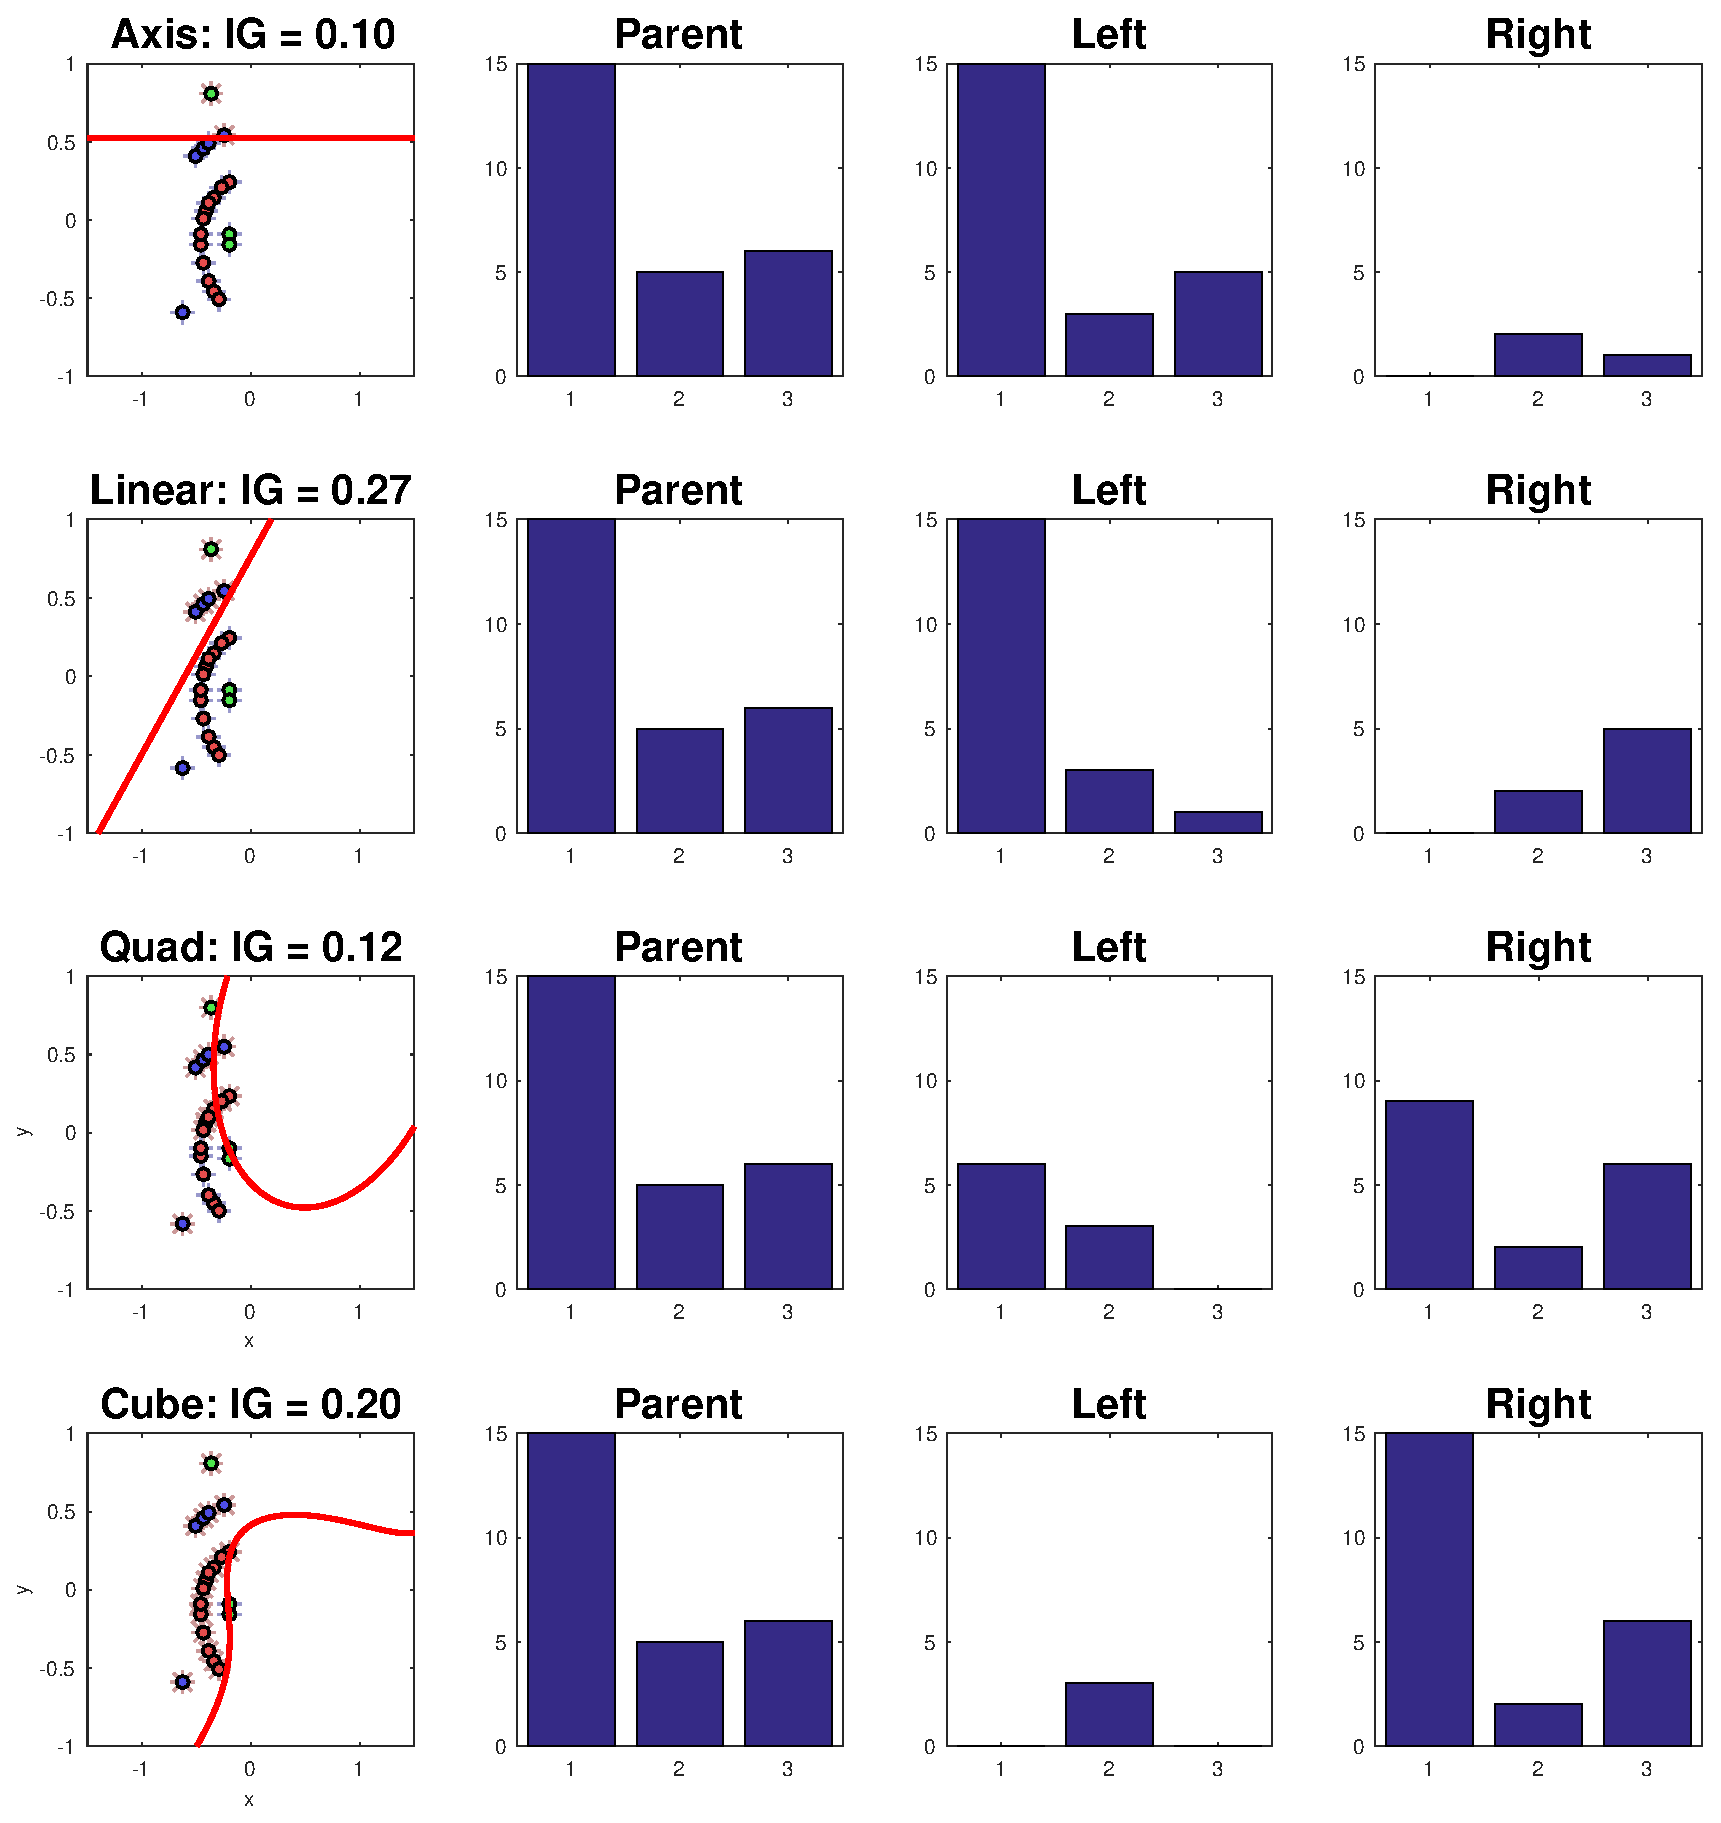
\includegraphics[width=0.60\columnwidth]{split_function_visualitions_3}
    \caption{Overview of spectral subtraction process}
    \label{fig:learners_2}
\end{figure}

The graph in Figure \ref{fig:learners_2} shows what happens when a strong learning class is trained on a small number of data points. Observe the split function obtained for the quadratic and cubic learners; \textbf{there is clear over-fitting of the data.} This is completely in line with the results obtained from Vapnik--Chervonenkis (VC) theory. Quadratic and cubic functions have a larger VC dimension and trained on a small number of points, these classes overfit training data and do not generalize well. The random forest algorithm provides a mechanism, the committee machine, to combat over-fitting in each individual tree. As such, in the next section, it should be noted that if strong non-linear learners are used, the number of trees should also be increased to achieve the same performance as a weak-learner. 

By simply analyzing Figure \ref{fig:ex_func} and \ref{fig:learners_2}, the advantages of using a stronger learning class are not clear. For this, we have to increase \texttt{param.splitNum}. Figure \ref{fig:learners_3} makes it clear that stronger learning classes are able to split the data more efficiently and obtain a higher information gain. The discriminating power of the learning classes is not obvious when the number of split functions tested is small however increasing \texttt{param.splitNum} clearly highlights the intrinsic discriminating power of each weak-learner. 

\begin{figure}[H]
	\centering
    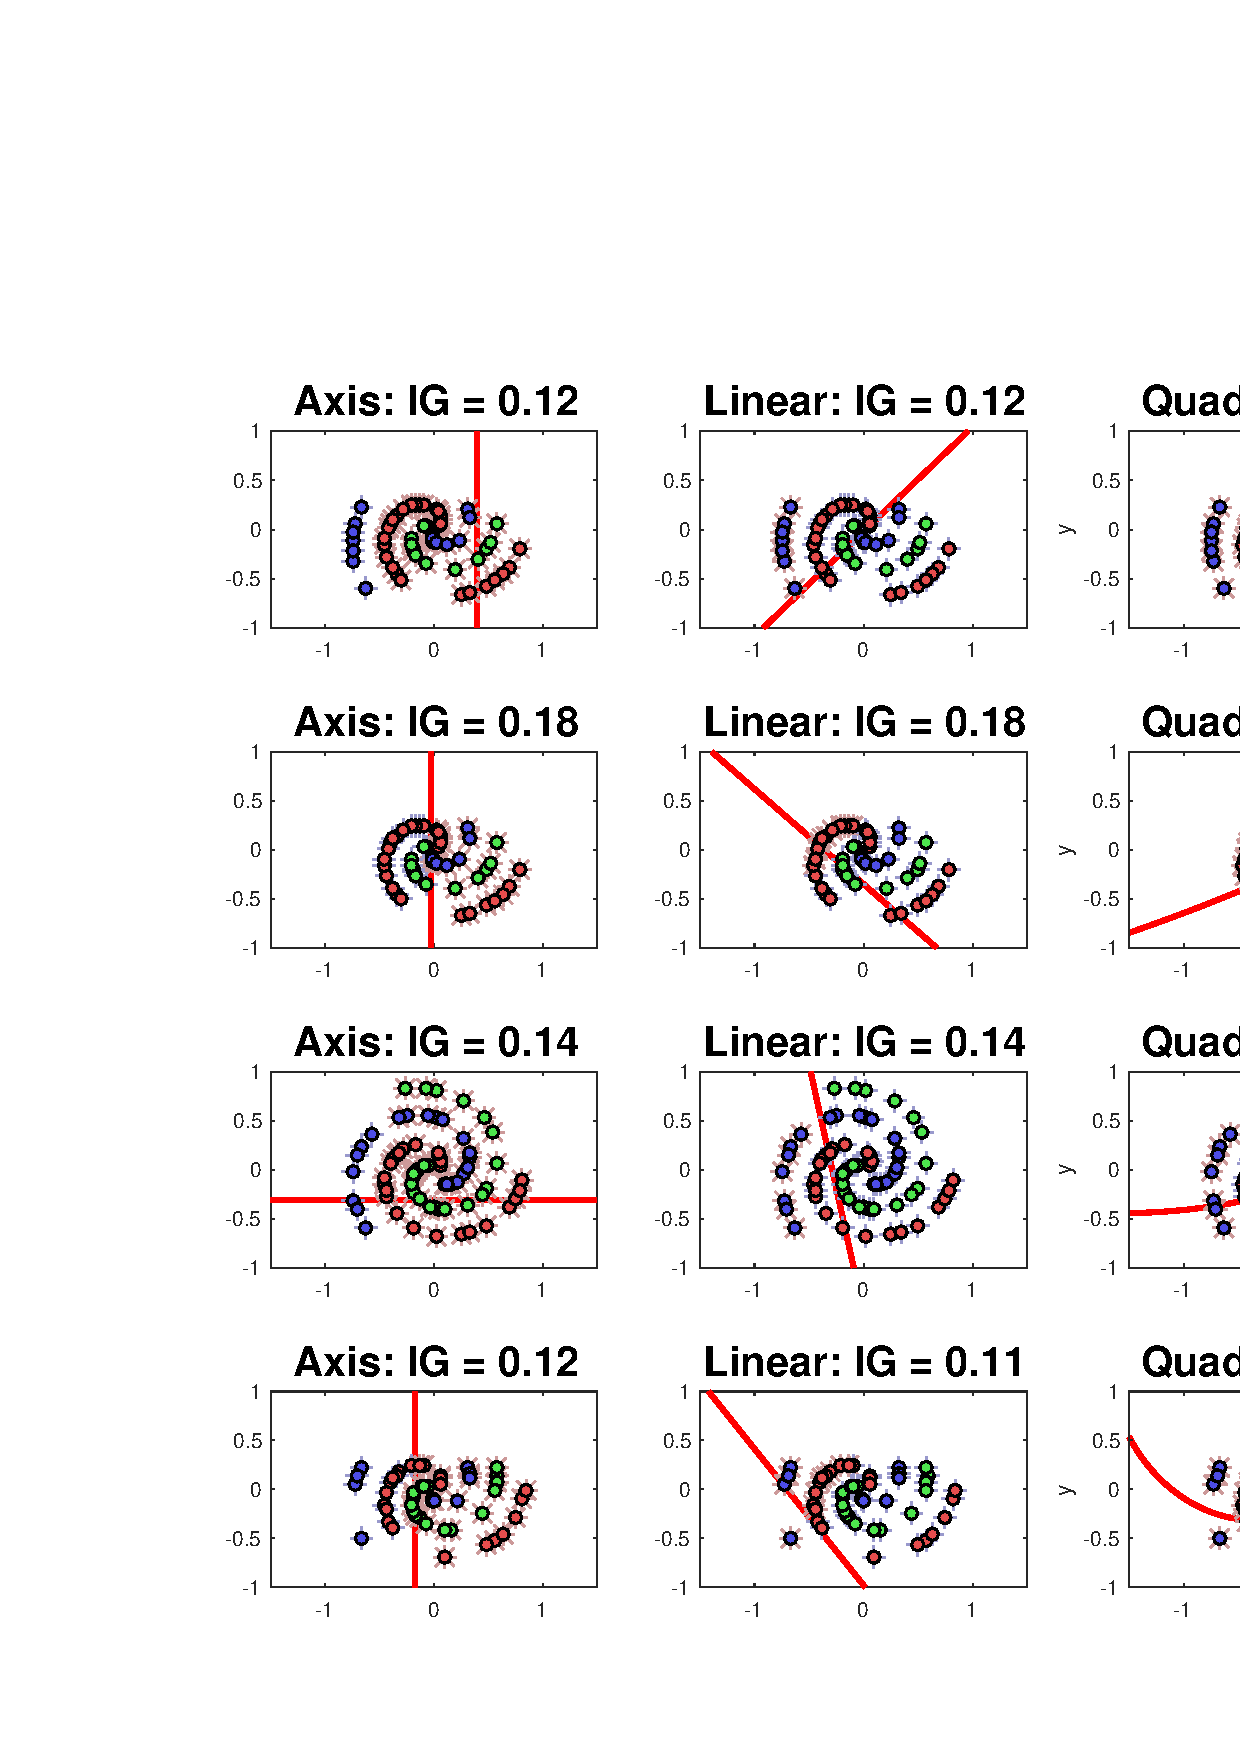
\includegraphics[width=0.60\columnwidth]{split_function_visualitions_5}
    \caption{Overview of spectral subtraction process}
    \label{fig:learners_3}
\end{figure}

Using a stronger learning class such as the quadratic or cubic non-linear functions has it benefits. They can increase the information gain at each node. However, when increasing the strength of the learning class one should also increase the number of split functions tested.

\subsection{Growing Tree}
The leaves visualized in the figure below were generated by growing a tree that utilizes axis-aligned weak-learners. Most leaves contain only one class of data points; the recursive splitting of the data points down the tree has a distilling effect. There are some leaves with 2 or more classes of data. This can be attributed to the difficulty in isolating classes near the origin where the training data is tightly clustered.

\begin{figure}[H]
	\centering
    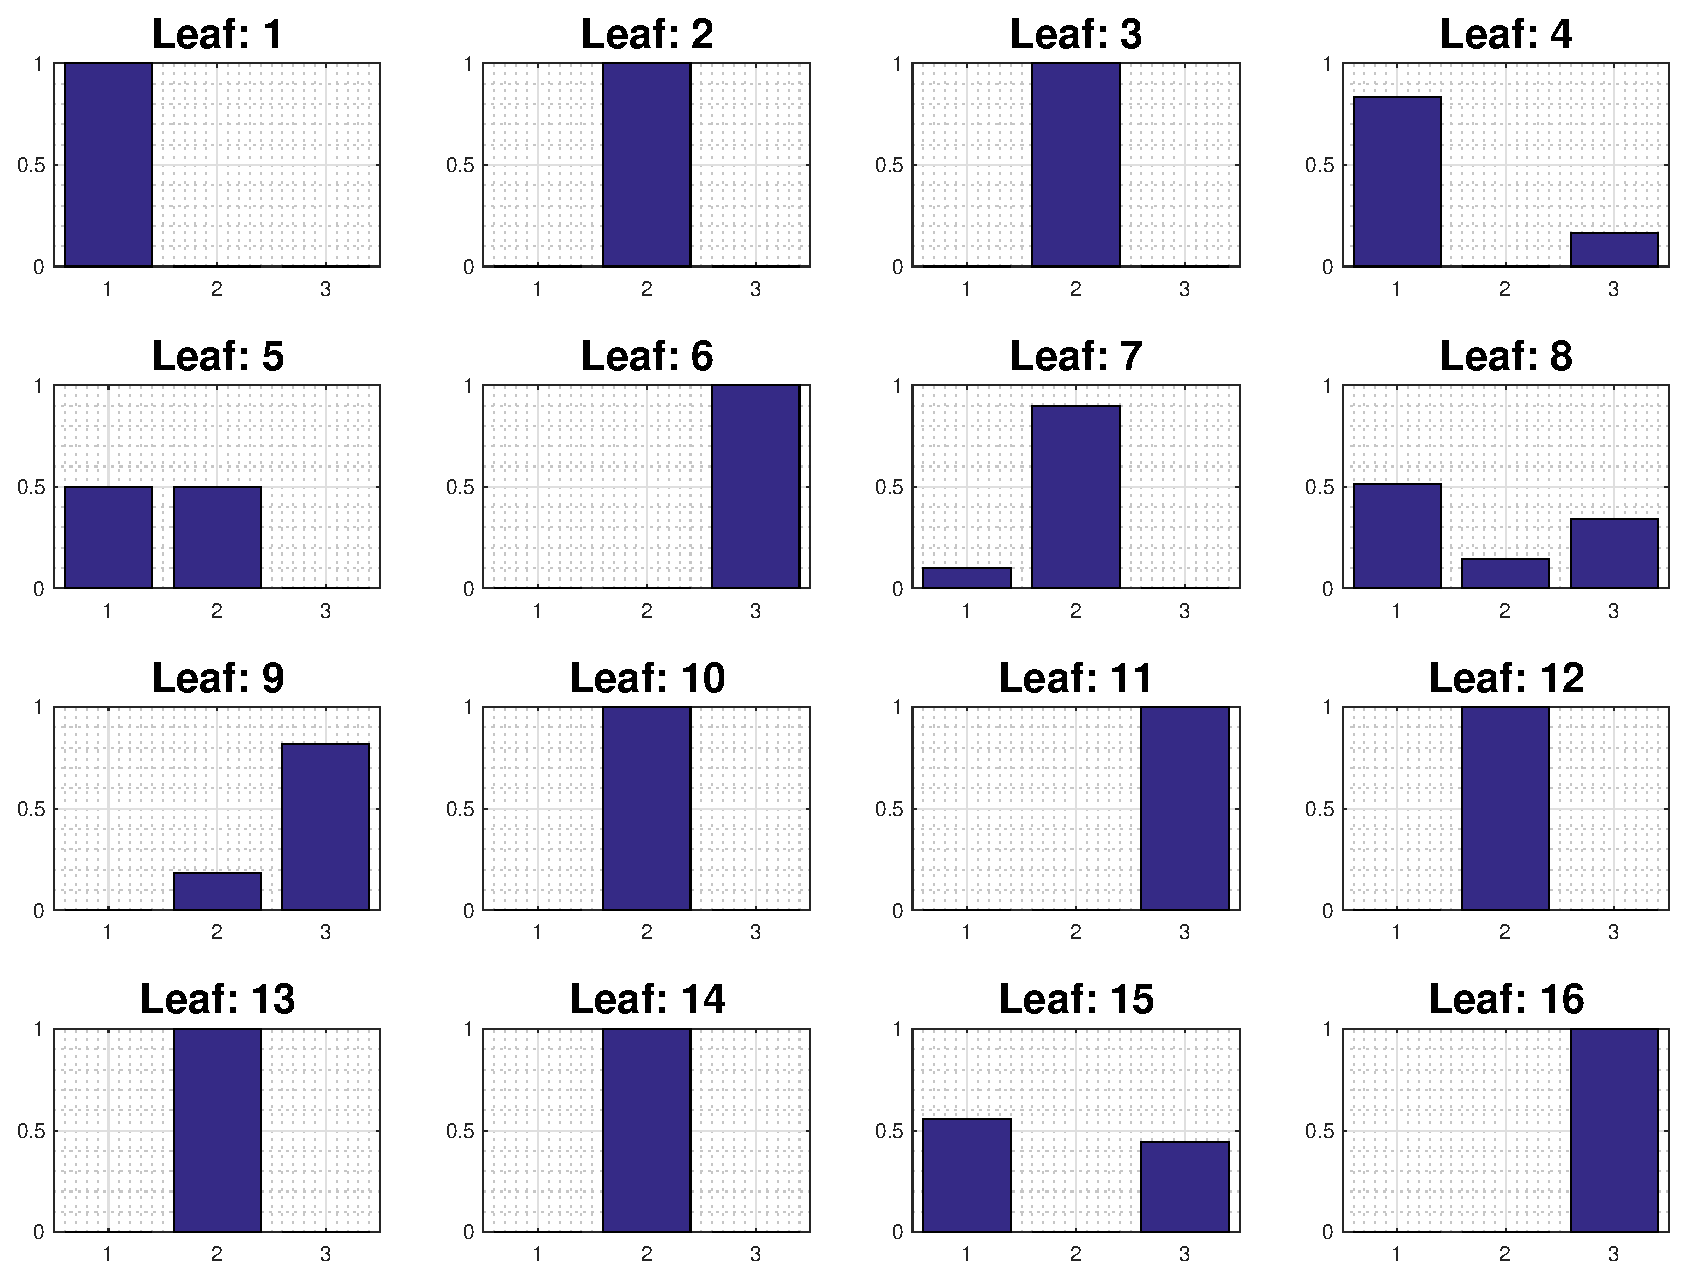
\includegraphics[width=0.60\columnwidth]{leaf_node_distributions_1}
    \caption{Overview of spectral subtraction process}
    \label{fig:leaf_nodes}
\end{figure}

The tree was built using two stopping criteria, used in conjunction. Firstly, a node is considered a leaf if less 5 training points reach it. If only 5 points arrive at a node, they will be concentrated within a small region. Training based on these points will lead to over-fitting. The second stopping criteria is the maximum tree depth. This is simple to implement and gives us direct control on the maximum number of leaves. Using the tree-depth to control the number of leaves will come in handy when growing an Random Forest codebook.

\section{Evaluating Decision Forest}

\begin{figure}[H]
	\centering
    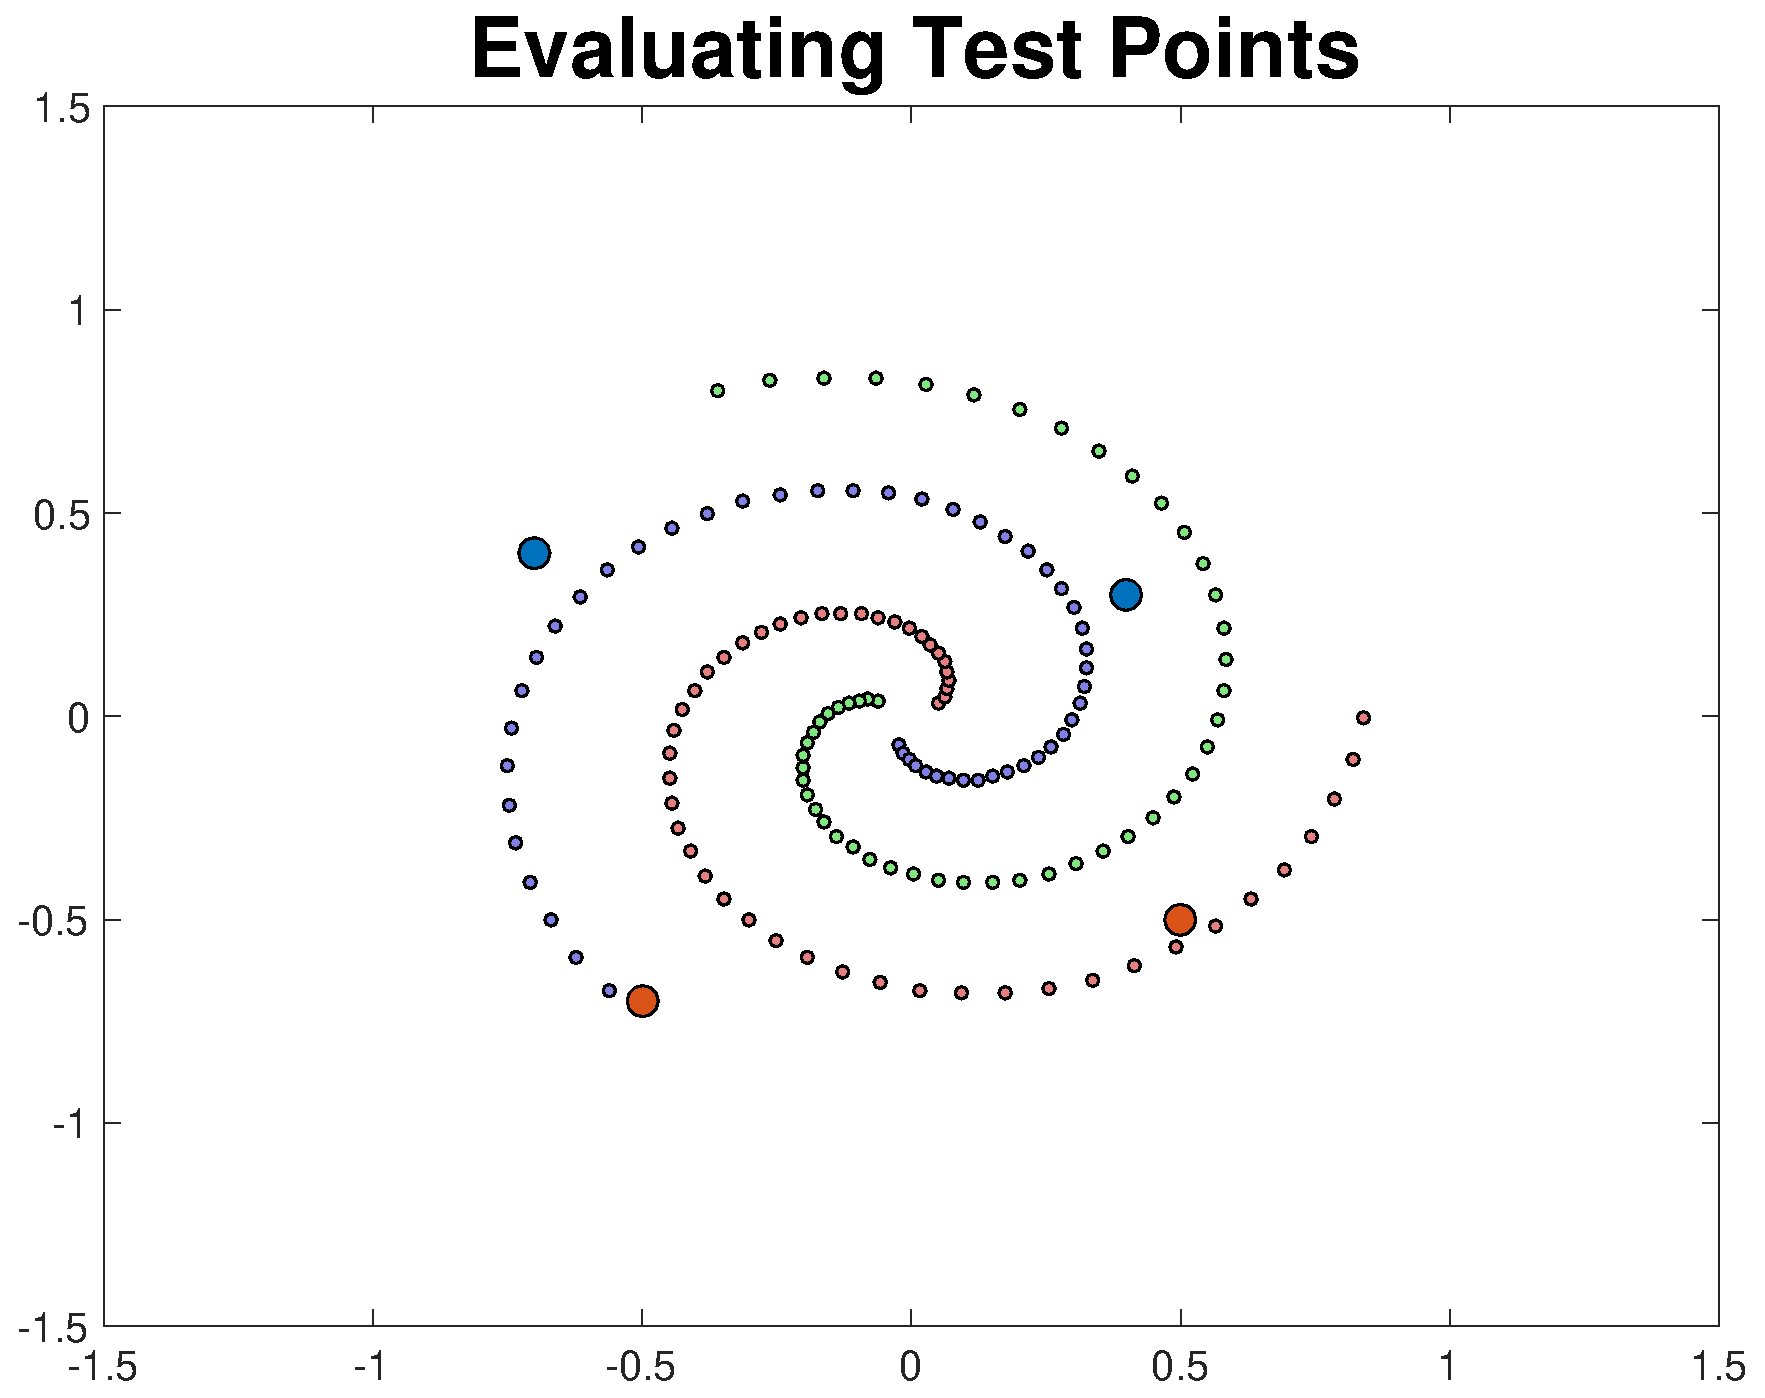
\includegraphics[width=0.49\columnwidth]{test_points_eval}
    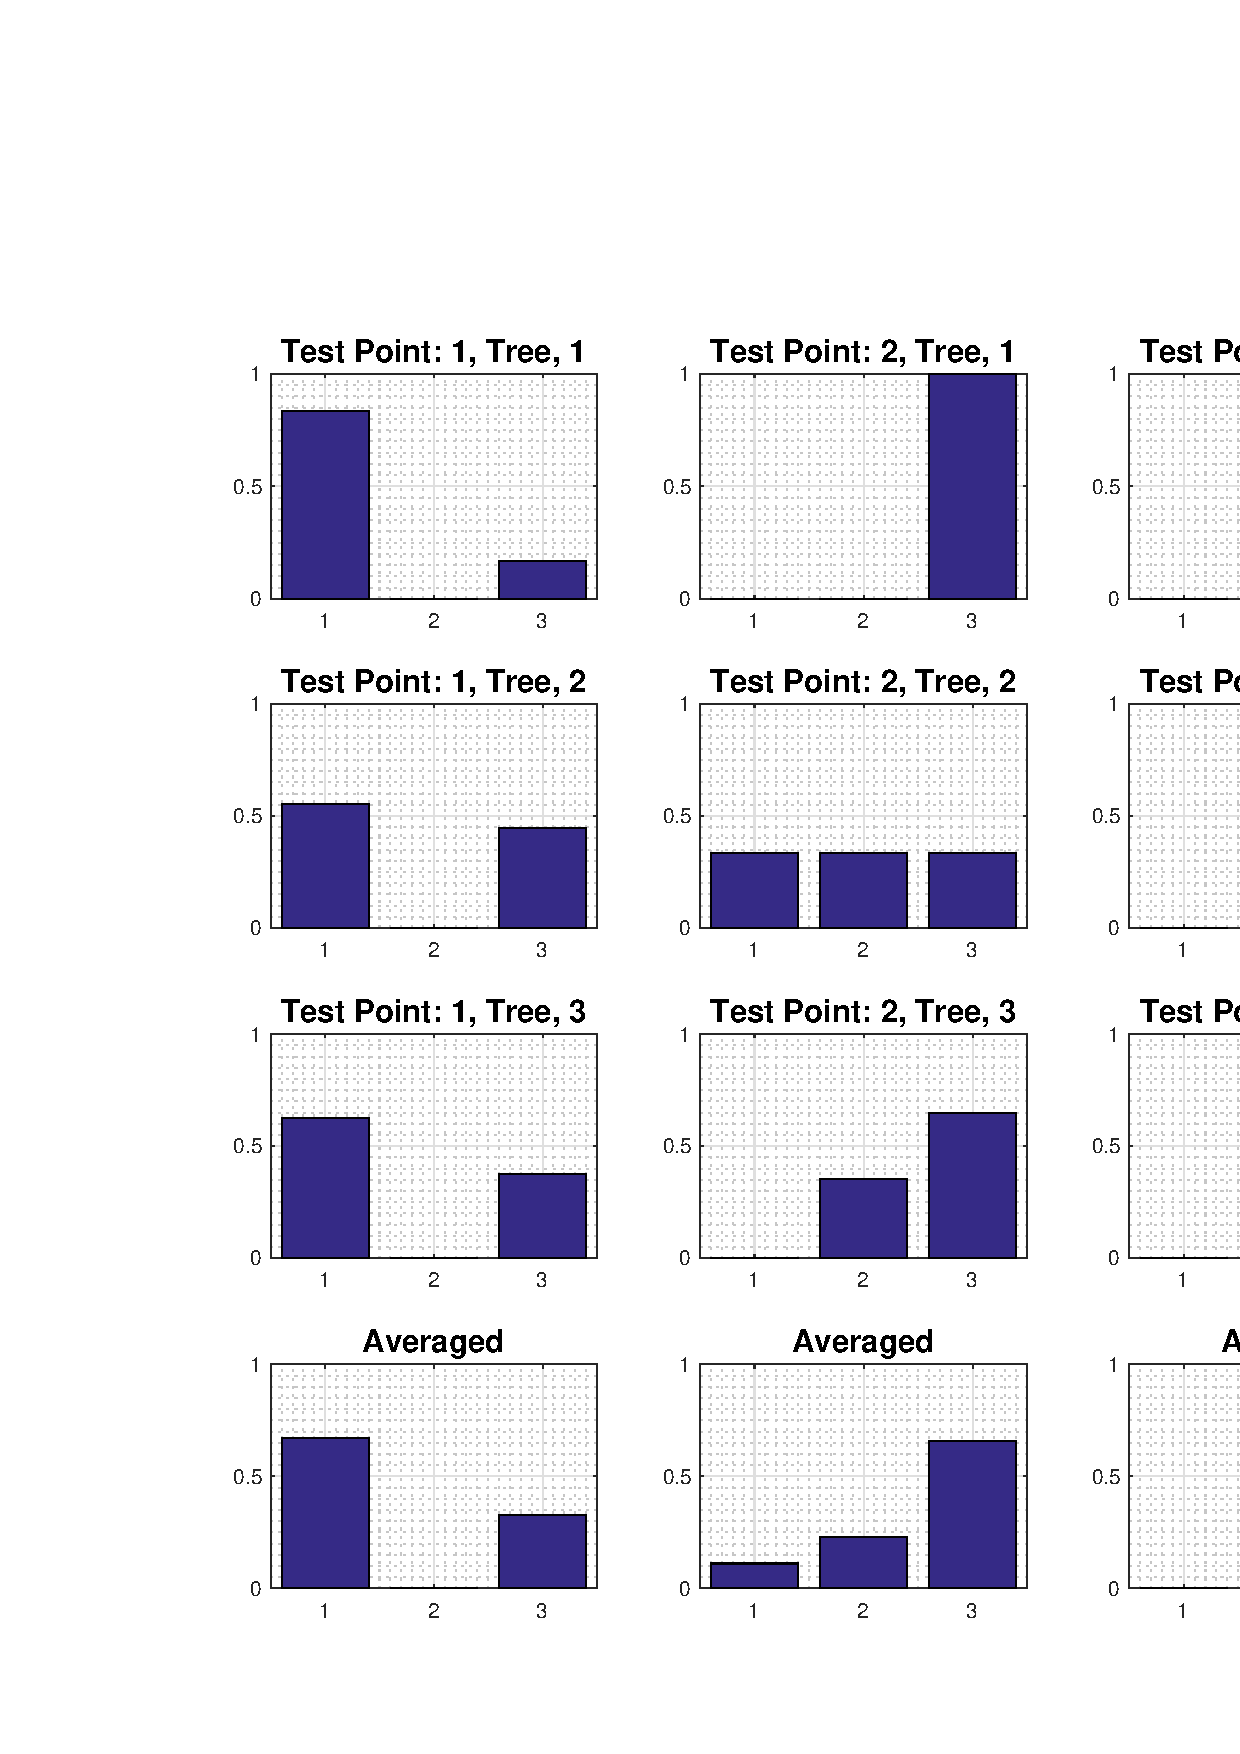
\includegraphics[width=0.49\columnwidth]{test_points_hist}
    \caption{Overview of spectral subtraction process}
    \label{fig:leaf_nodes}
\end{figure}


The 4 test points are evaluated on a forest containing 3 trees; the results obtained are visualized above. The histograms show the probability distribution functions at each leaf for each point. The averaged values have also been plotted. Note that test point 1 (-0.5, -0.7), has been mis-classified; ideally, the point should be blue. The reasons for this misclassification is multi-fold. One of the main factors is that he random forest only has 3 trees and thus the averaging effect of the committee machine is limited.

\subsection{Varying Number of Trees}

To directly combat the misclassification observed above, the first parameter that is varied is the number of trees in the forest. The graph below shows that increasing the number of trees has a considerable effect on the classification accuracy. This is especially true when the absolute number of trees is small. Increasing the number of tress from 100 to 200 has negligible effect. Notice the straight axis-aligned class boundaries obtained in the region of the grid for which extrapolation is required. Training data is contained within the unit square whereas the region for which the classifier is tested extends beyond the unit square. The classifier is expected to extrapolate the class boundaries. Since the axis-aligned weak-learner is used, straight axis-aligned lines are observed in the extrapolated region. 

\begin{figure}[H]
	\centering
    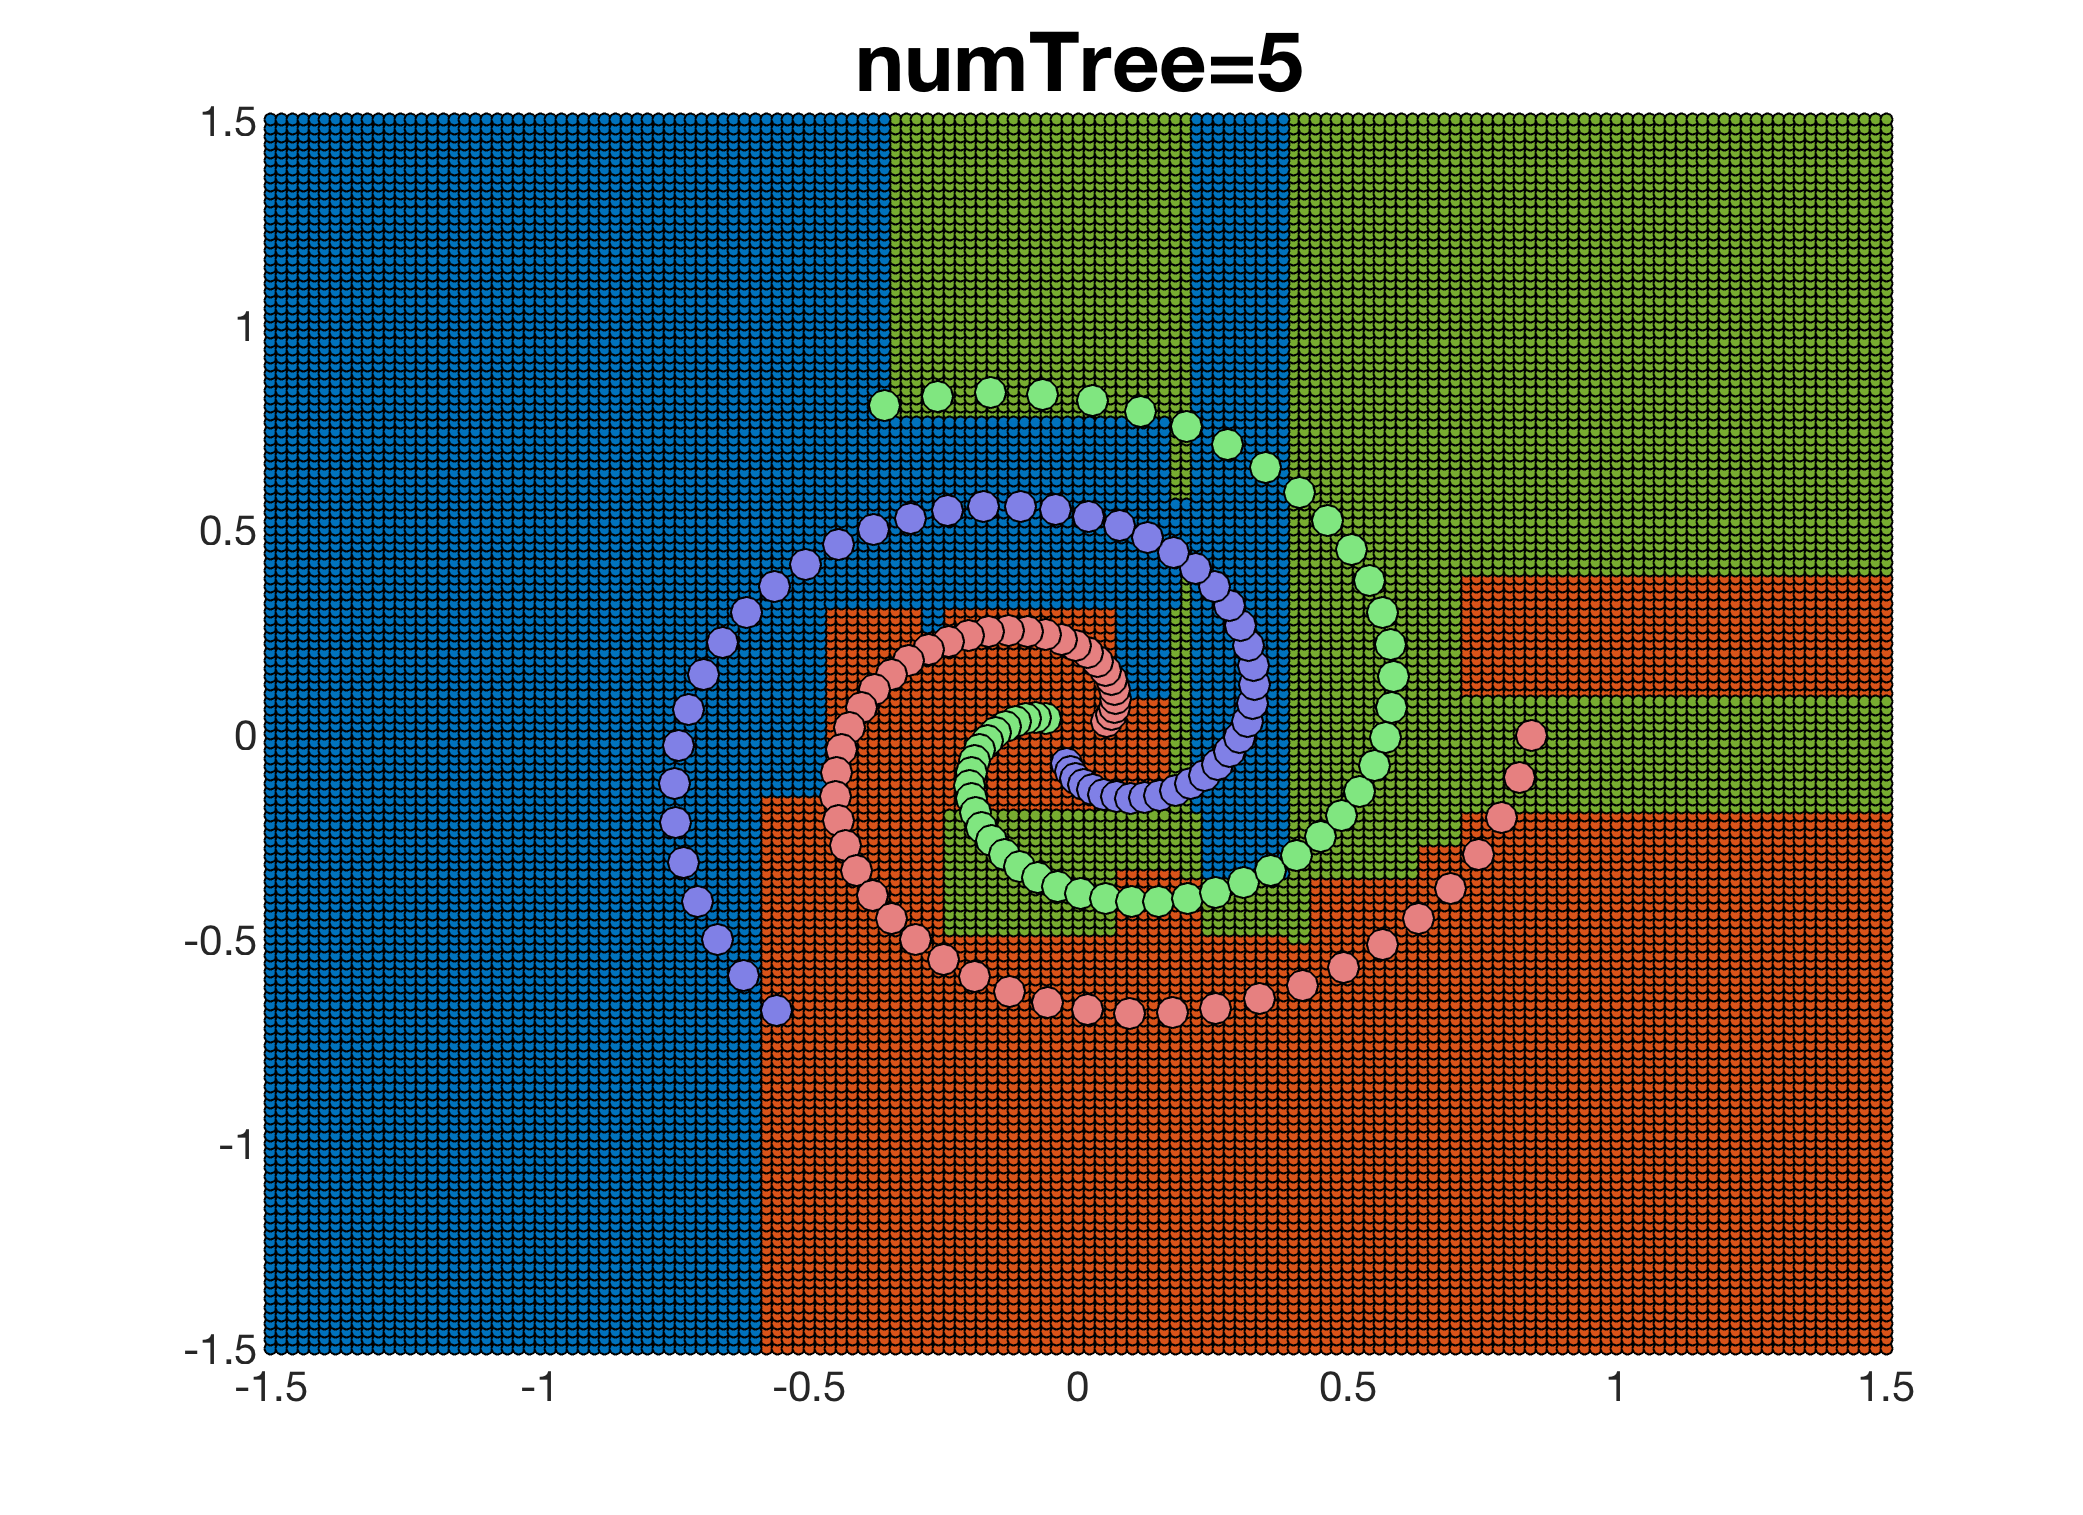
\includegraphics[width=0.40\columnwidth]{ax_5_trees}
	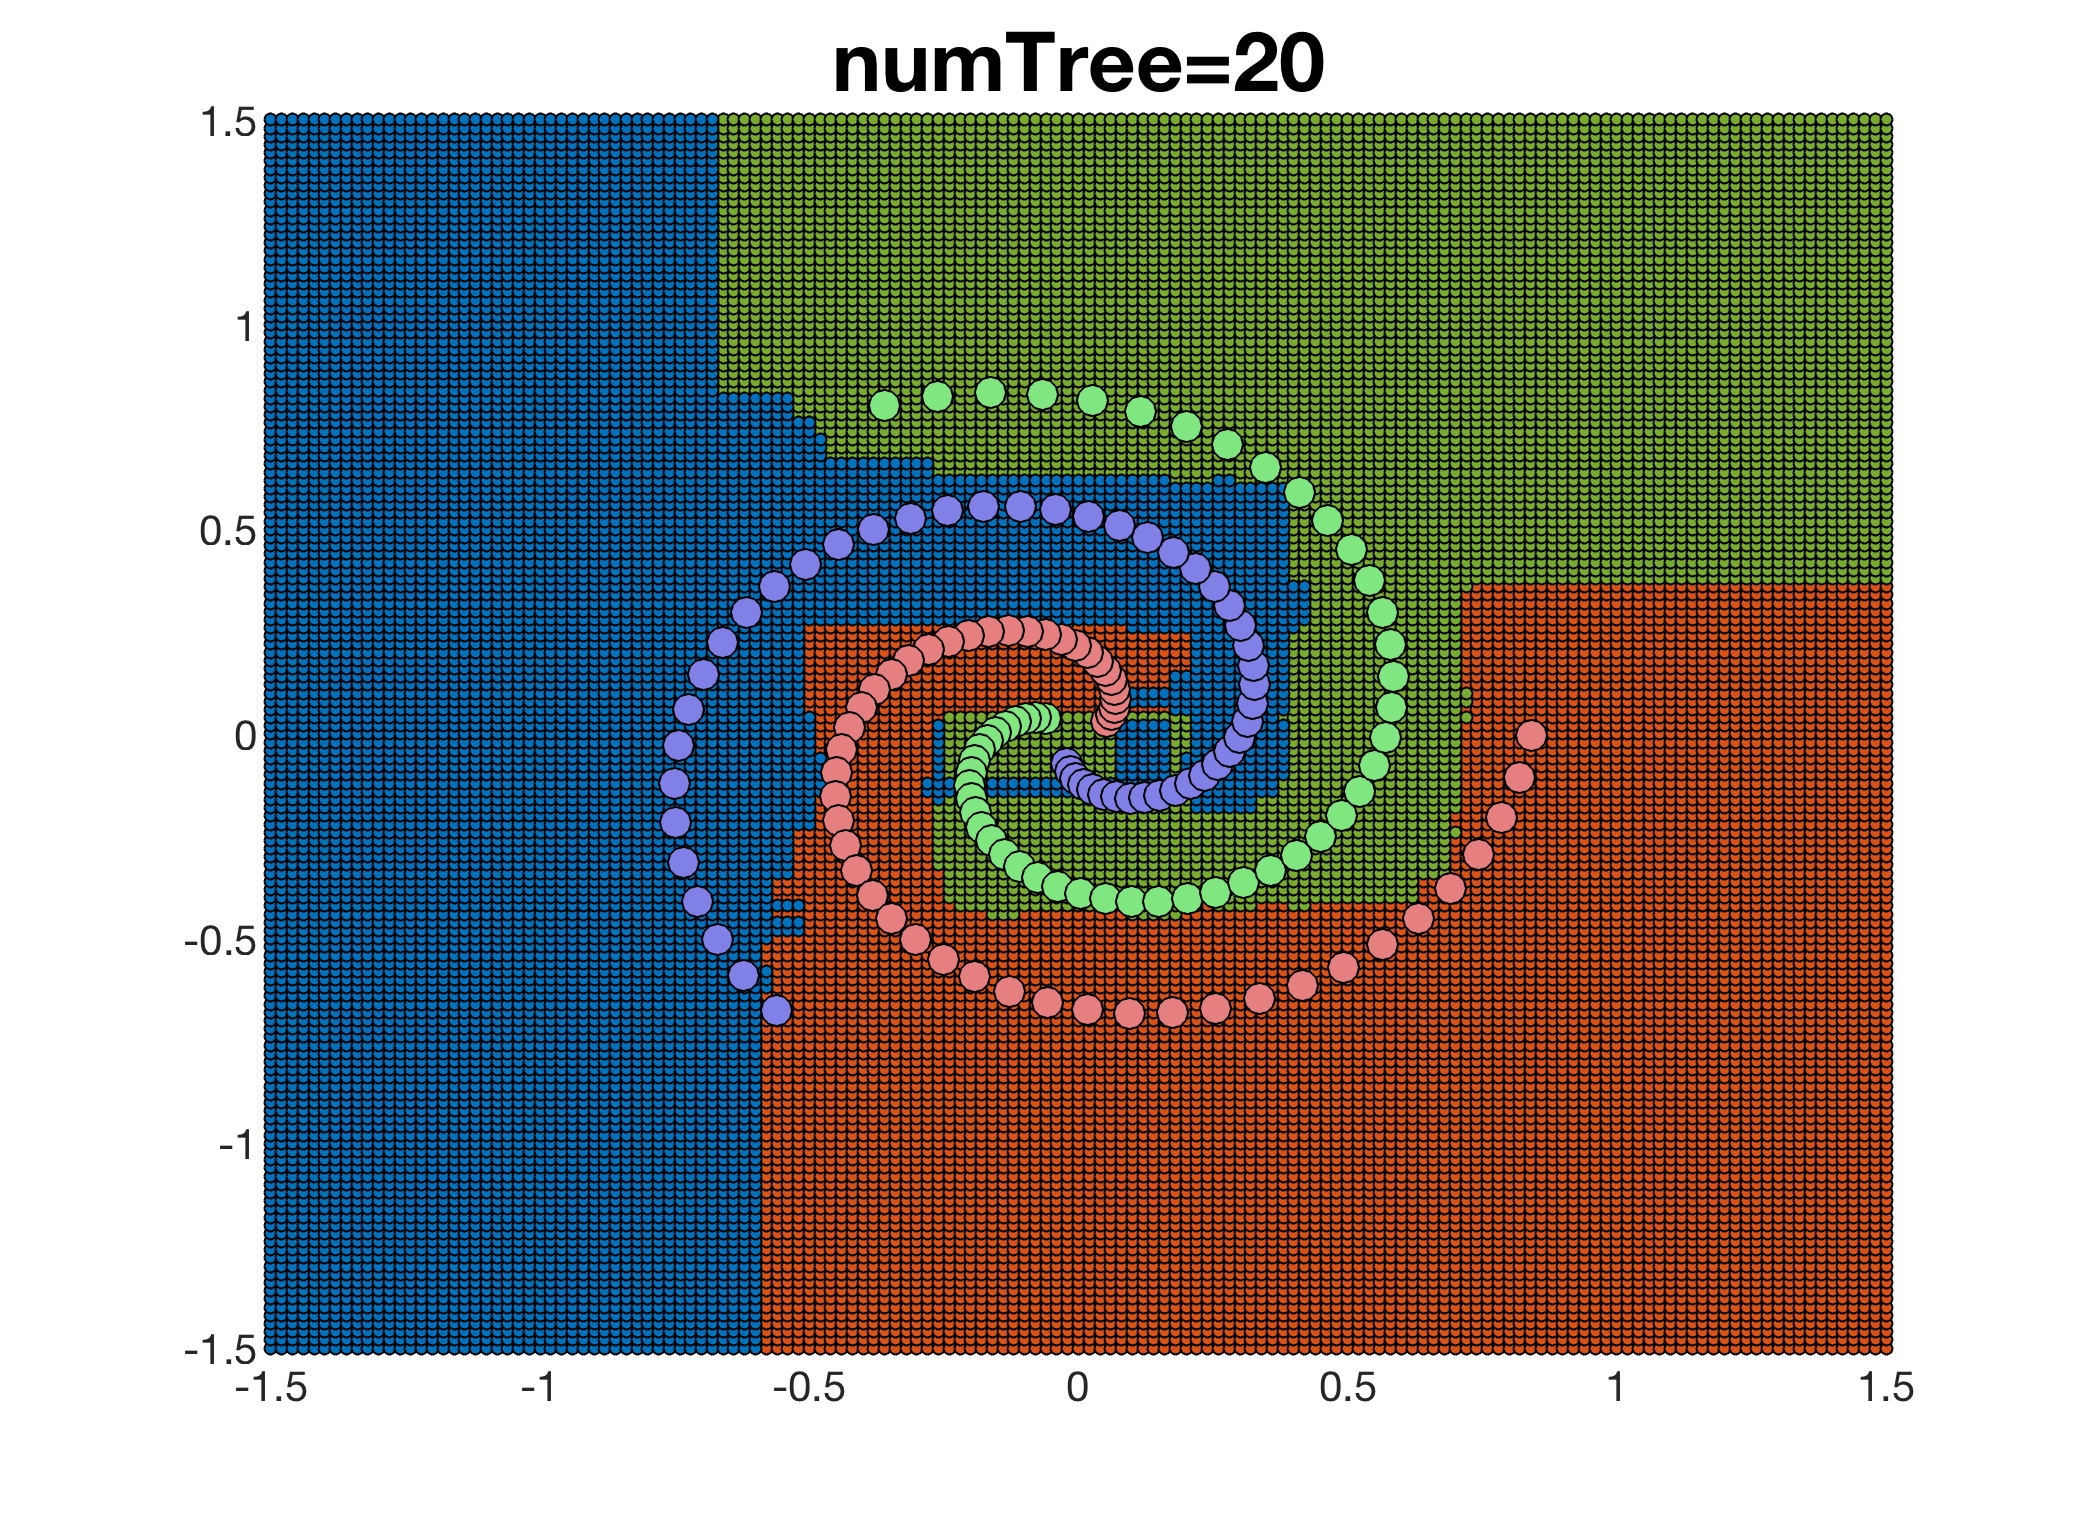
\includegraphics[width=0.40\columnwidth]{ax_20_trees}
    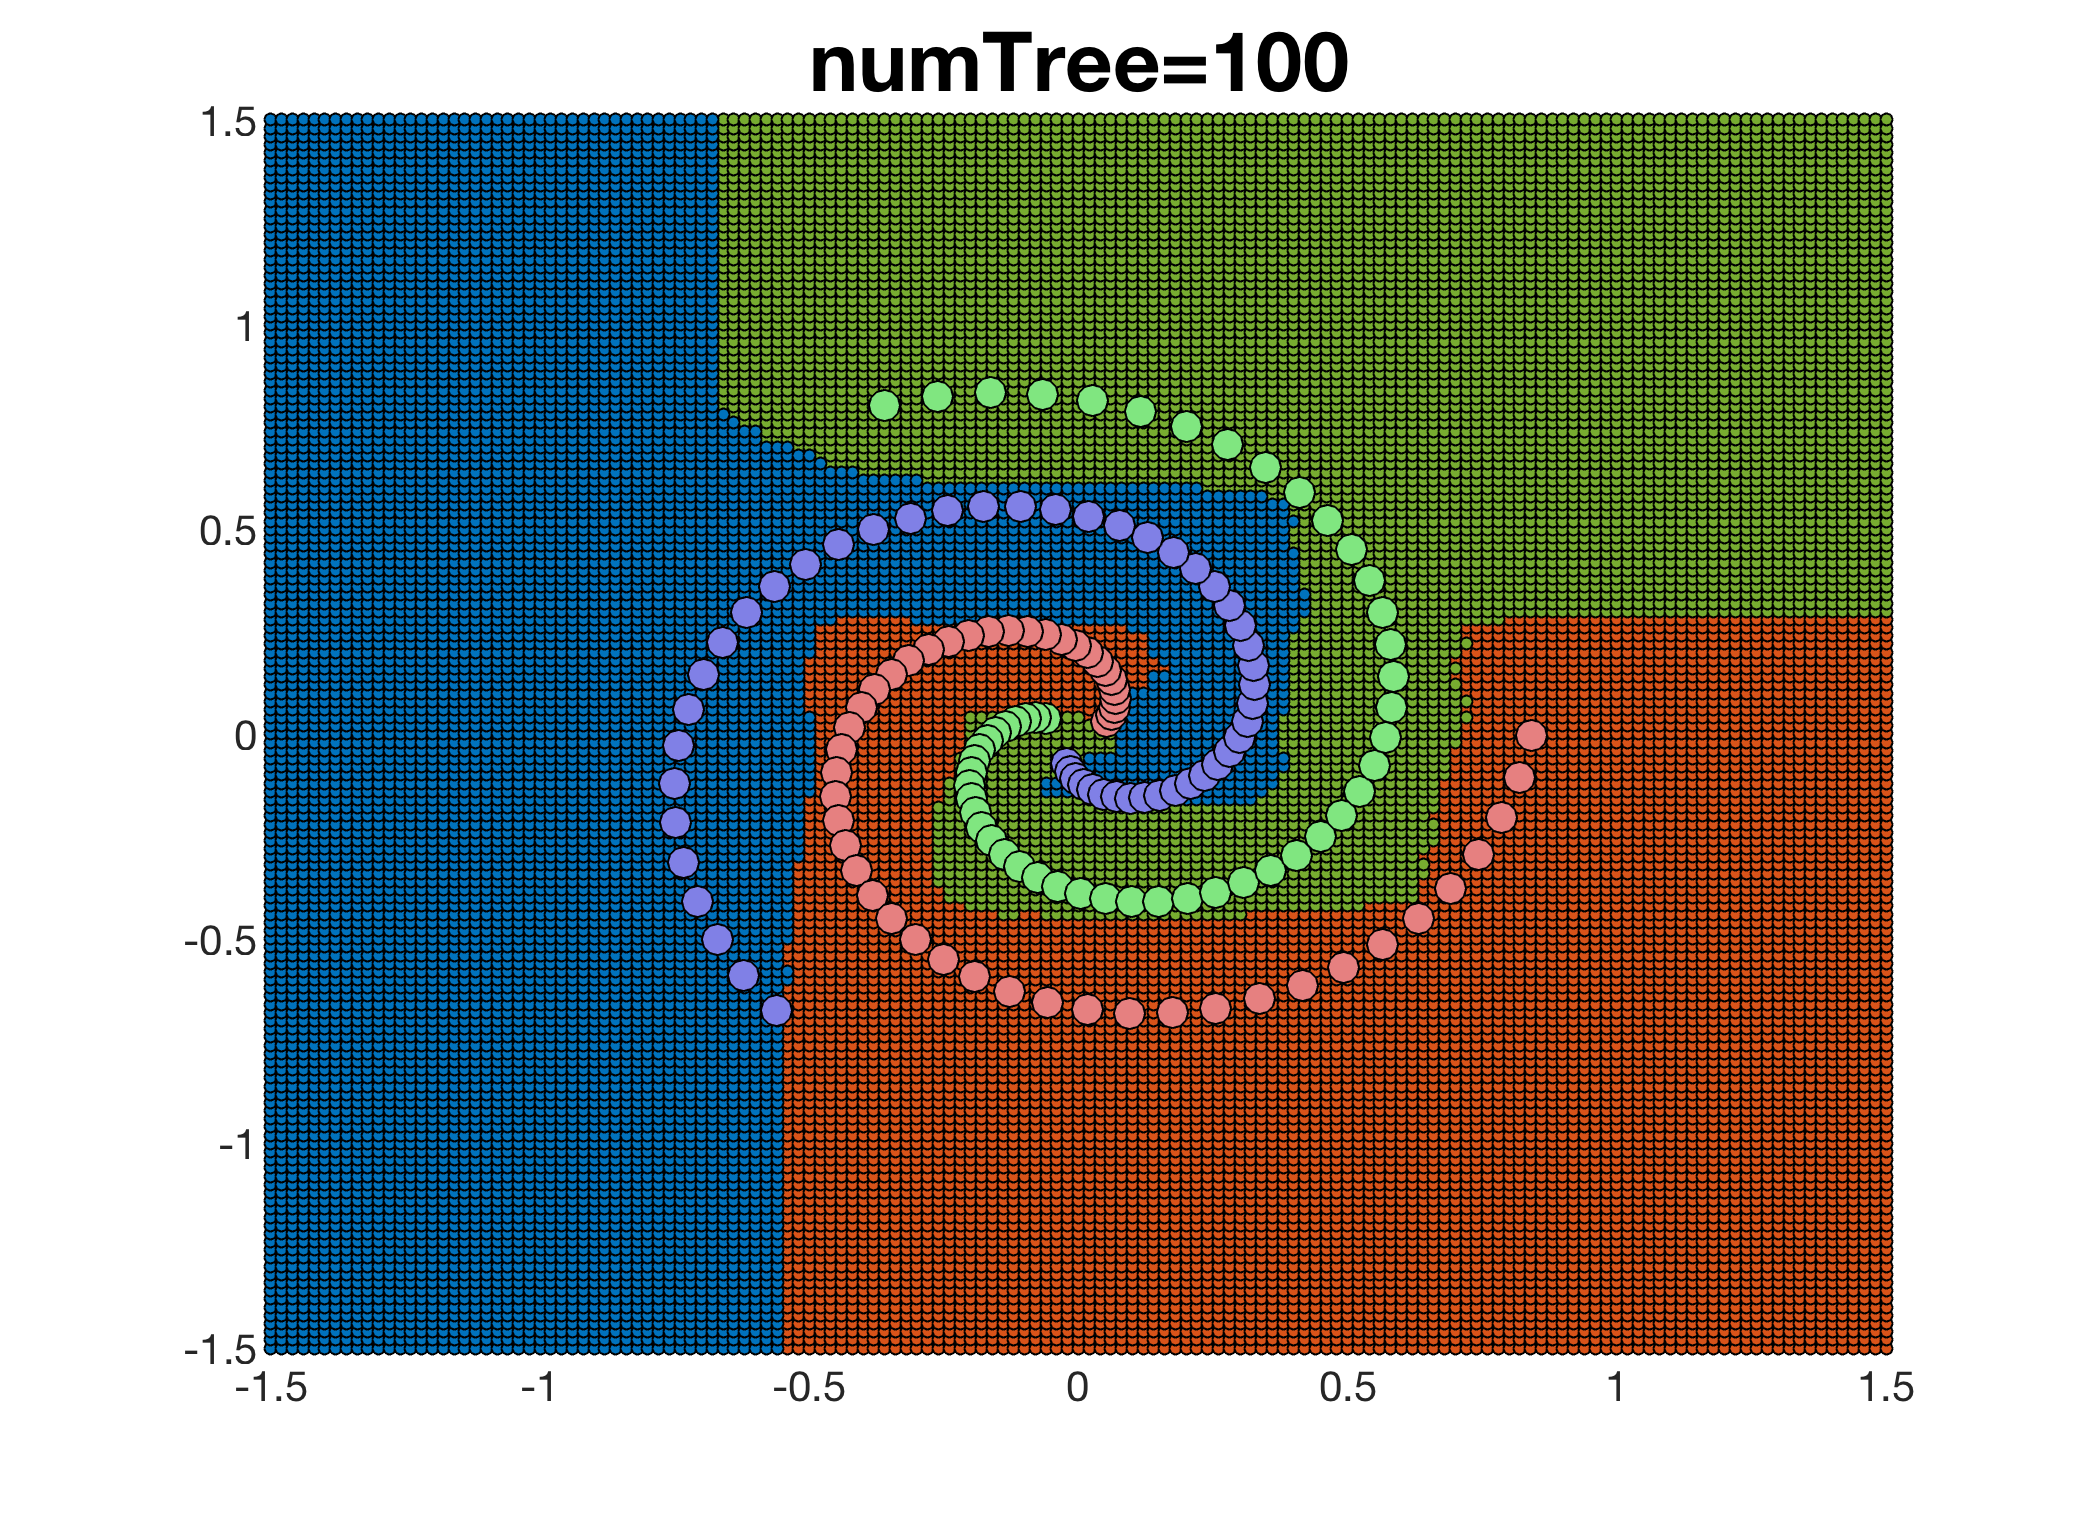
\includegraphics[width=0.40\columnwidth]{ax_100_trees}
    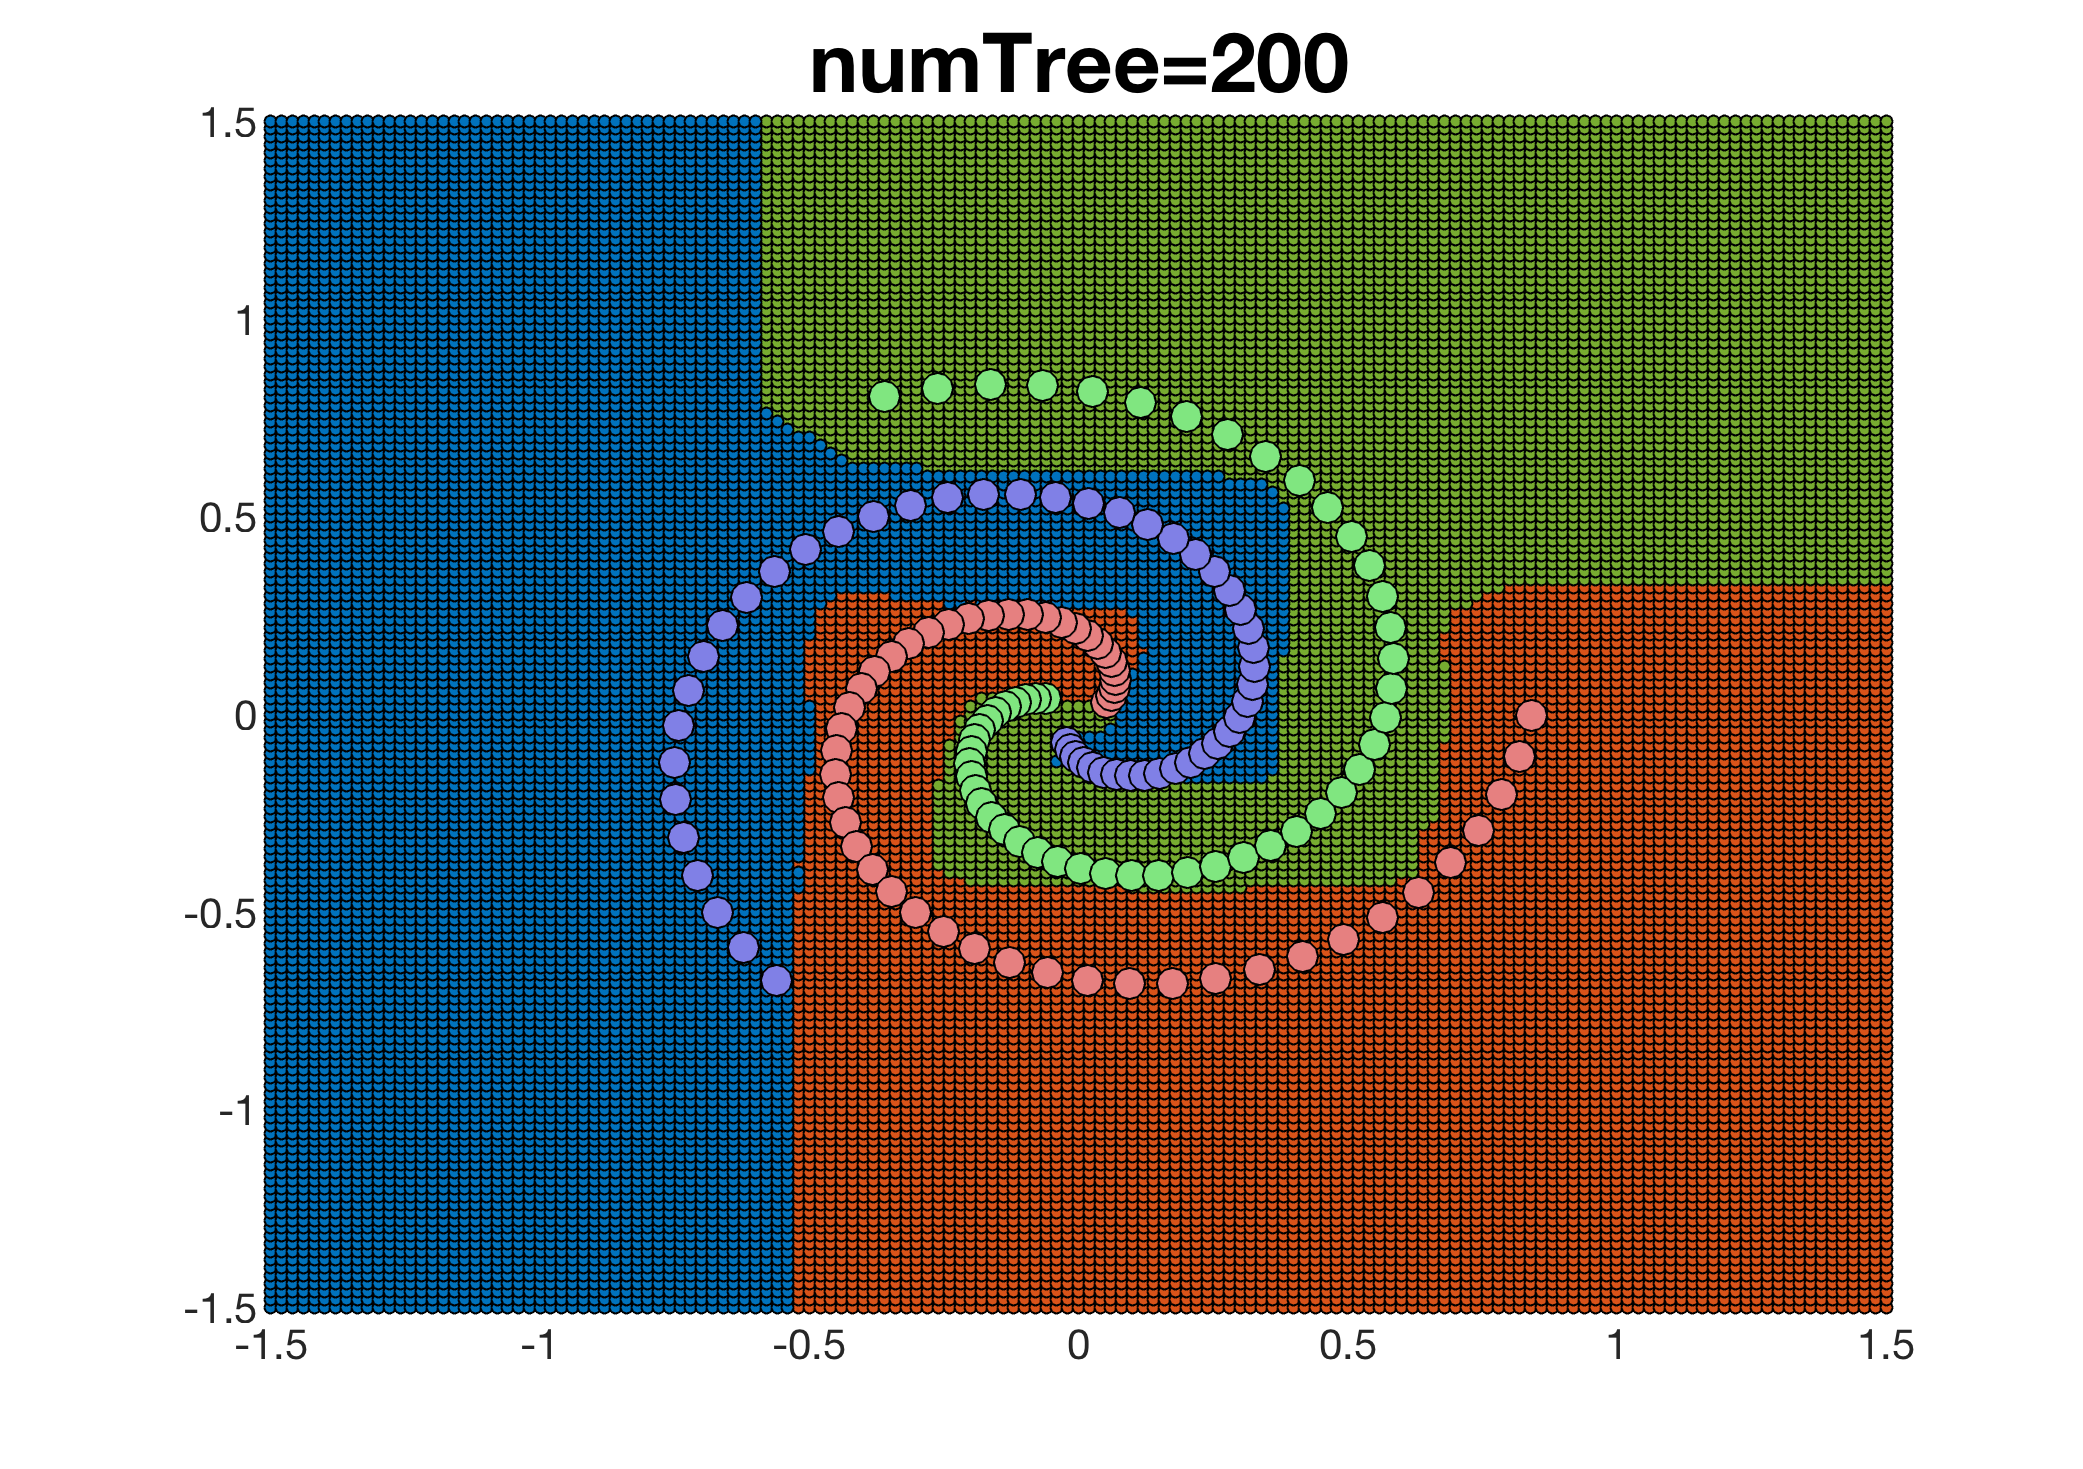
\includegraphics[width=0.40\columnwidth]{ax_200_trees}
    \caption{Overview of spectral subtraction process}
\end{figure}

Increasing the number of trees is not without a cost. The random forest algorithm scales linearly with the number of trees in the forest. The algorithm has the added benefit that it can be parallelised. Each tree can be grown and tested in parallel.

\subsection{Varying Number of Split Functions}

Next, we vary the number of split functions while size of the forest is limited to $10$. By increasing the number of split functions that we try at each node, we are decreasing the inherent randomness within each tree. If all trees are assumed to be completely uncorrelated, then $E_{com}=\nicefrac{E_{av}}{T}$; where $E_{com}$ is the error incurred by the random forest and $E_{av}$ is the average error of each tree. If the trees are correlated, then $E_{com}\leq\nicefrac{E_{av}}{T}$. Even with correlated trees, it is possible that the committee machine produces good results if $E_{av}$ is low. An optimal balance point has to be found; in order to achieve a low $E_{av}$ some correlation between trees is tolerated.

\begin{figure}[H]
	\centering
    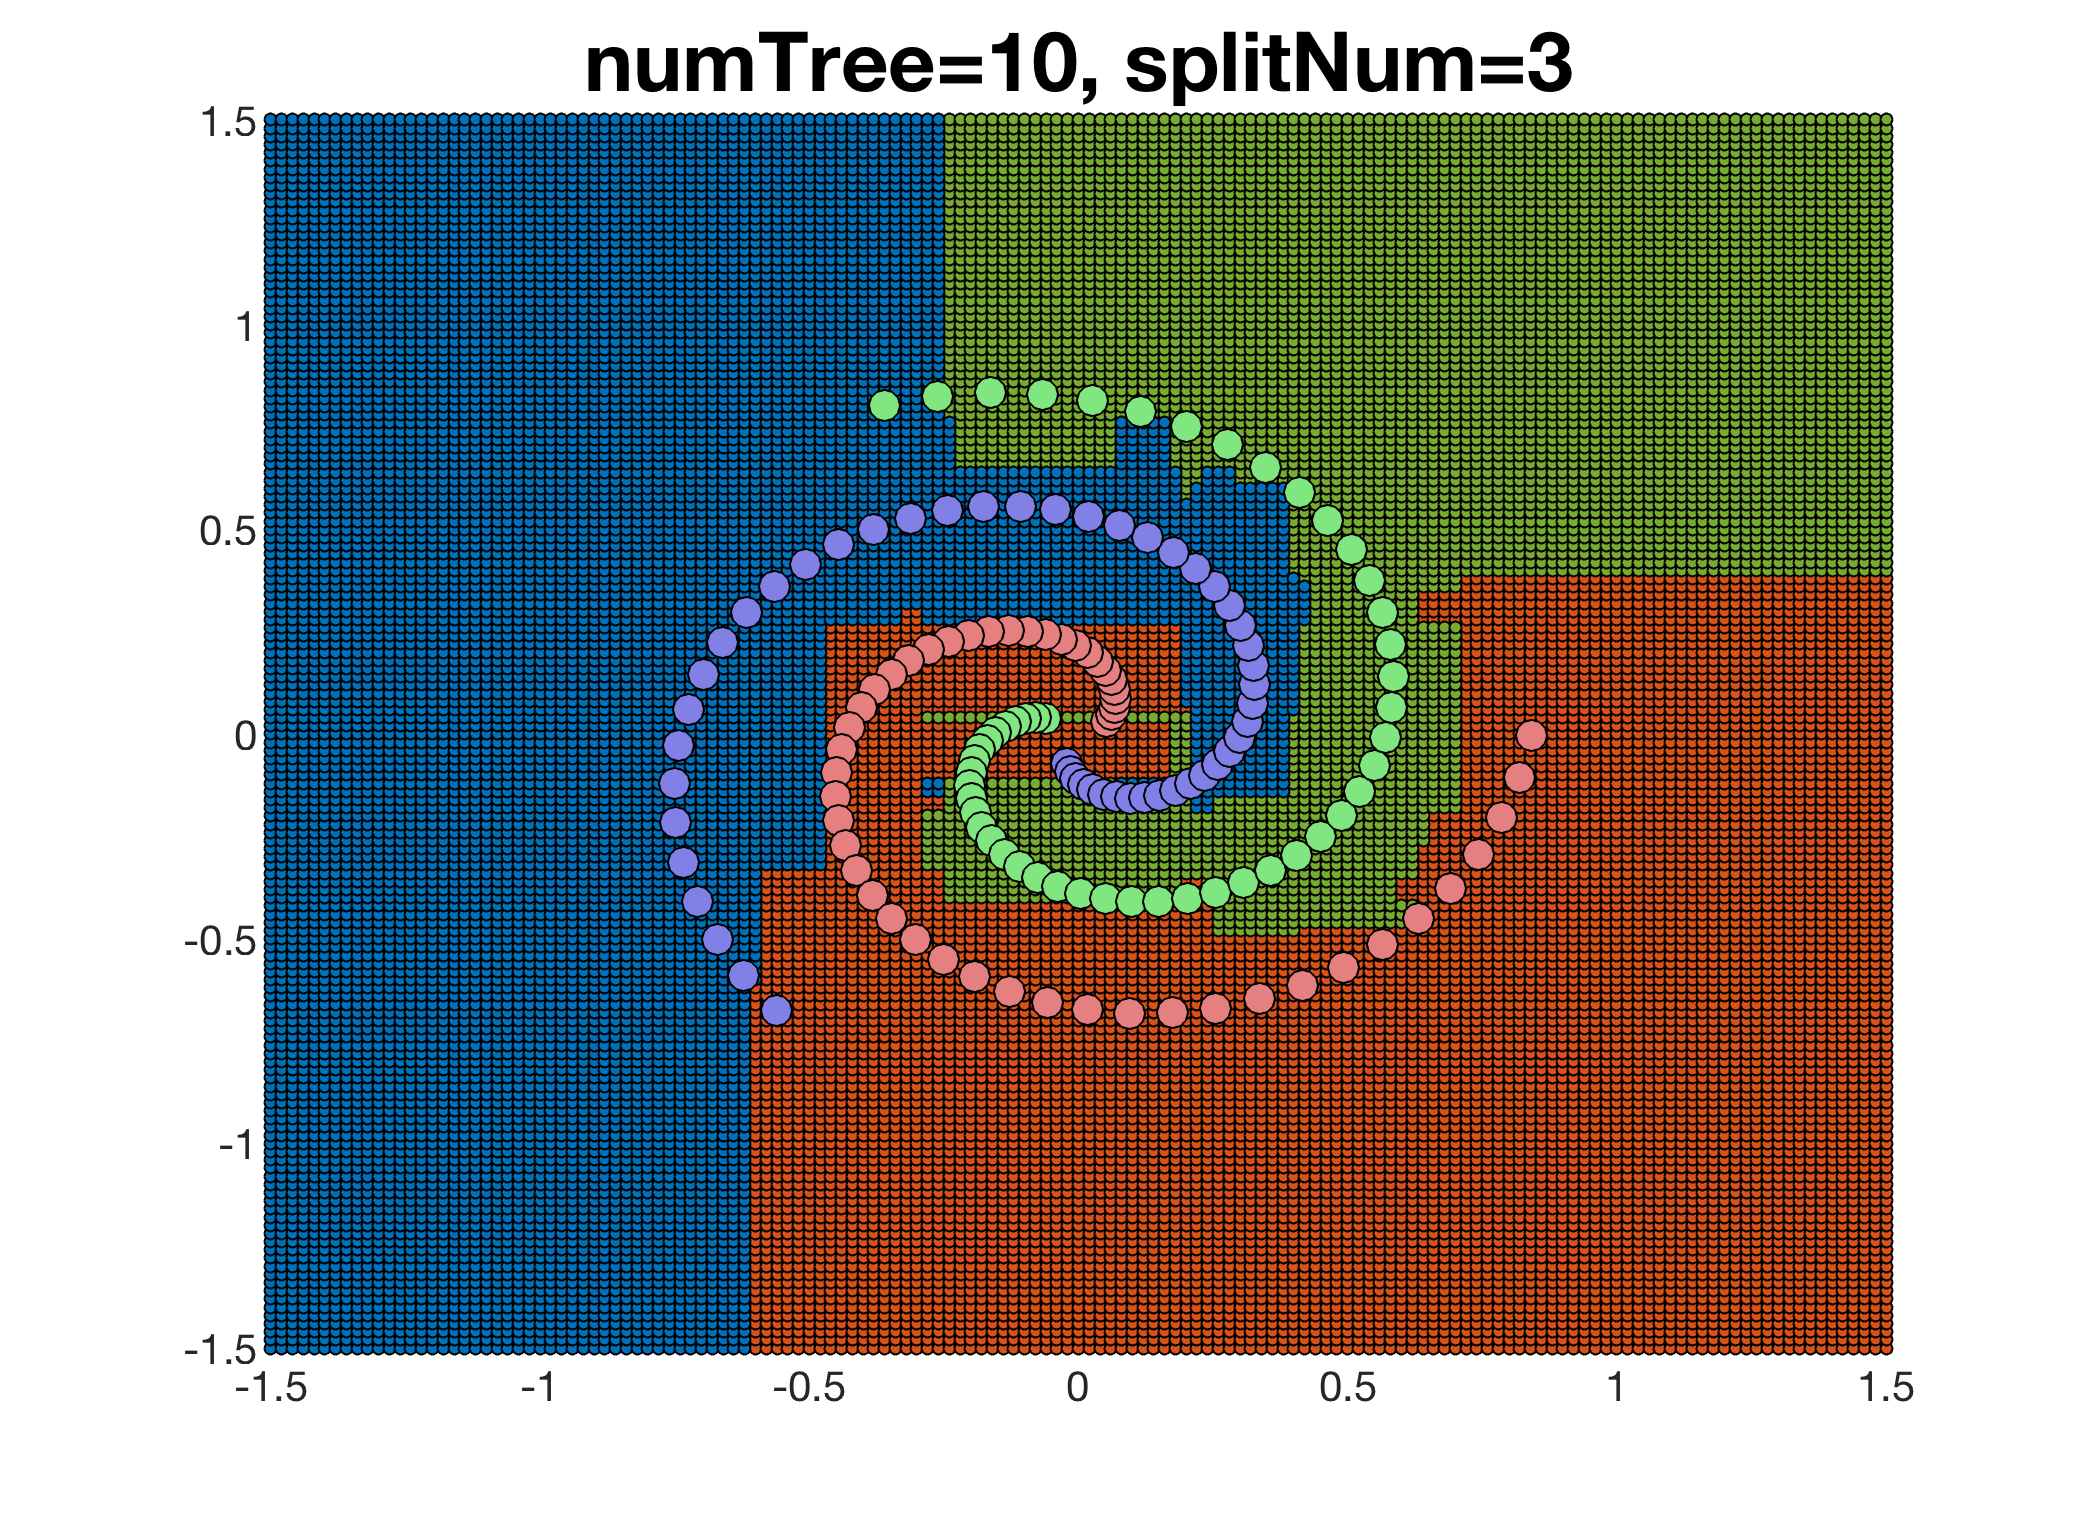
\includegraphics[width=0.40\columnwidth]{splitNum_3}
	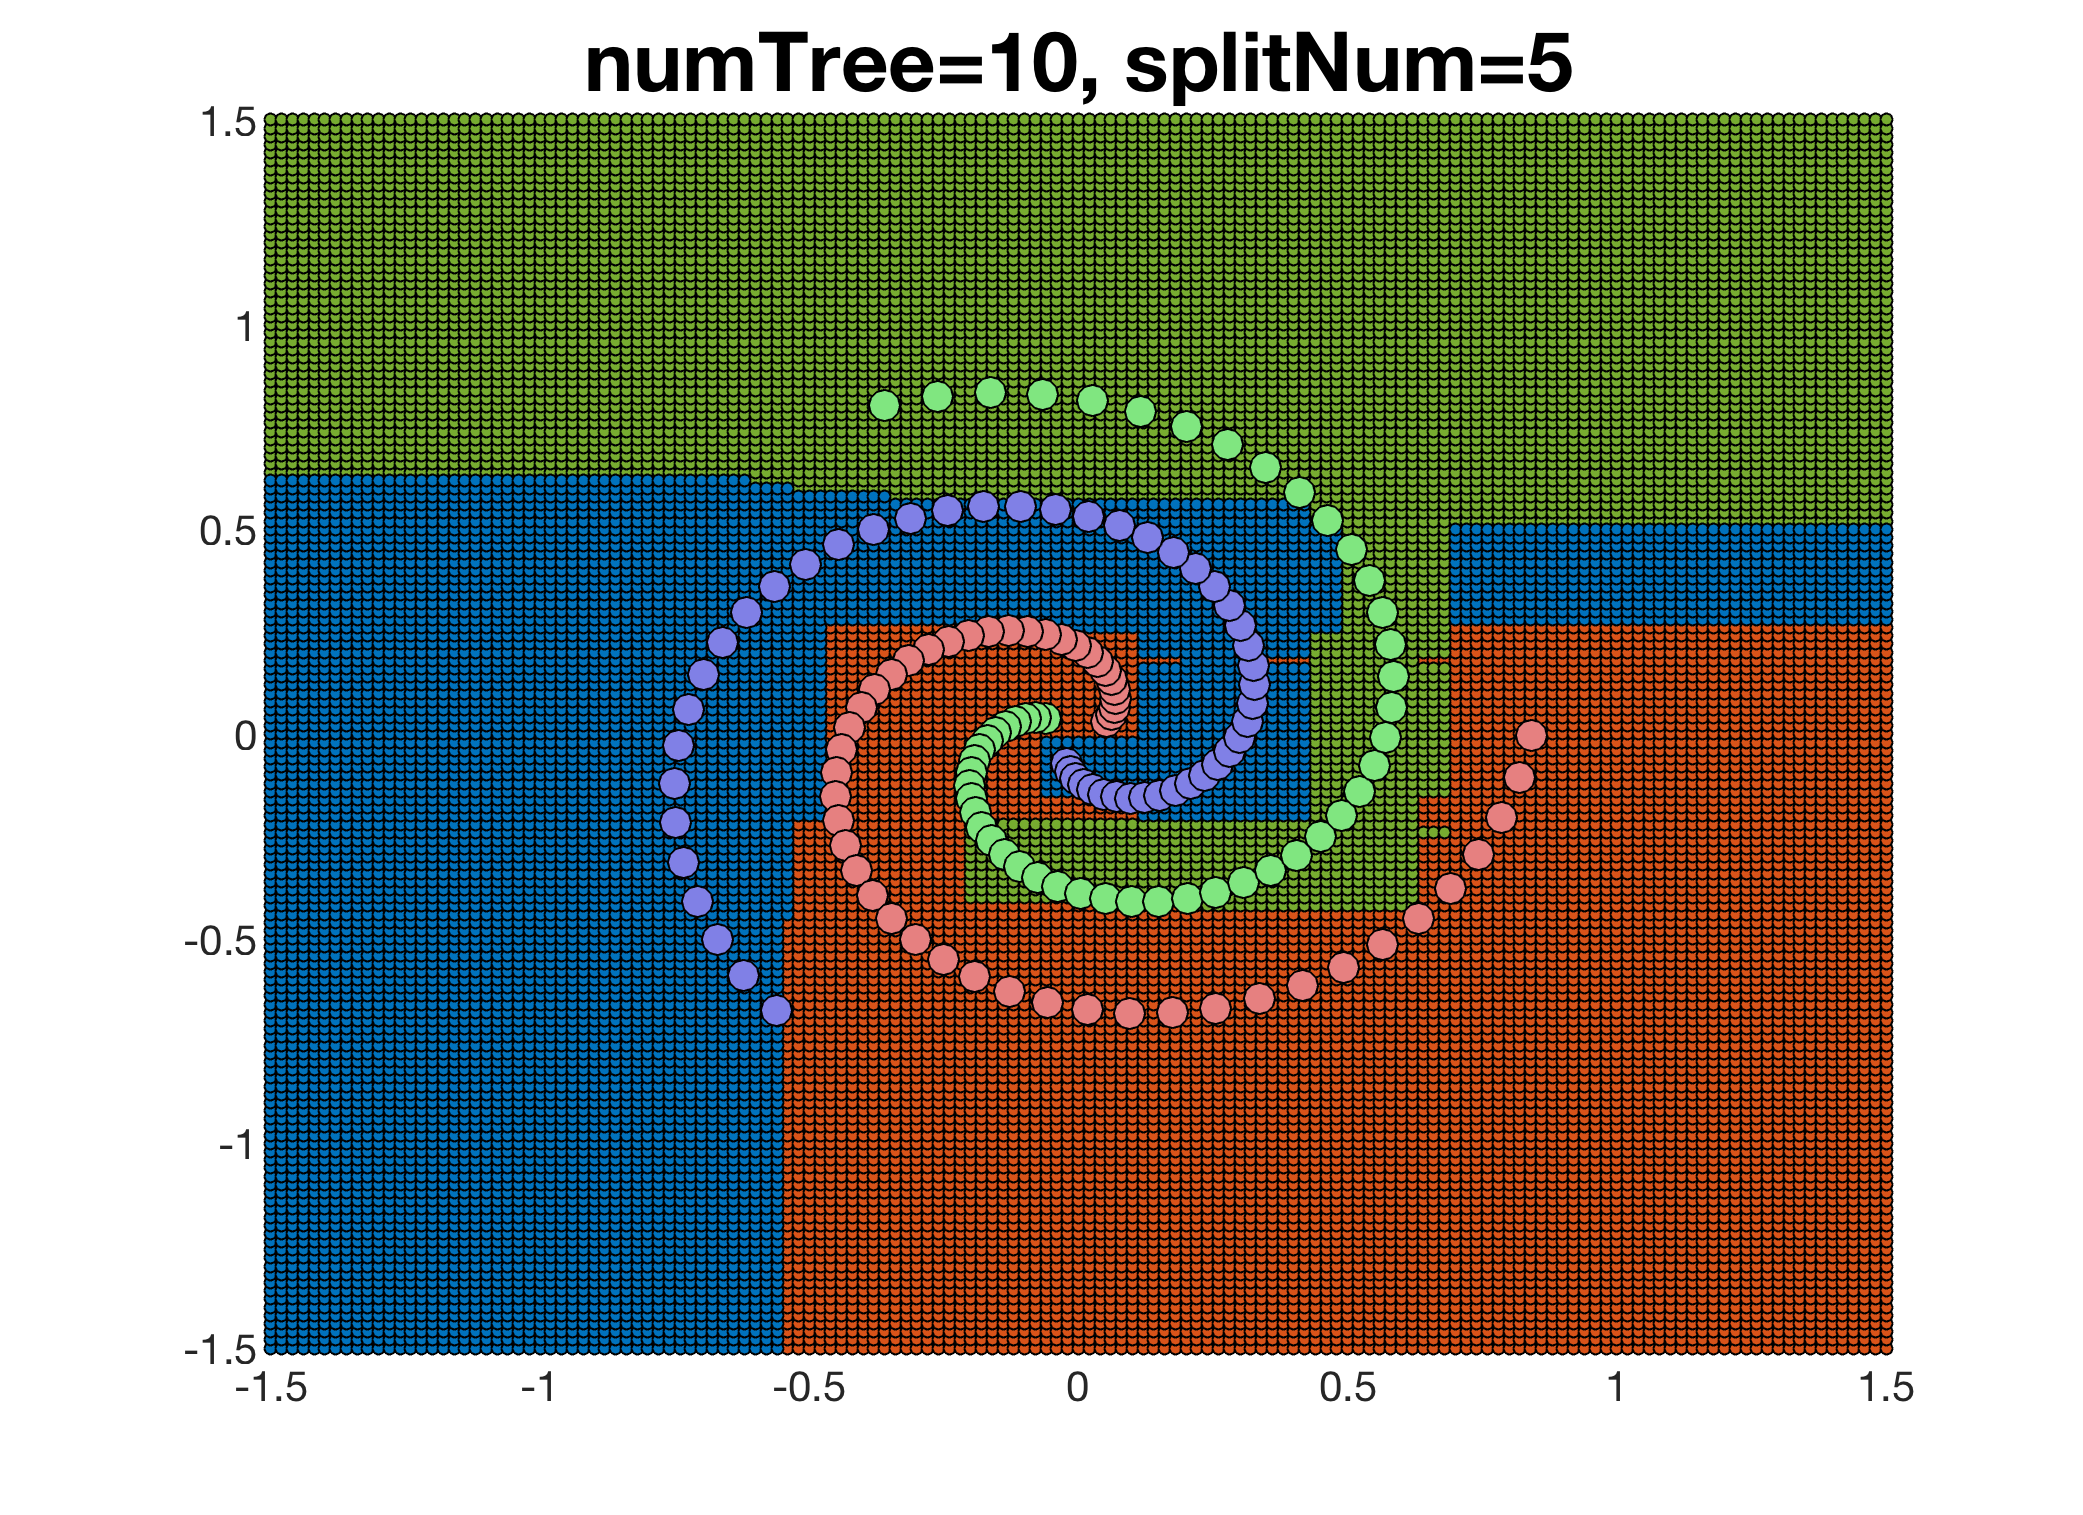
\includegraphics[width=0.40\columnwidth]{splitNum_5}
    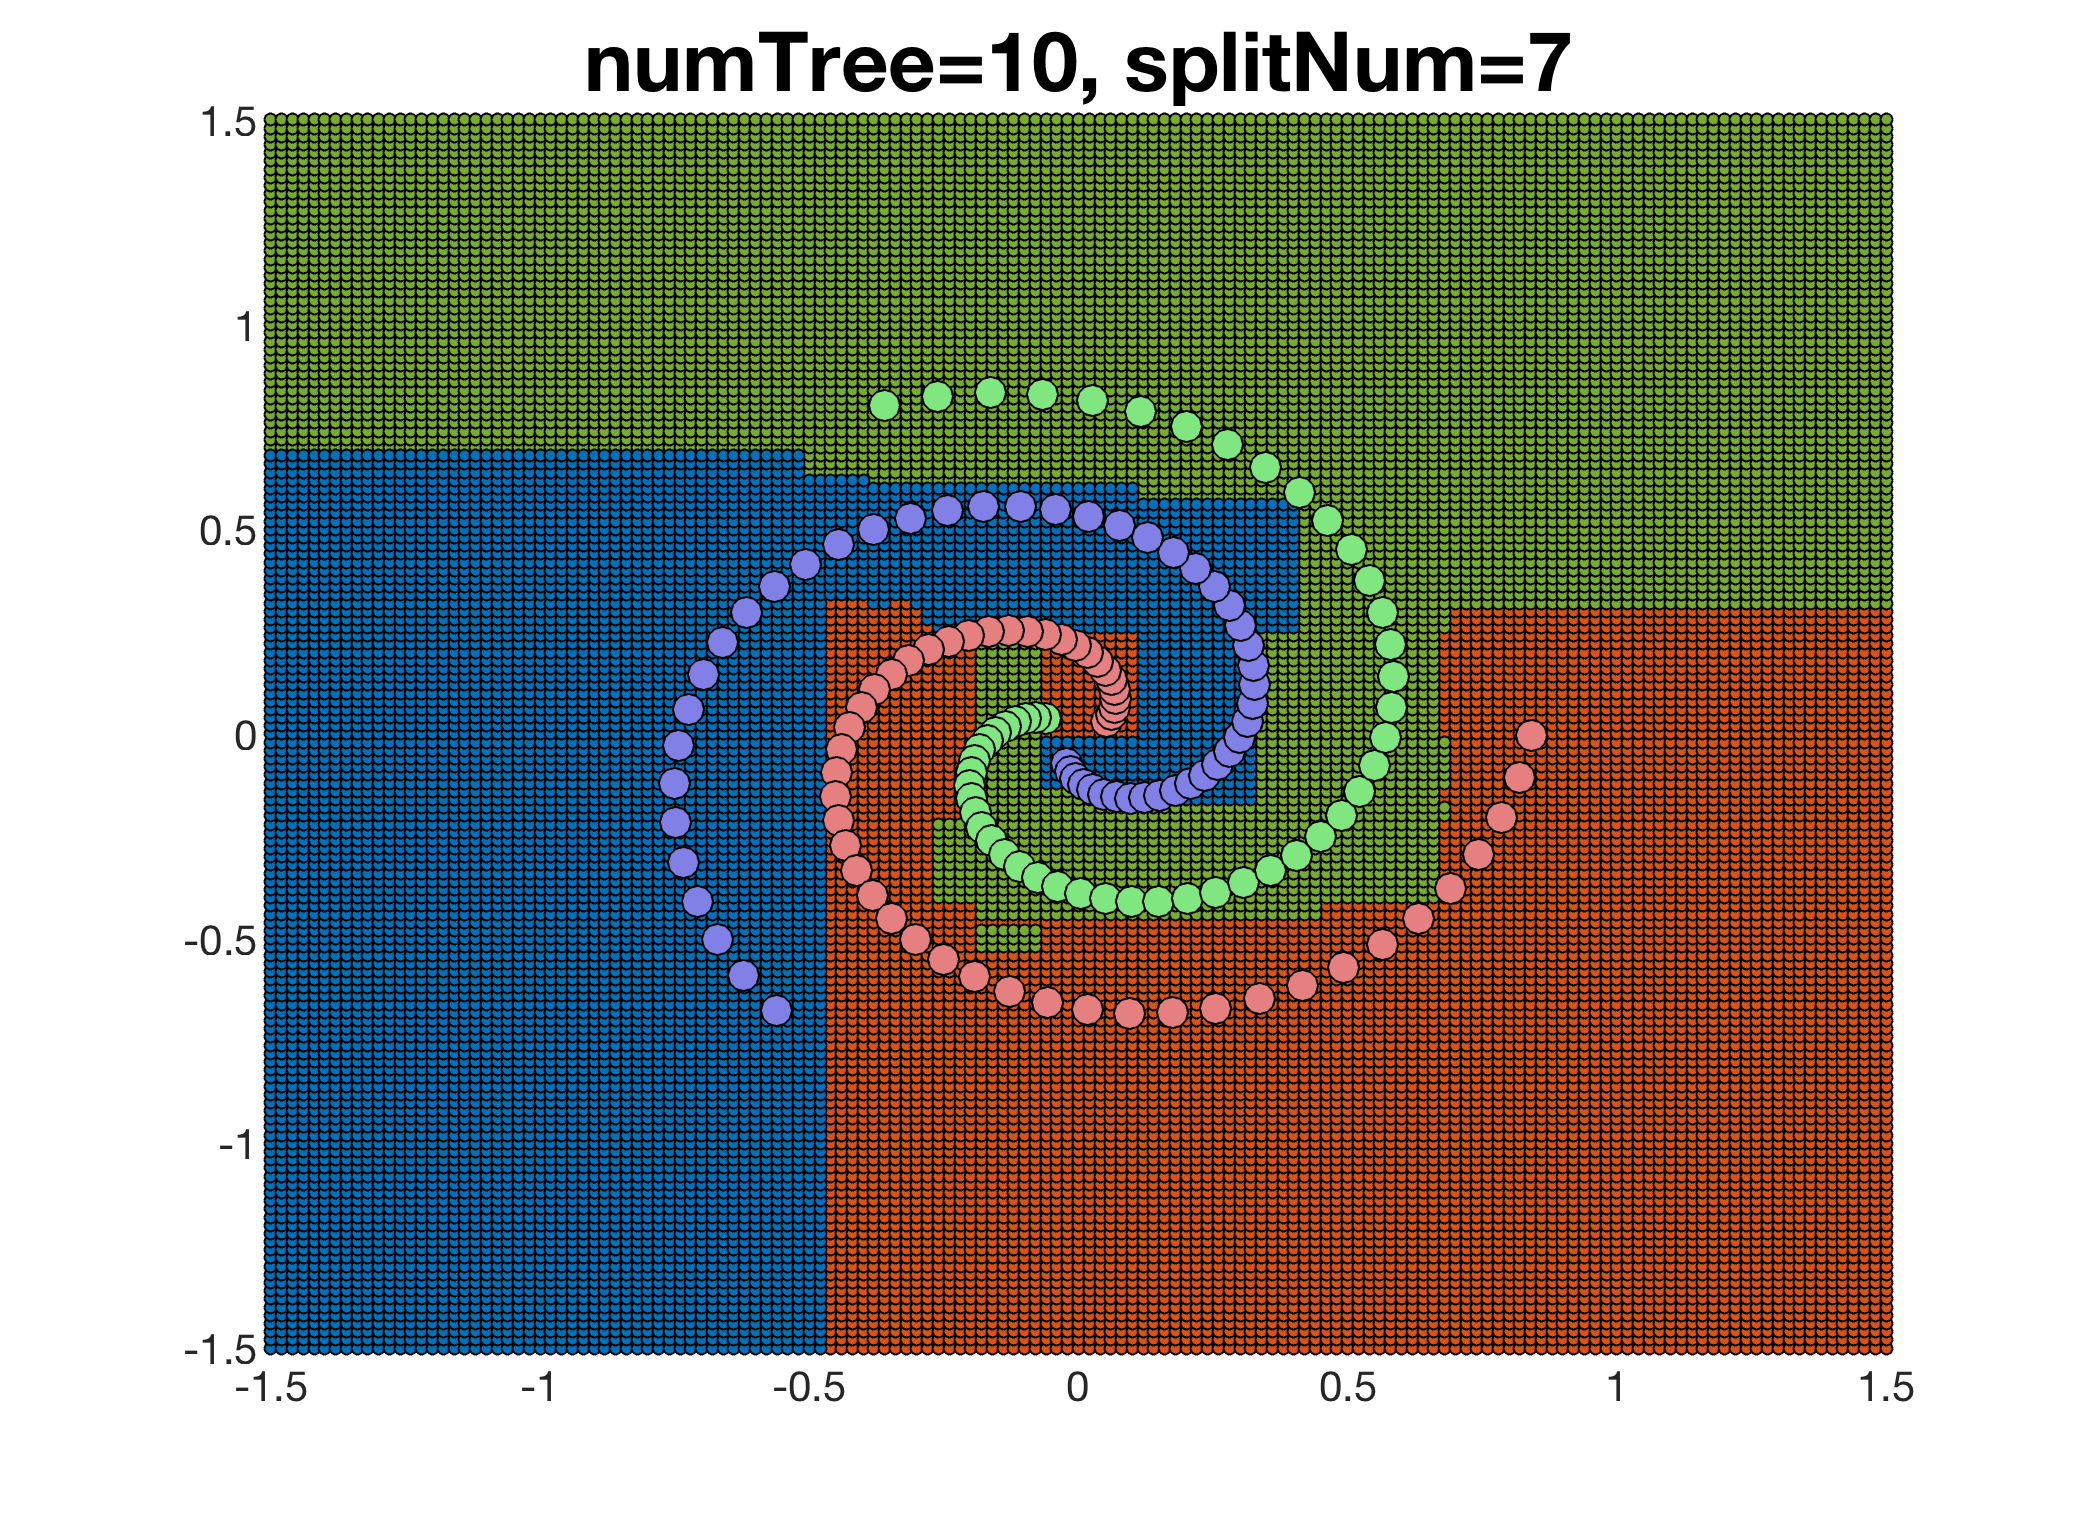
\includegraphics[width=0.40\columnwidth]{splitNum_7}
    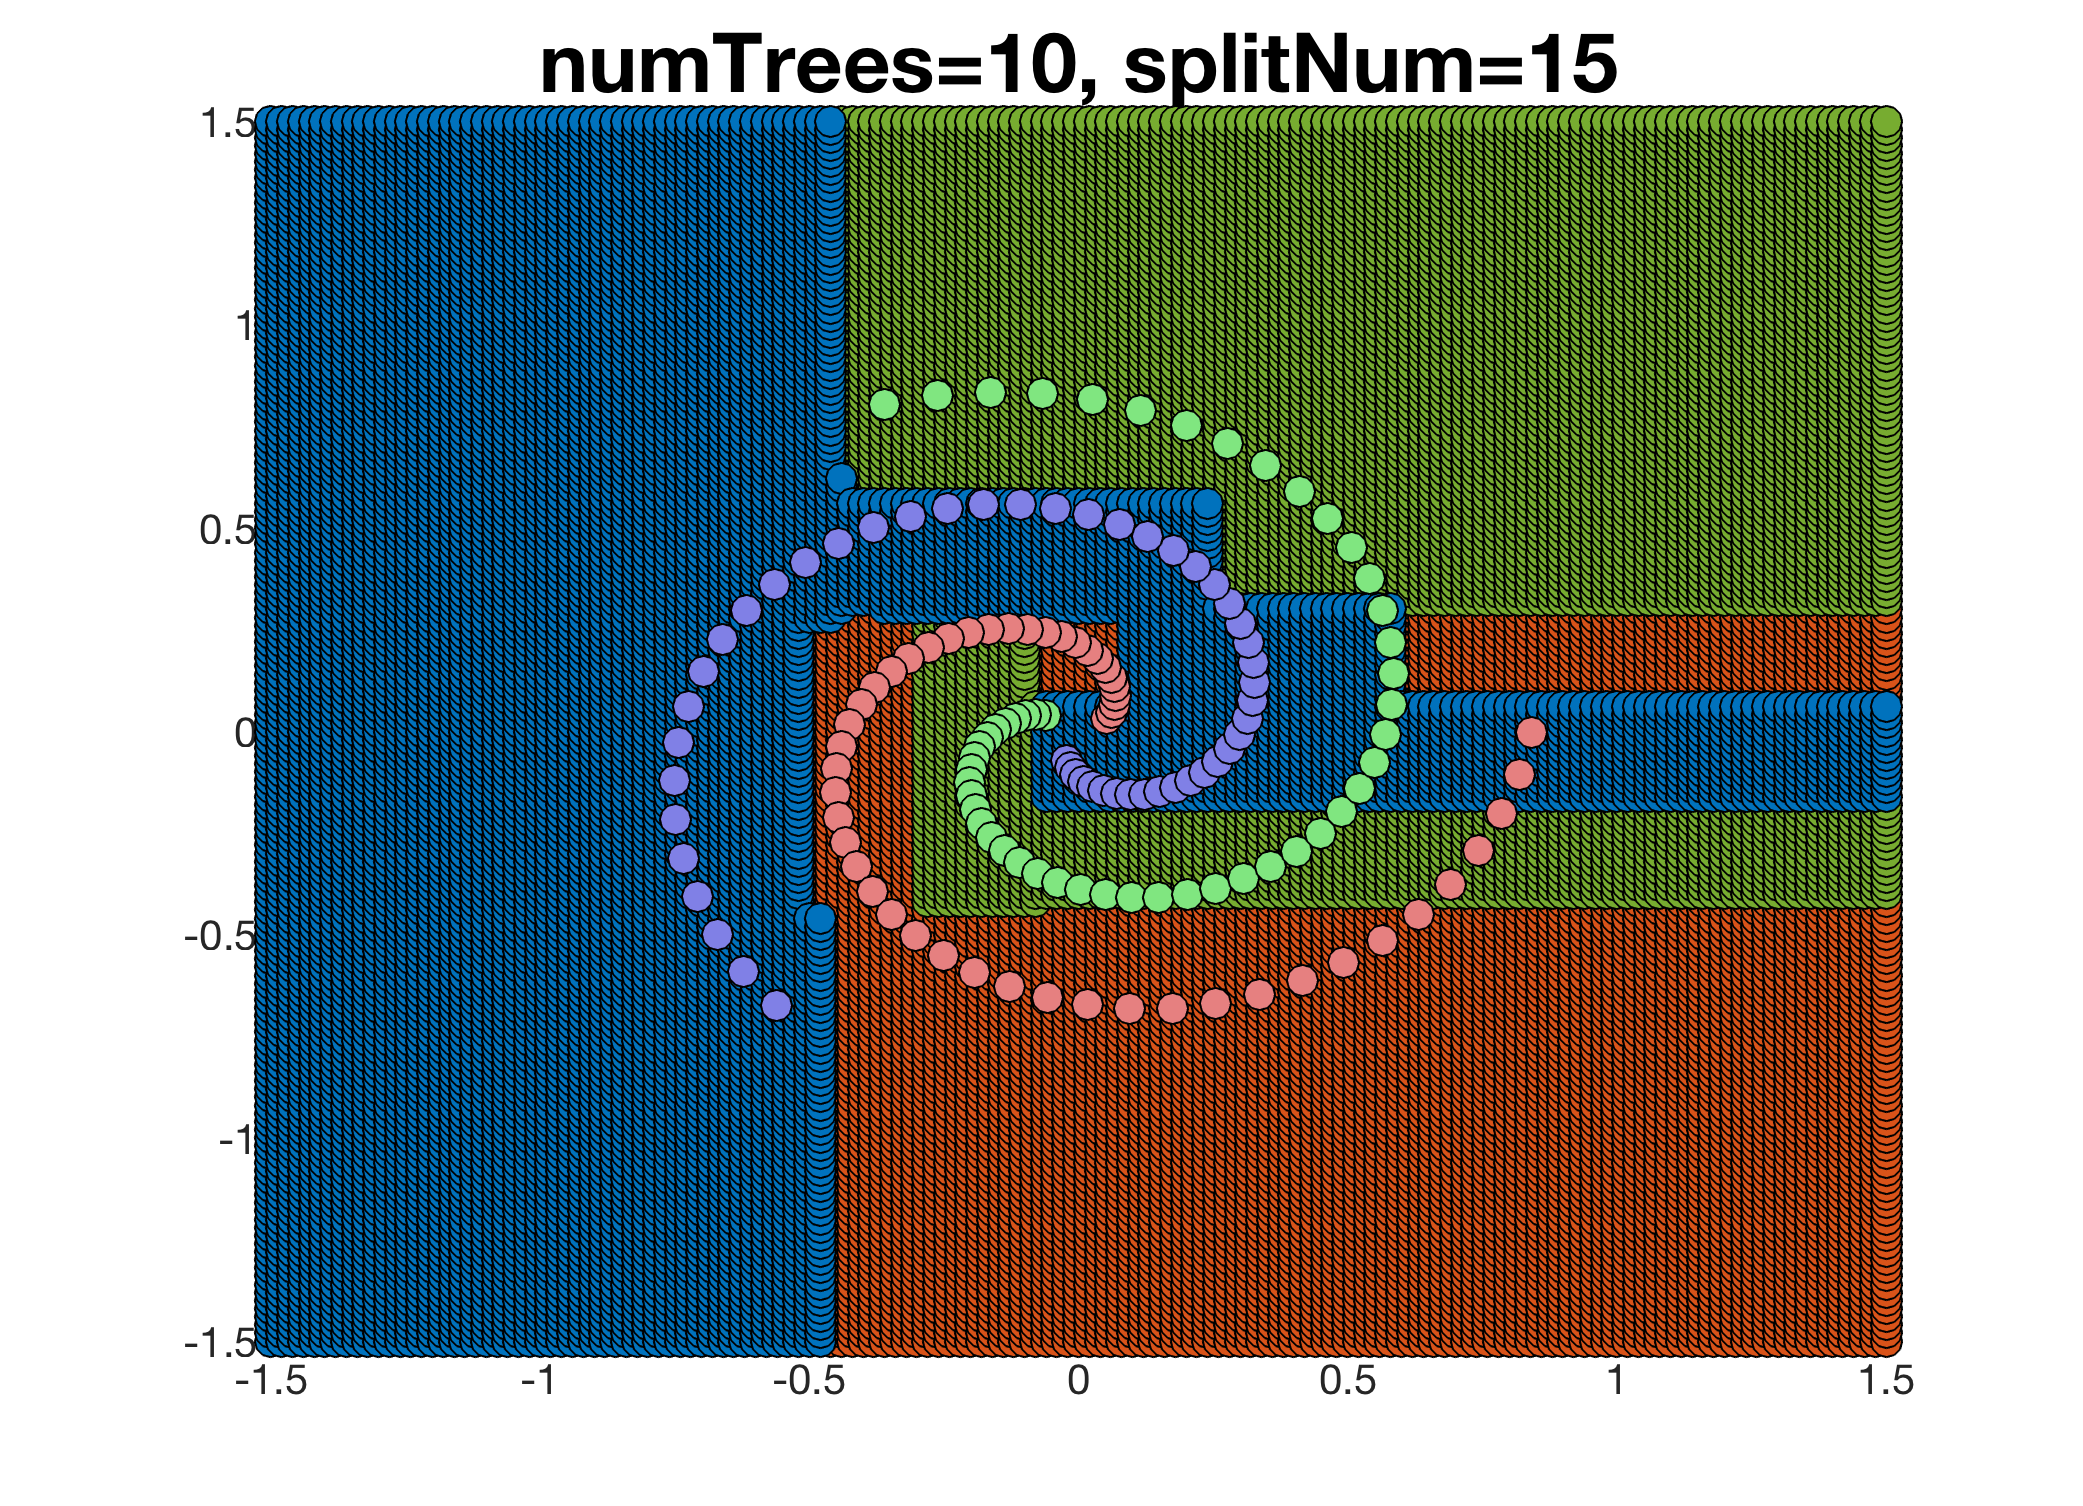
\includegraphics[width=0.40\columnwidth]{splitNum_15}
    \caption{Overview of spectral subtraction process}
\end{figure}

Observe above that with small number of split numbers, artifacts are observed. Each tree is a very bad learner and thus, even though $E_{com}\approx\nicefrac{E_{av}}{T}$, $E_{com}$ is still rather high. Increasing the number of split functions to $7$, the random forest is clearly trying its best to map the spiral nature of the training data using axis-aligned weak-learners. Setting \texttt{param.splitNum} to 15, not only is each tree highly over-fitted, each tree is also highly correlated and thus with only 10 trees, the committee machine cannot sufficiently average away the over-fitting artifacts.

\subsection{Varying Tree Depth}

The third parameter that can be varied is the depth of the tree. More accurate results are produced when tree depth is increased. With depth set at 3 or 5, there are very obvious artifacts that appear; a thin red line when depth is set at 3, and a massive blue region when the depth is set at 5. These are clearly anomalies that have come about because the tree does not sufficiently refine the training data. Increasing the depth to 7, the obvious anomalies have now disappeared but small artifacts still remain at the center of the graph. Results are further improved if the tree depth is increased to 9. 

Tree depth should not be increased arbitrarily for two reasons. As we descend down the tree, training points become refined and get clustered together. If we arbitrarily keep increasing the depth, we will be attempting to separate points which lie very close to one another. Each node's weak-learner has an effect over the entire range of values for which the algorithm is used. Observe what happens when we train on very few number of points in Figure \ref{fig:learners_2}.

Secondly, computational complexity scales exponentially with tree depth. It is much wiser to average out anomalies by increasing the number of trees; while trees can be trained and tested in parallel, each individual tree must be grown sequentially.

\begin{figure}[H]
	\centering
    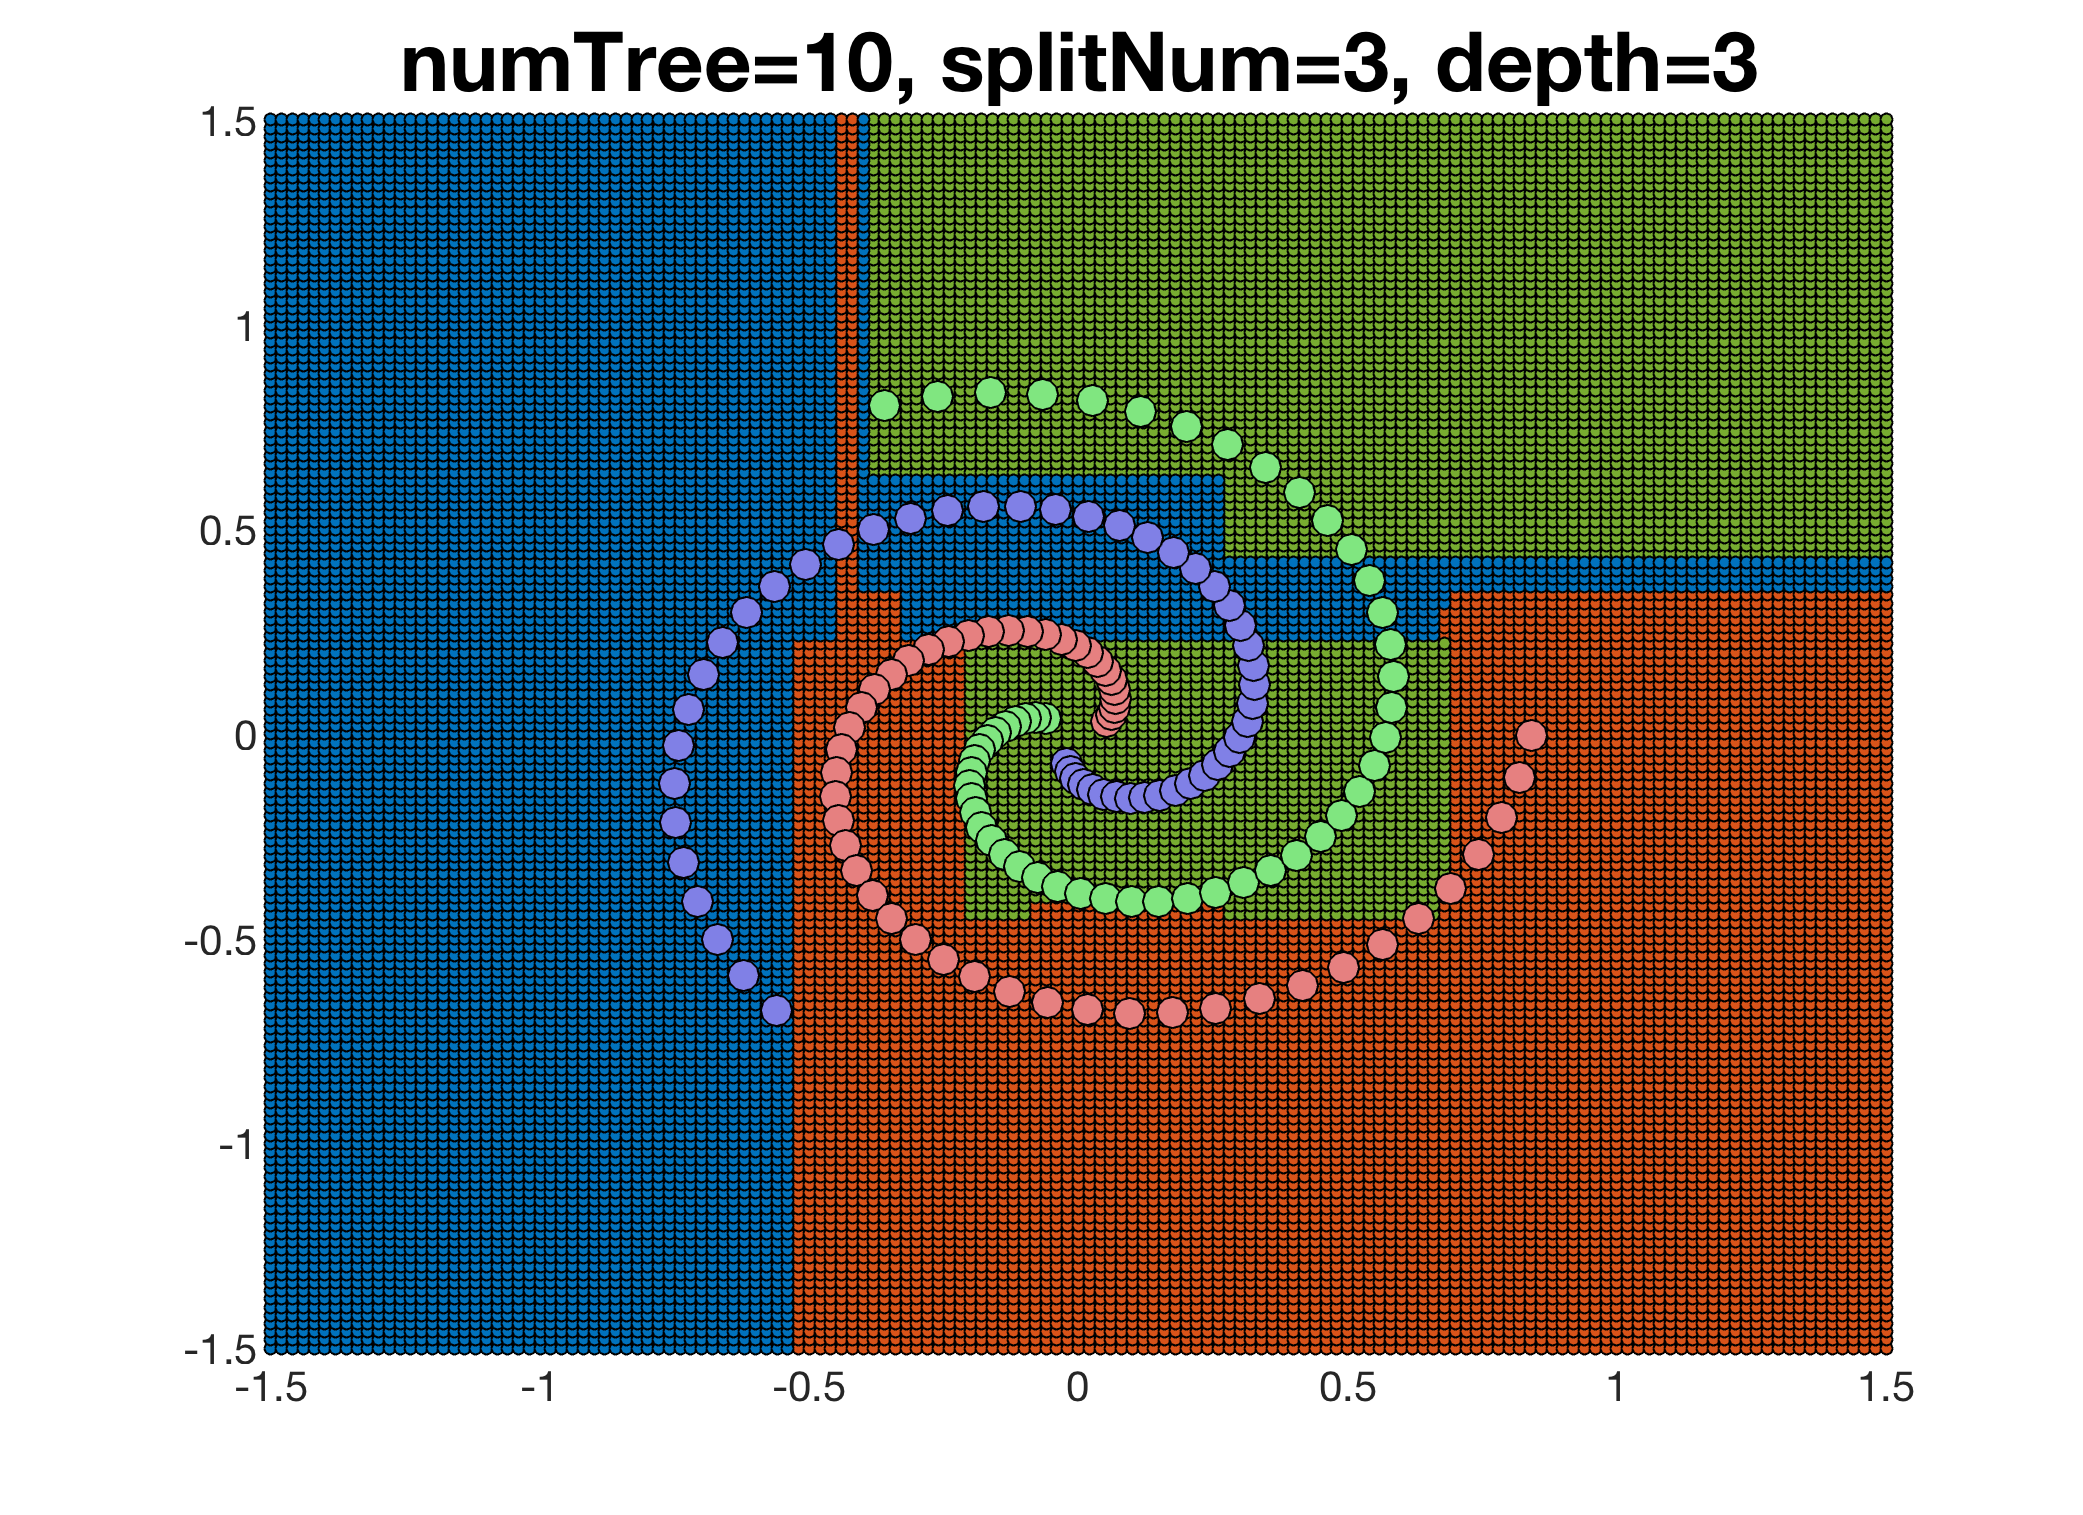
\includegraphics[width=0.40\columnwidth]{tree_depth_3}
	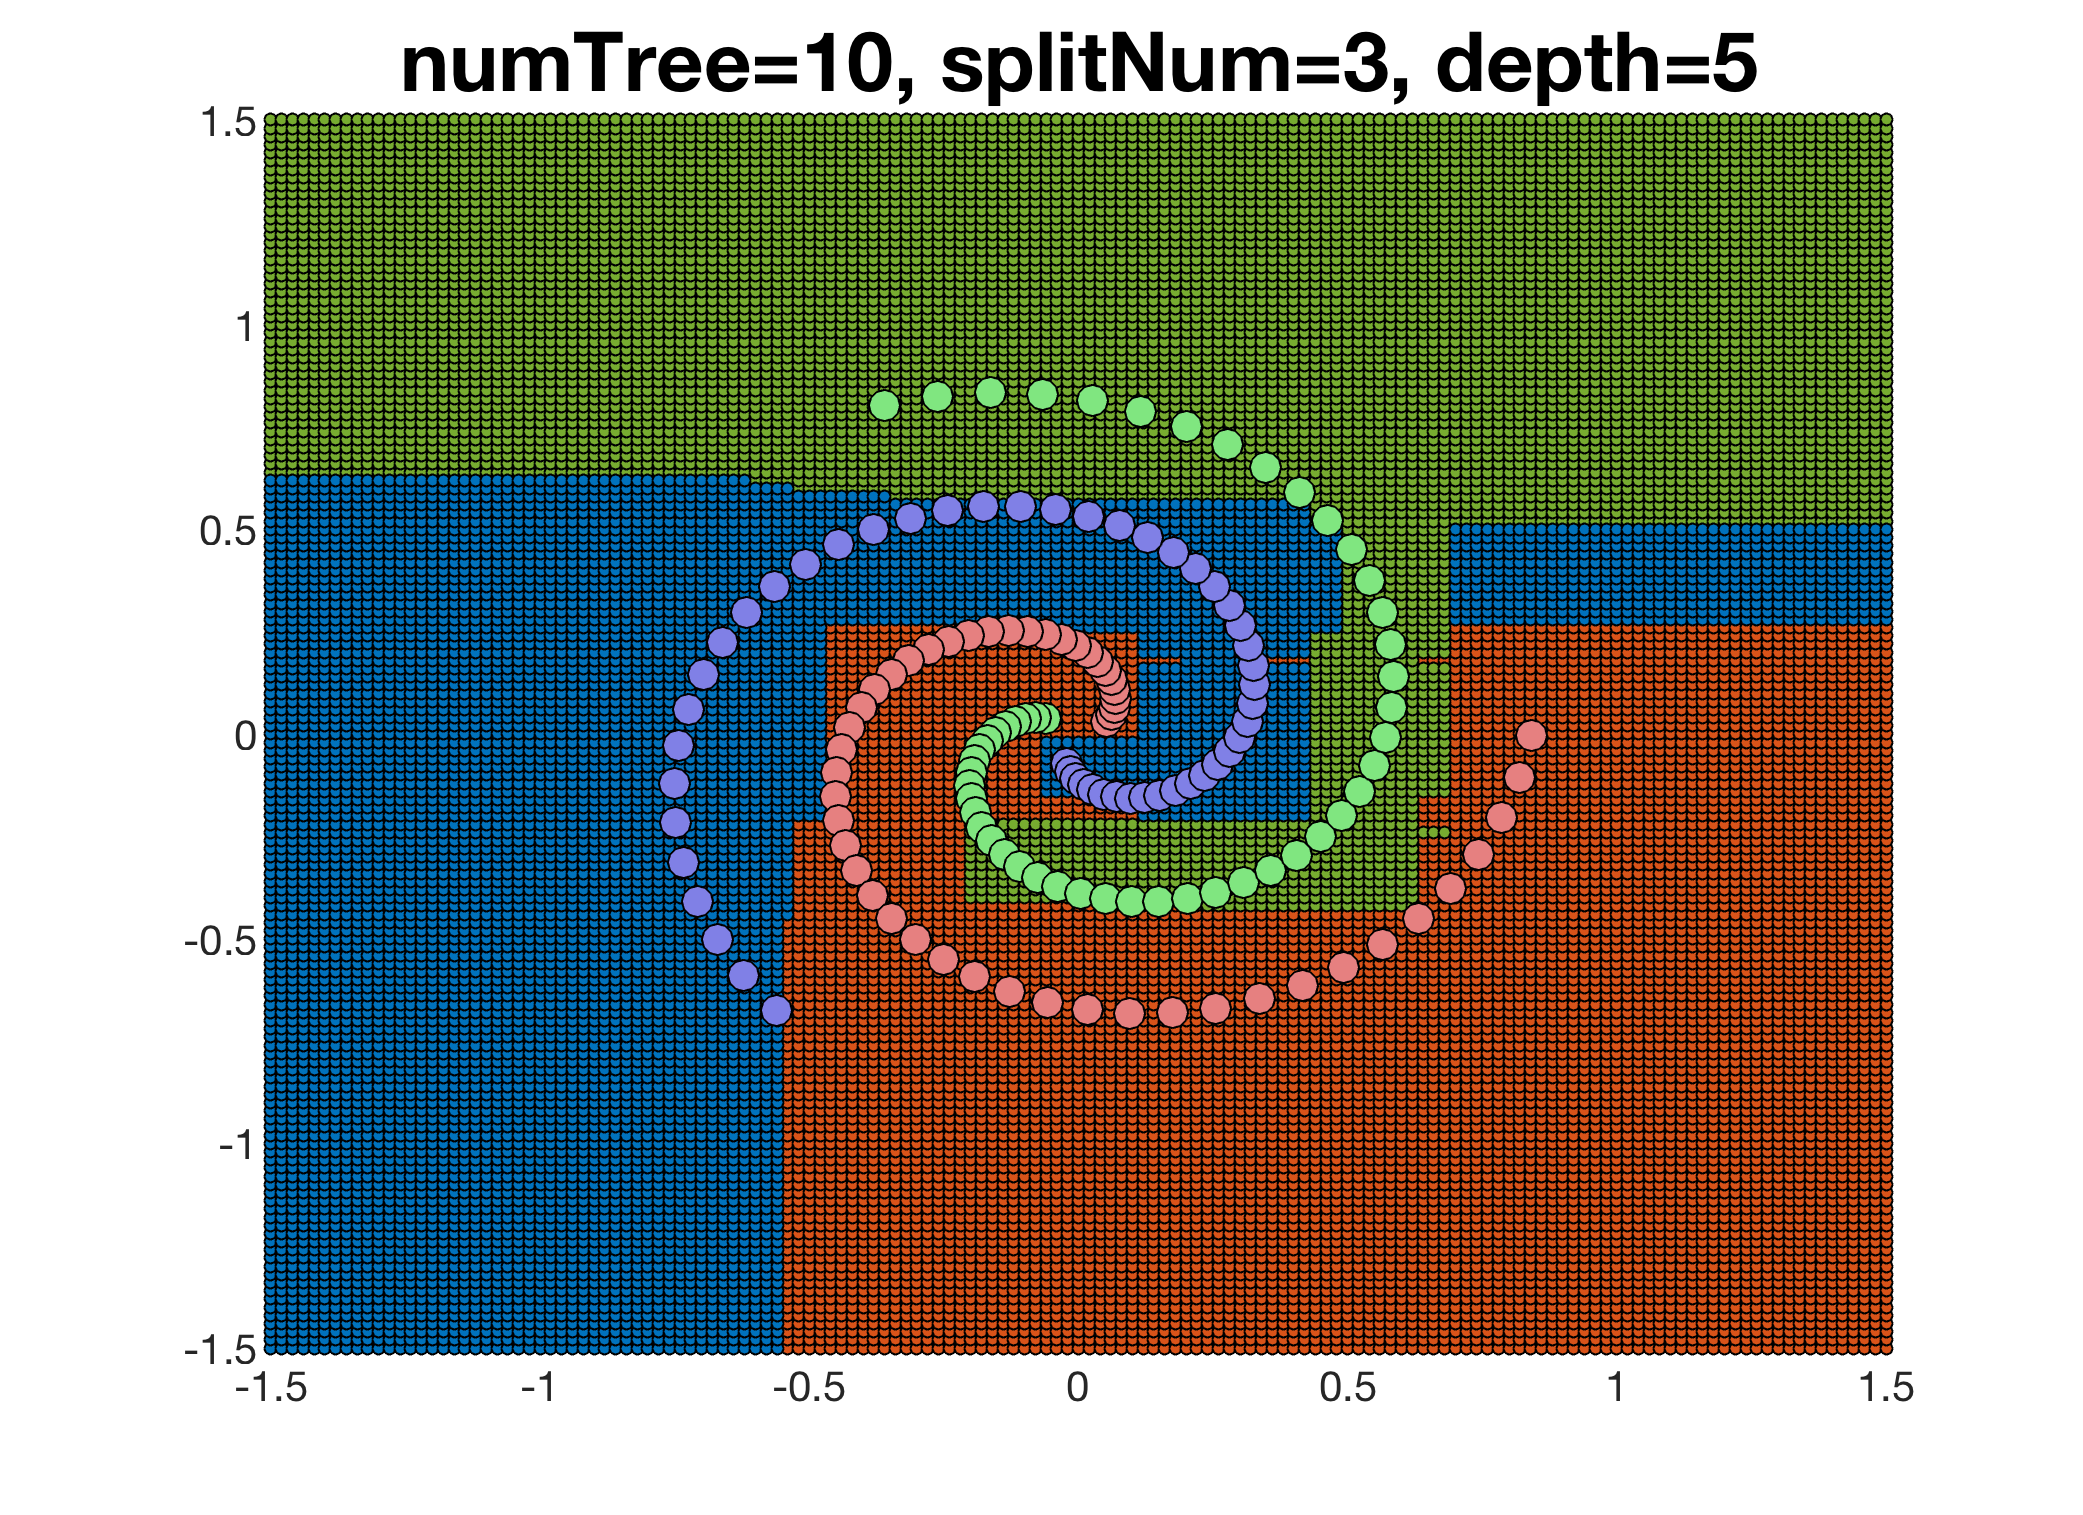
\includegraphics[width=0.40\columnwidth]{tree_depth_5}
    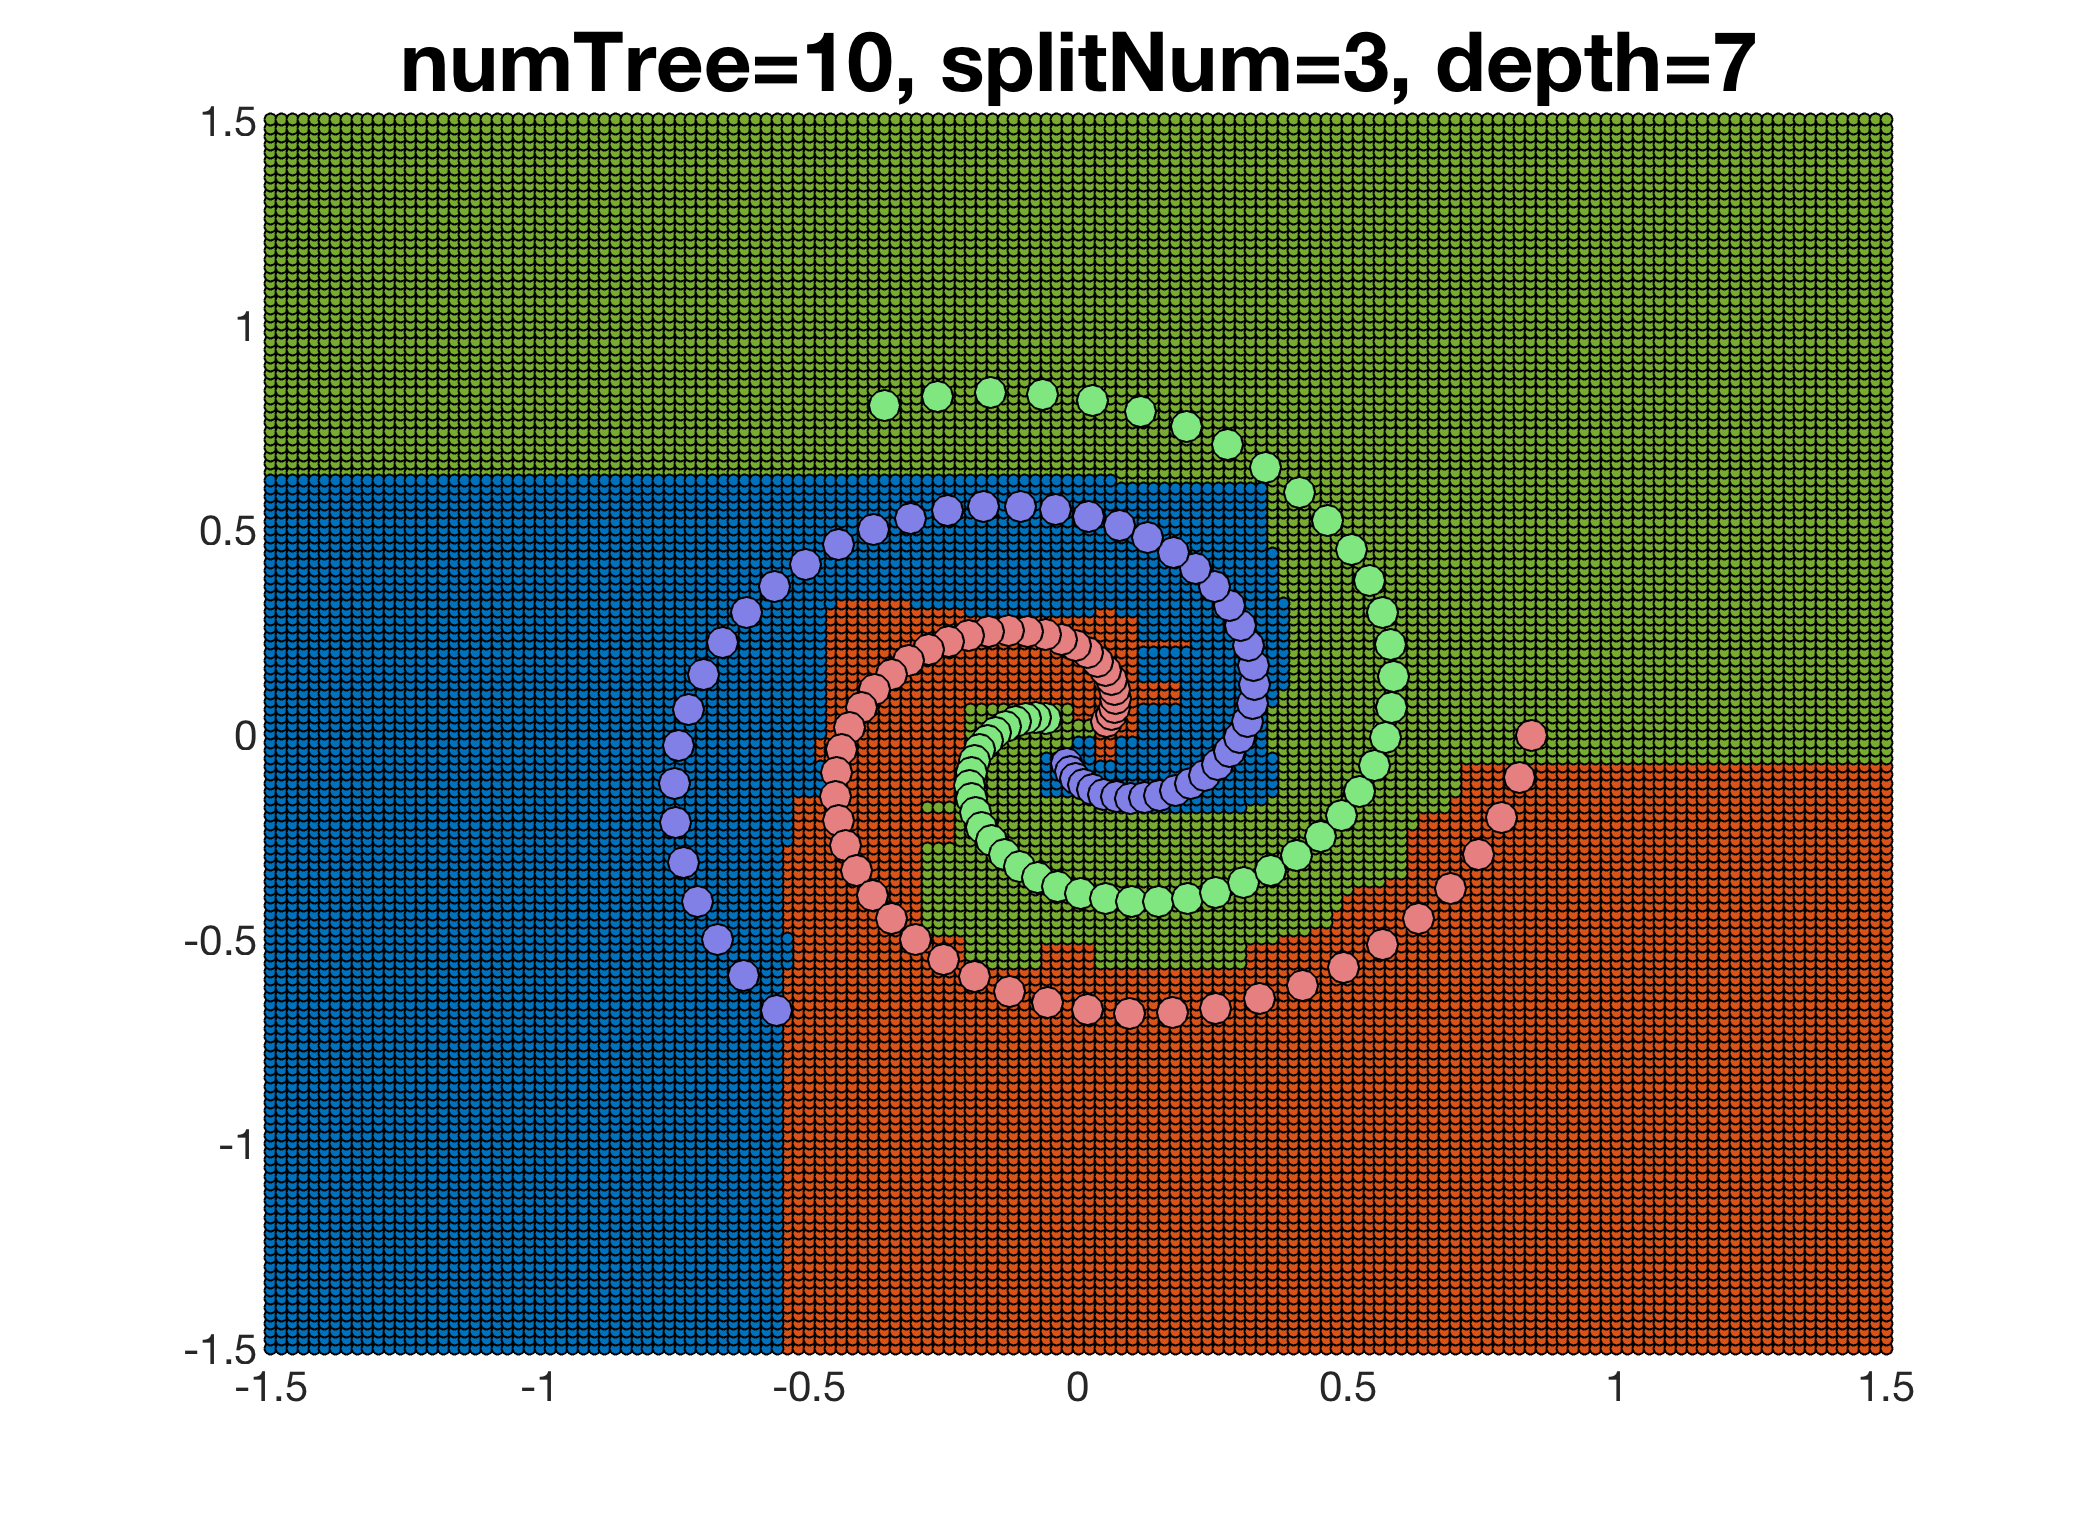
\includegraphics[width=0.40\columnwidth]{tree_depth_7}
    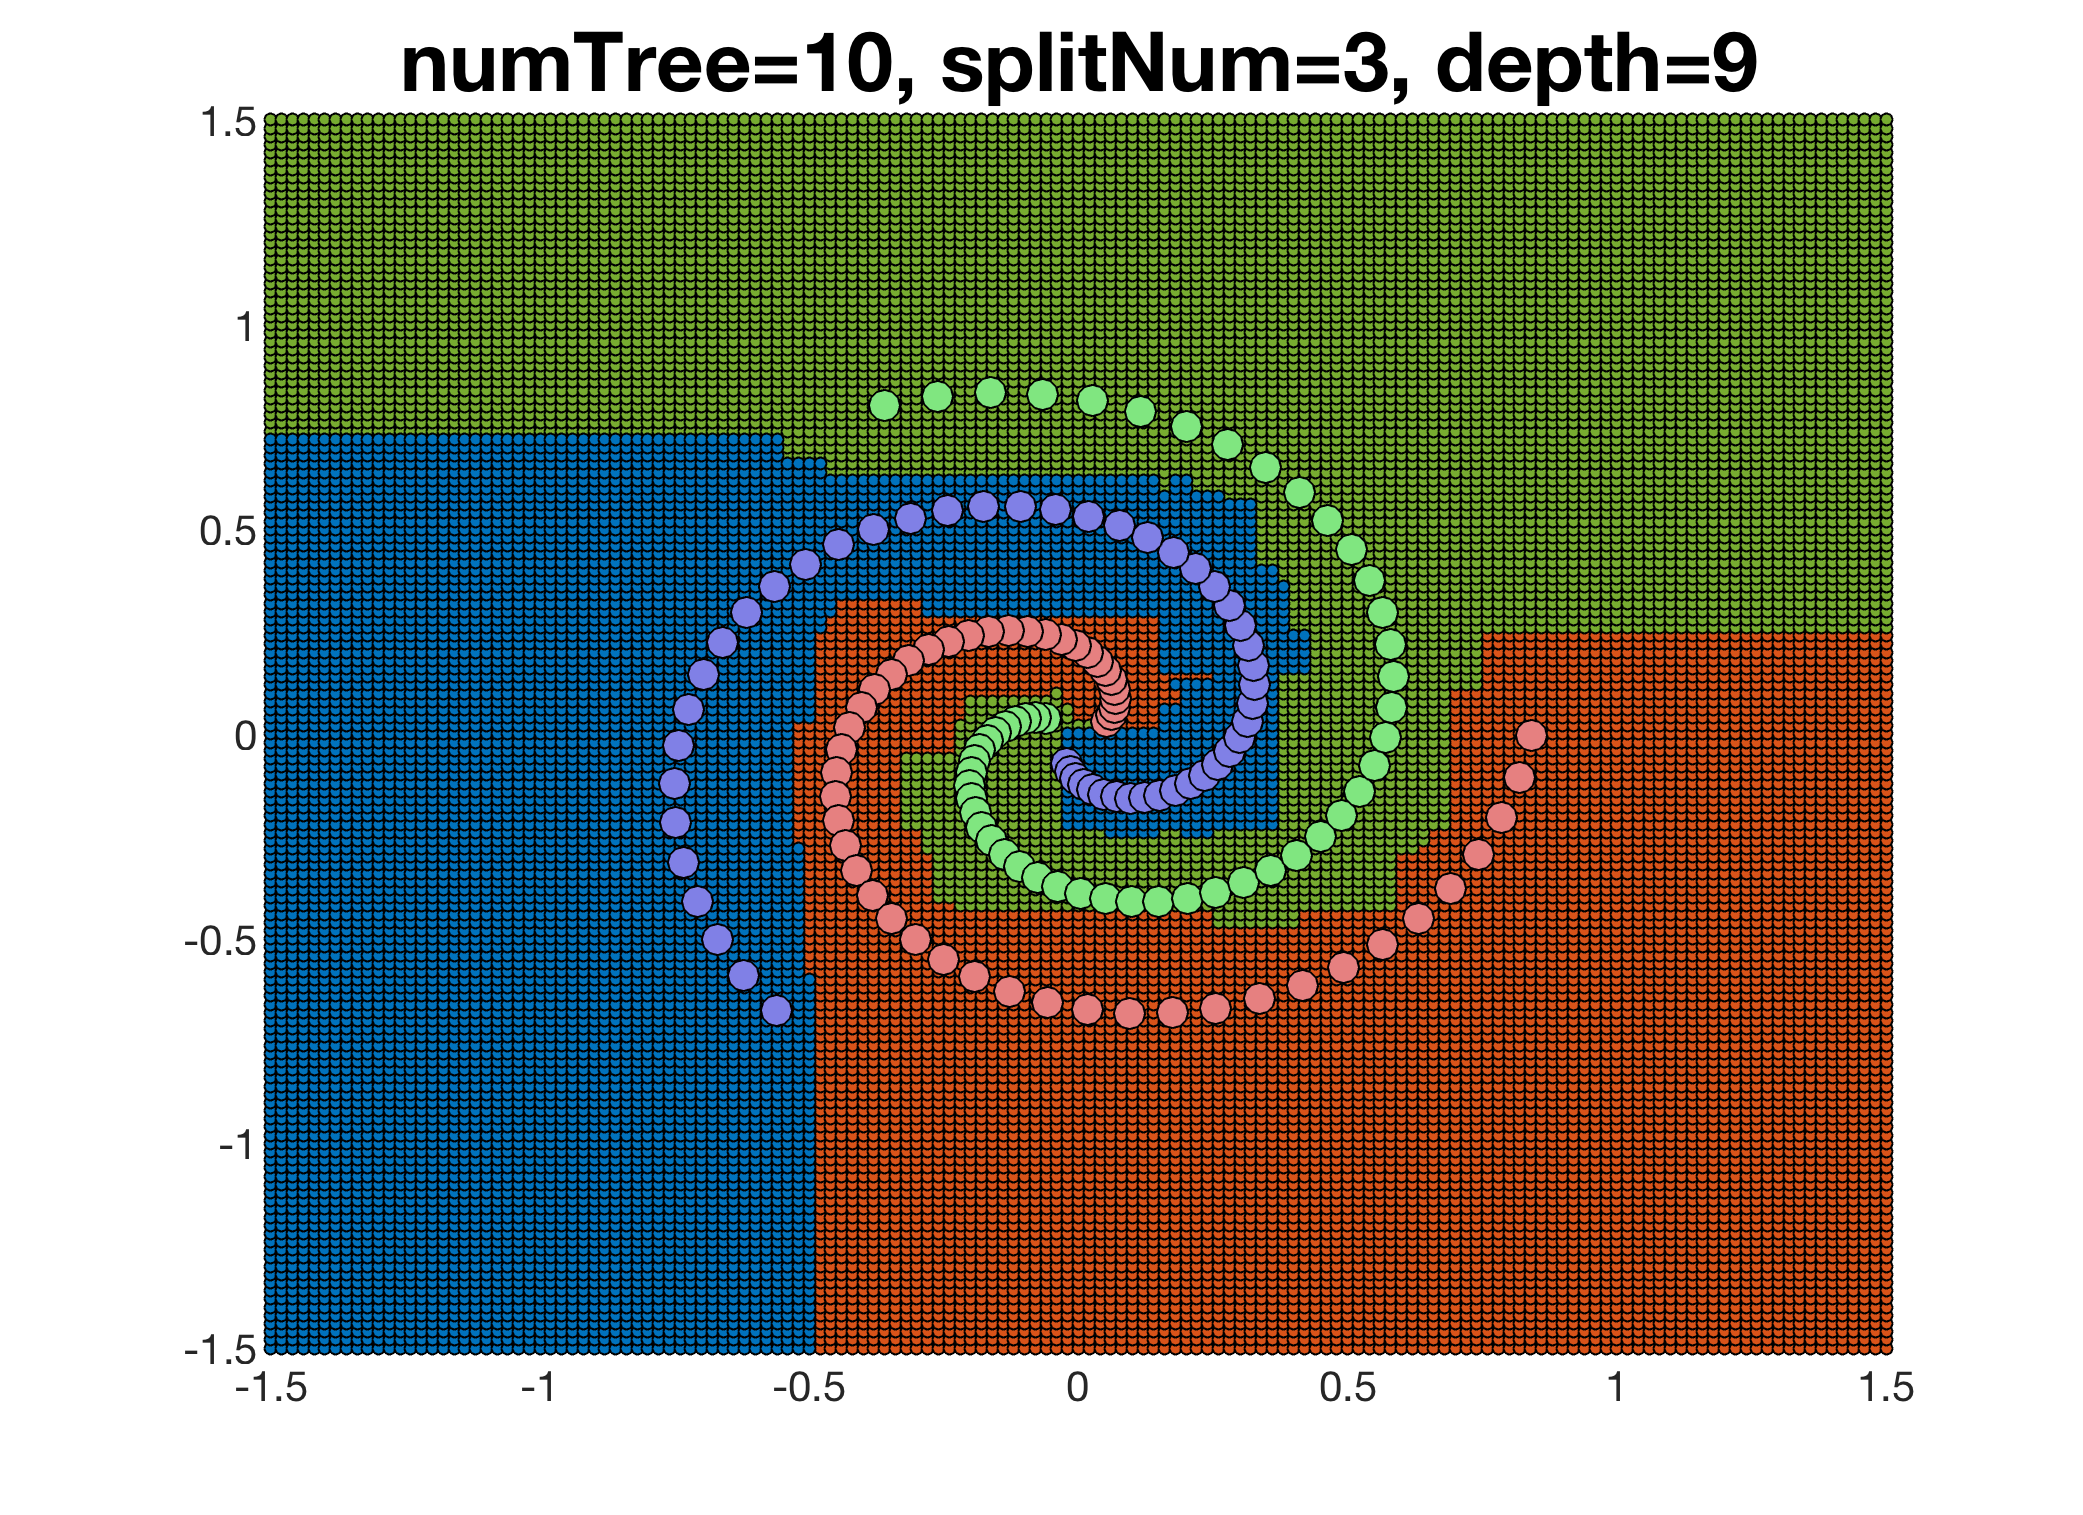
\includegraphics[width=0.40\columnwidth]{tree_depth_9}
    \caption{Overview of spectral subtraction process}
\end{figure}

\subsection{Testing with Different weak-learners}

The entirety of the discussion above has all been made with respect to the axis-aligned weak-learner. The ideal values of random forest parameters very much depend on the class of weak-learner used. The graphs below show the effects of using different weak-learners. The class boundaries in the extrapolated region follow the general shape of the learner class used. For reference, an random forest trained using the axis-aligned weak-learner with all 3 parameters turned has also been graphed.

\begin{figure}[H]
	\centering
    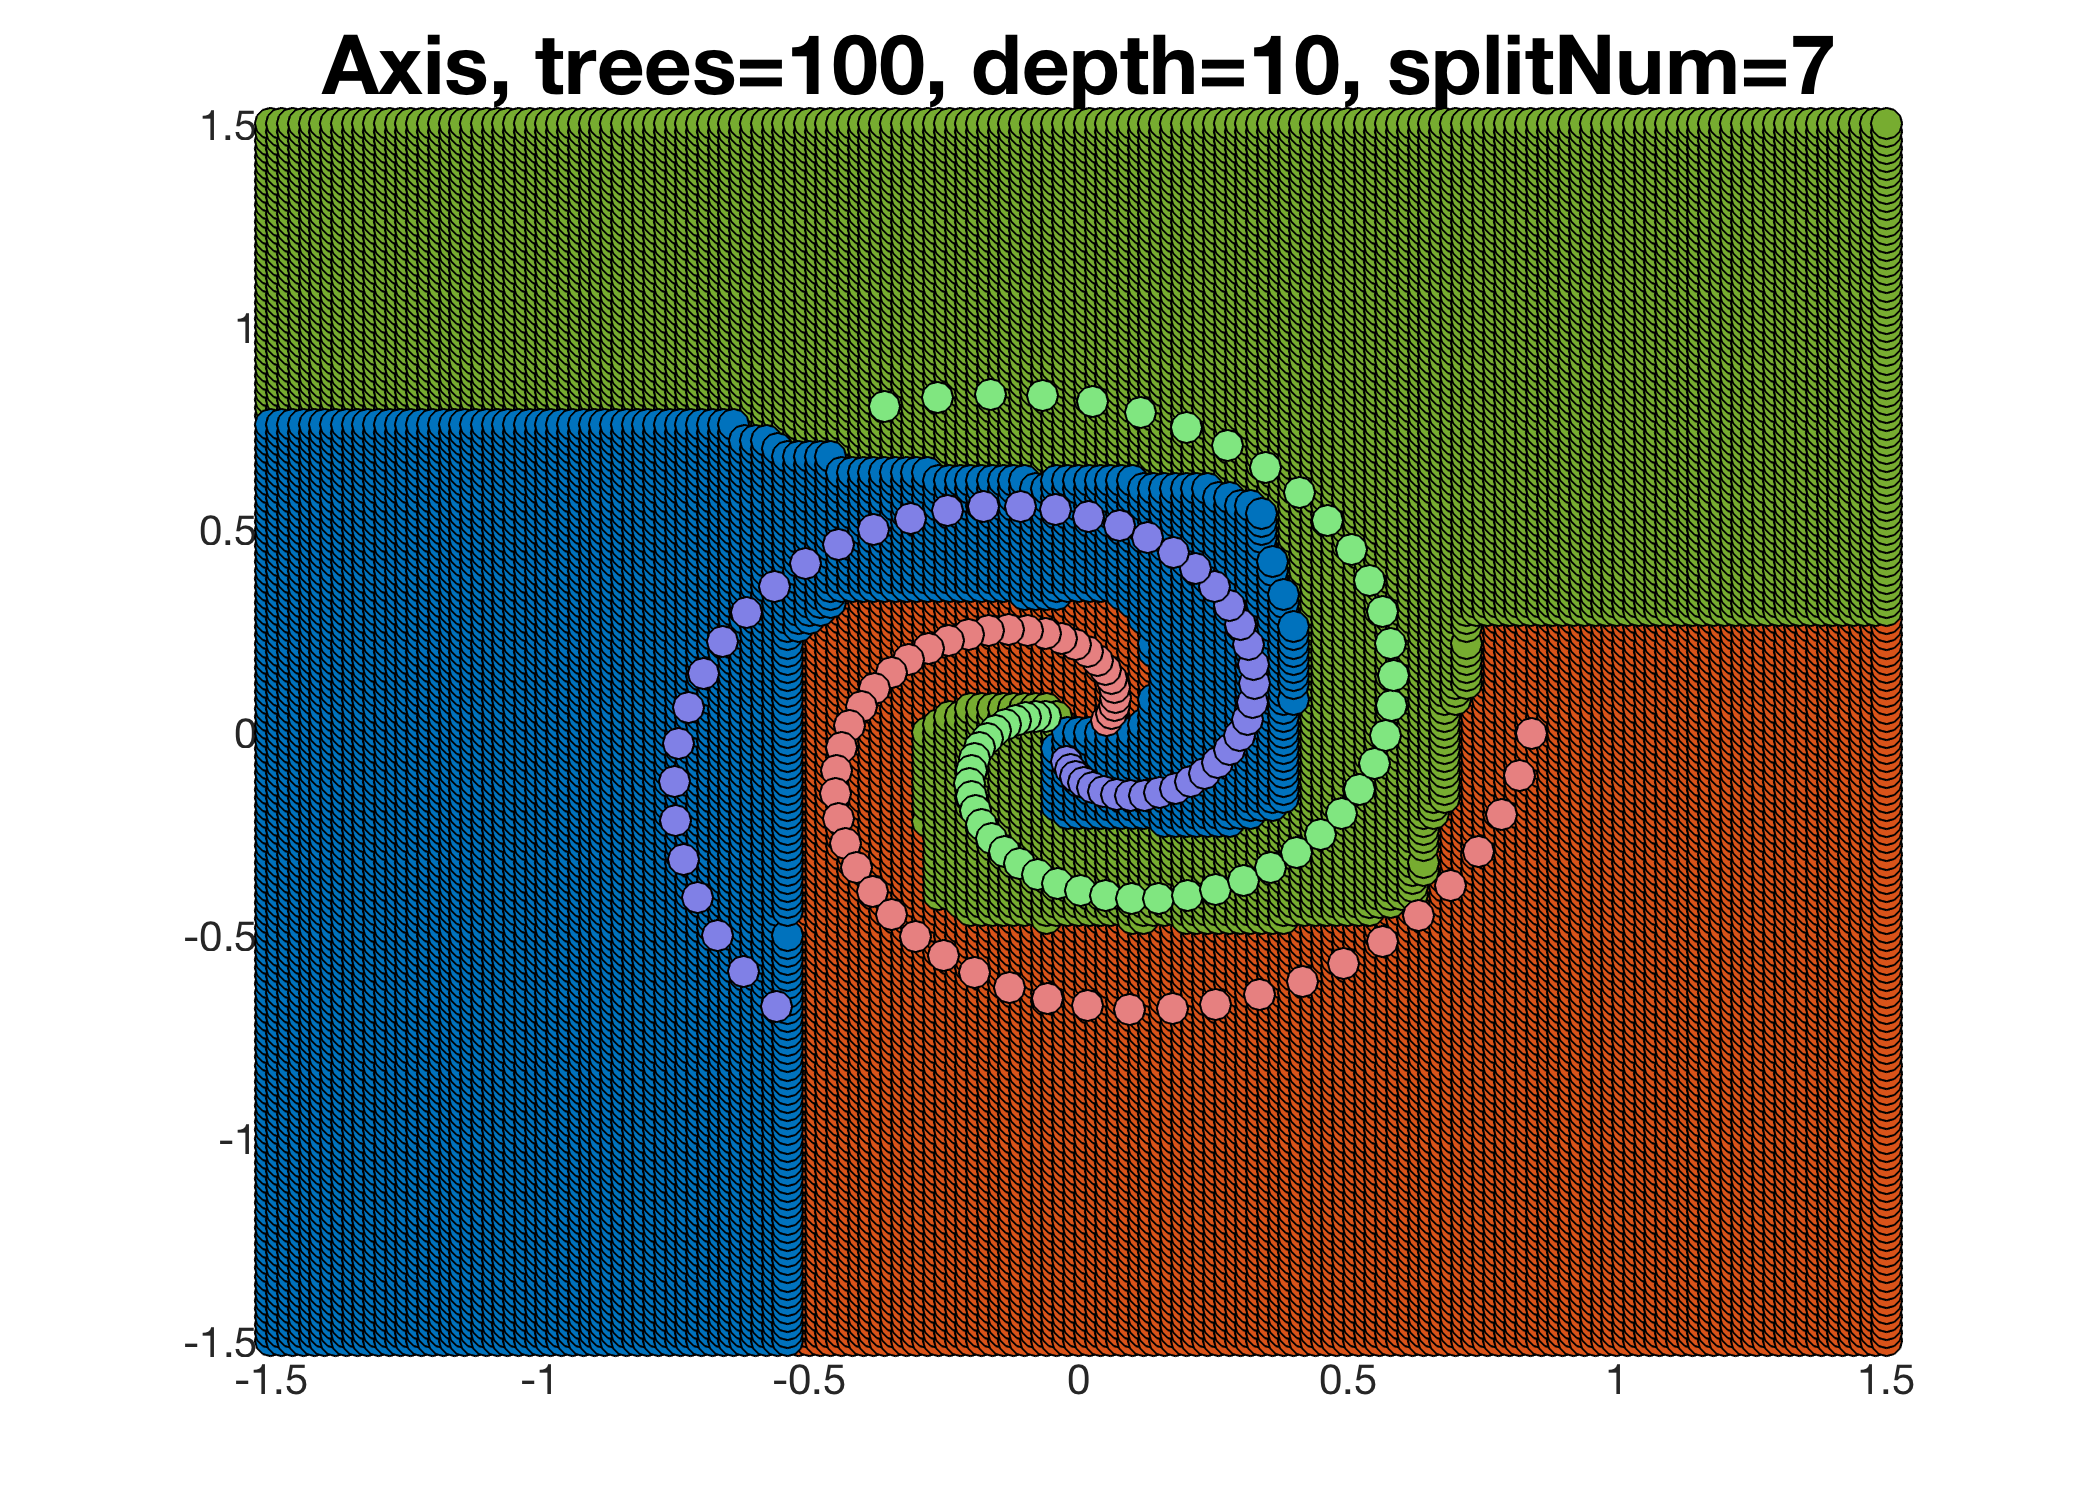
\includegraphics[width=0.40\columnwidth]{axis}
	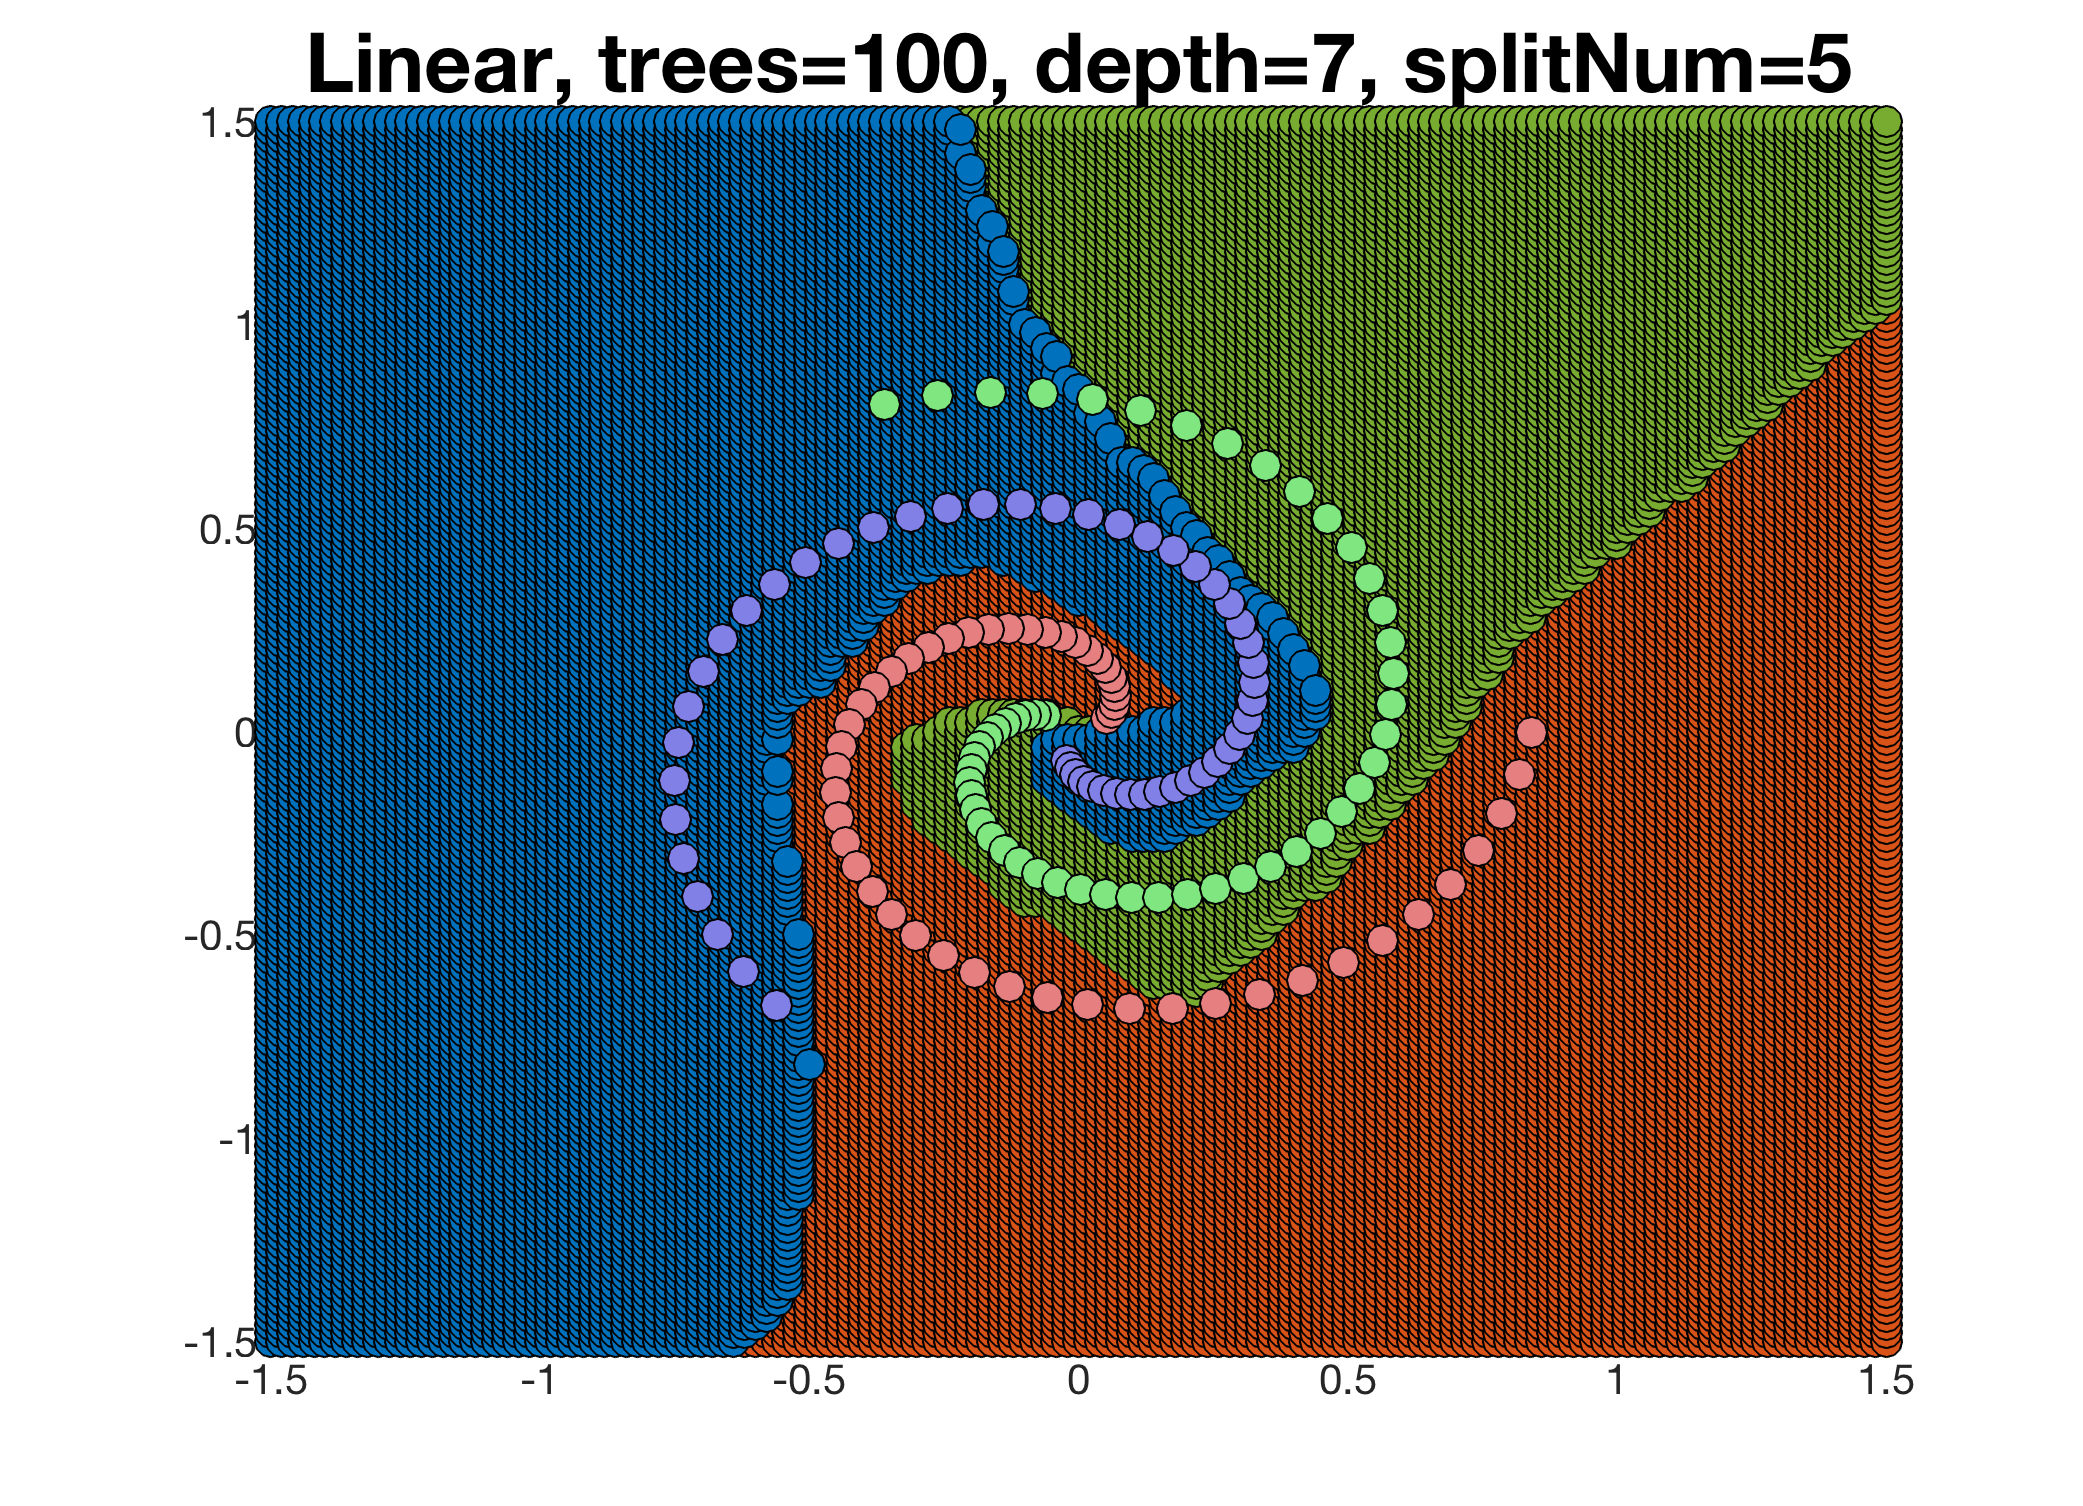
\includegraphics[width=0.40\columnwidth]{linear}
    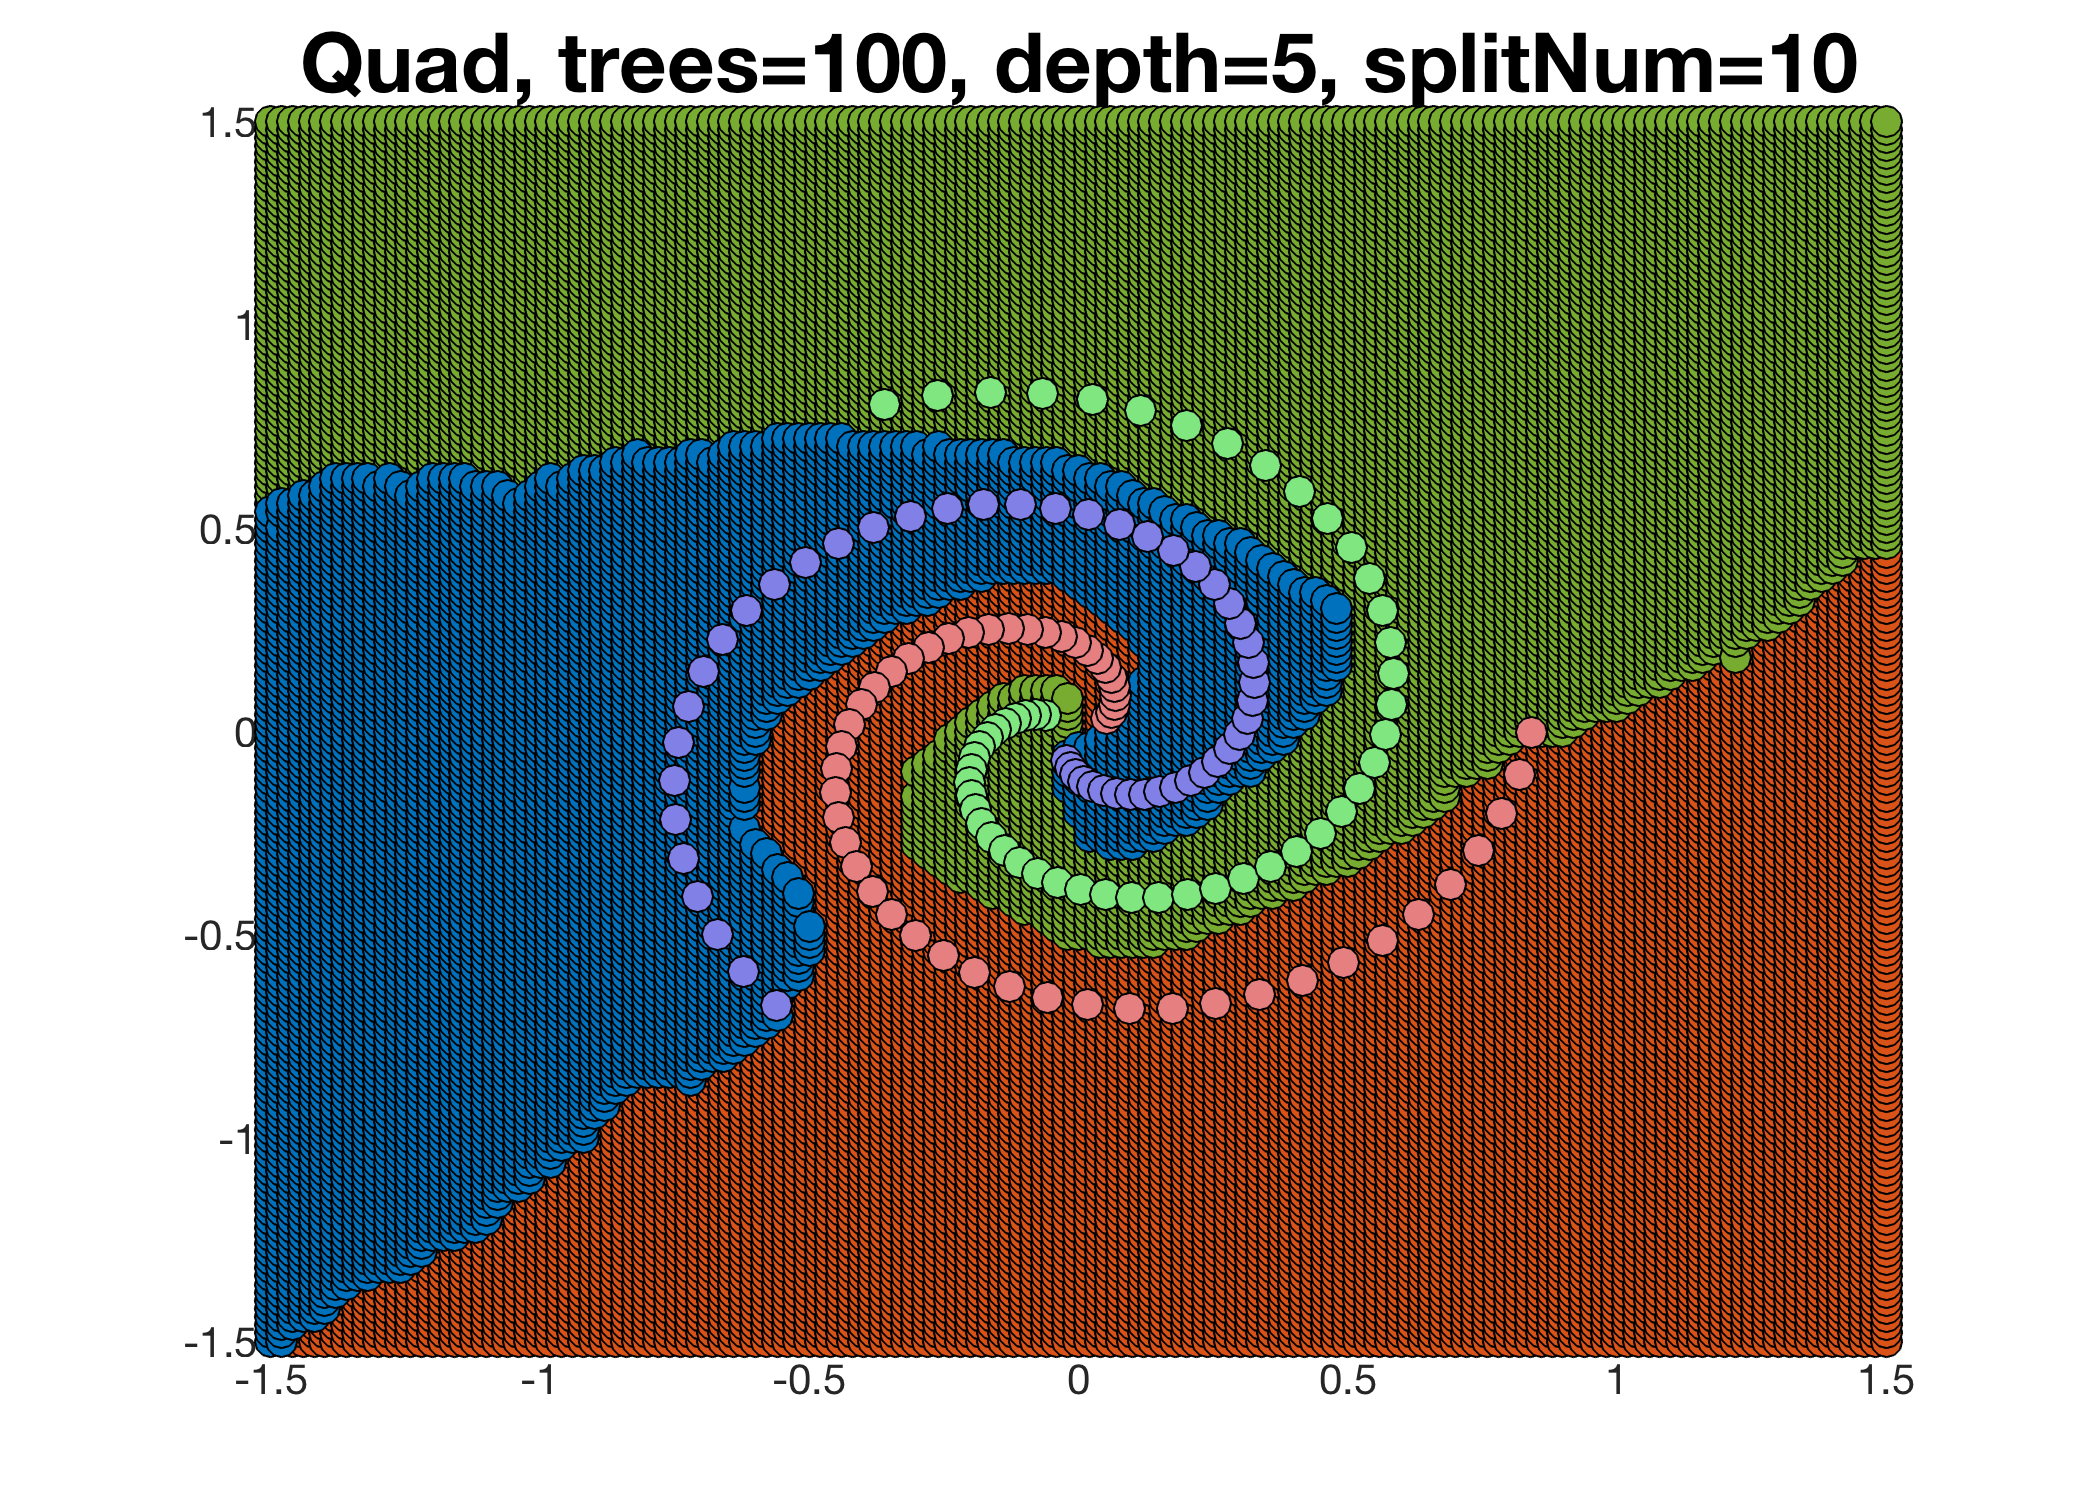
\includegraphics[width=0.40\columnwidth]{quad}
    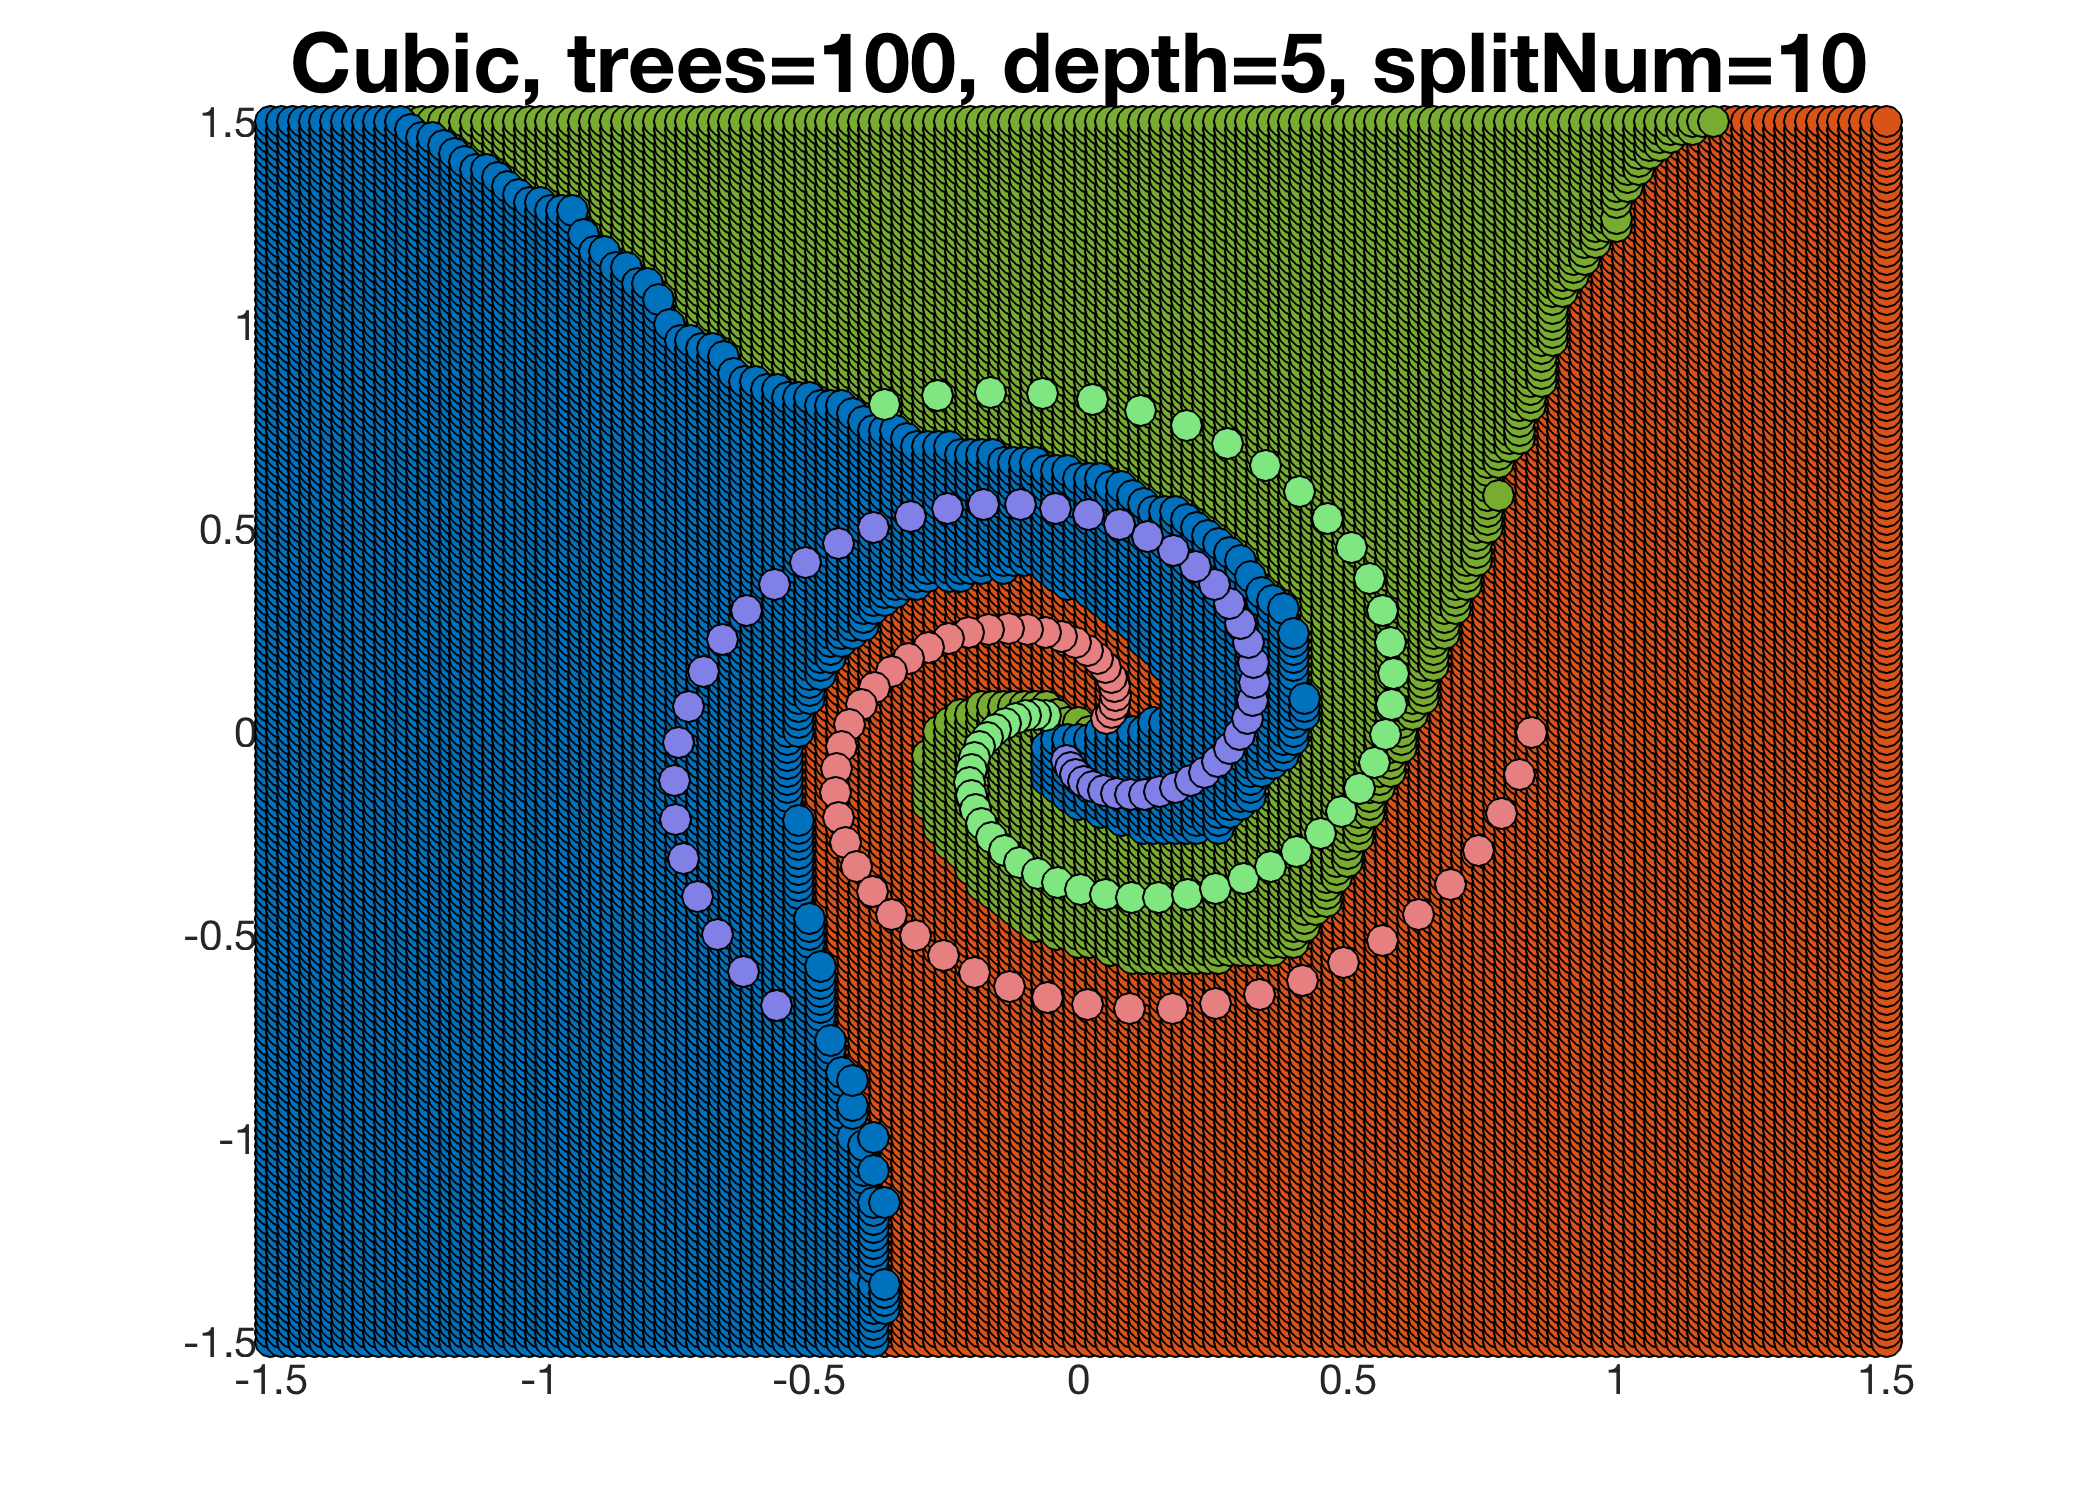
\includegraphics[width=0.40\columnwidth]{cubic}
    \caption{Overview of spectral subtraction process}
\end{figure}


\section{K-means Codebook}

\subsection*{Vocabulary Size}

Using the K-means algorithm to form a Bag-of-Words (BoW) representation, we have direct control over vocabulary size. The vocabulary is going to consist of exactly K codewords. The BoW can be interpreted as a dimensionality reduction technique that shrinks an image into a histogram which indicates the frequency of occurrence of each codewords in our vocabulary. Note that classification is performed using only the histogram and the physical meaning of each codeword is not relevant to the random forest classifier. In fact, more often than not, codewodes do not match heurestic features such as eyes or wheels. With that in mind, it should be noted that the performance of the classifier is heavily dependent on richness of the vocabulary. To form the K-means codebook, matlab's inbuilt function \texttt{kmeans} is used; matlab implements the K-means++ algorithm (QUOTE THIS SHIT), which exhibits a complexity of $\mathcal{O}(\text{log} \ \text{K})$.

\subsection*{Vector Quantisation Process}

The first step in the vector quantisation process involves extracting Scale Invariant Feature Transform (SIFT) descriptors for each image in our training dataset. Extraction is performed using the function \texttt{vl\_phow}, which comes with the reference code provided for this coursework. The function outputs 128-dimensional descriptors; note that the number of descriptors returned depends on the image. After obtaining descriptors for each image in the training dataset, 100,000 descriptors are randomly selected to form a intermediate dataset in a 128-dimensional vector space. This intermediate dataset is fed into the K-means algorithm; only 100,000 descriptors are used to place reasonable bounds the computational complexity both in terms of time and memory. The K-means algorithm will return K cluster centers, where K represents the size of our codebook.

\begin{figure}[H]
	\centering
    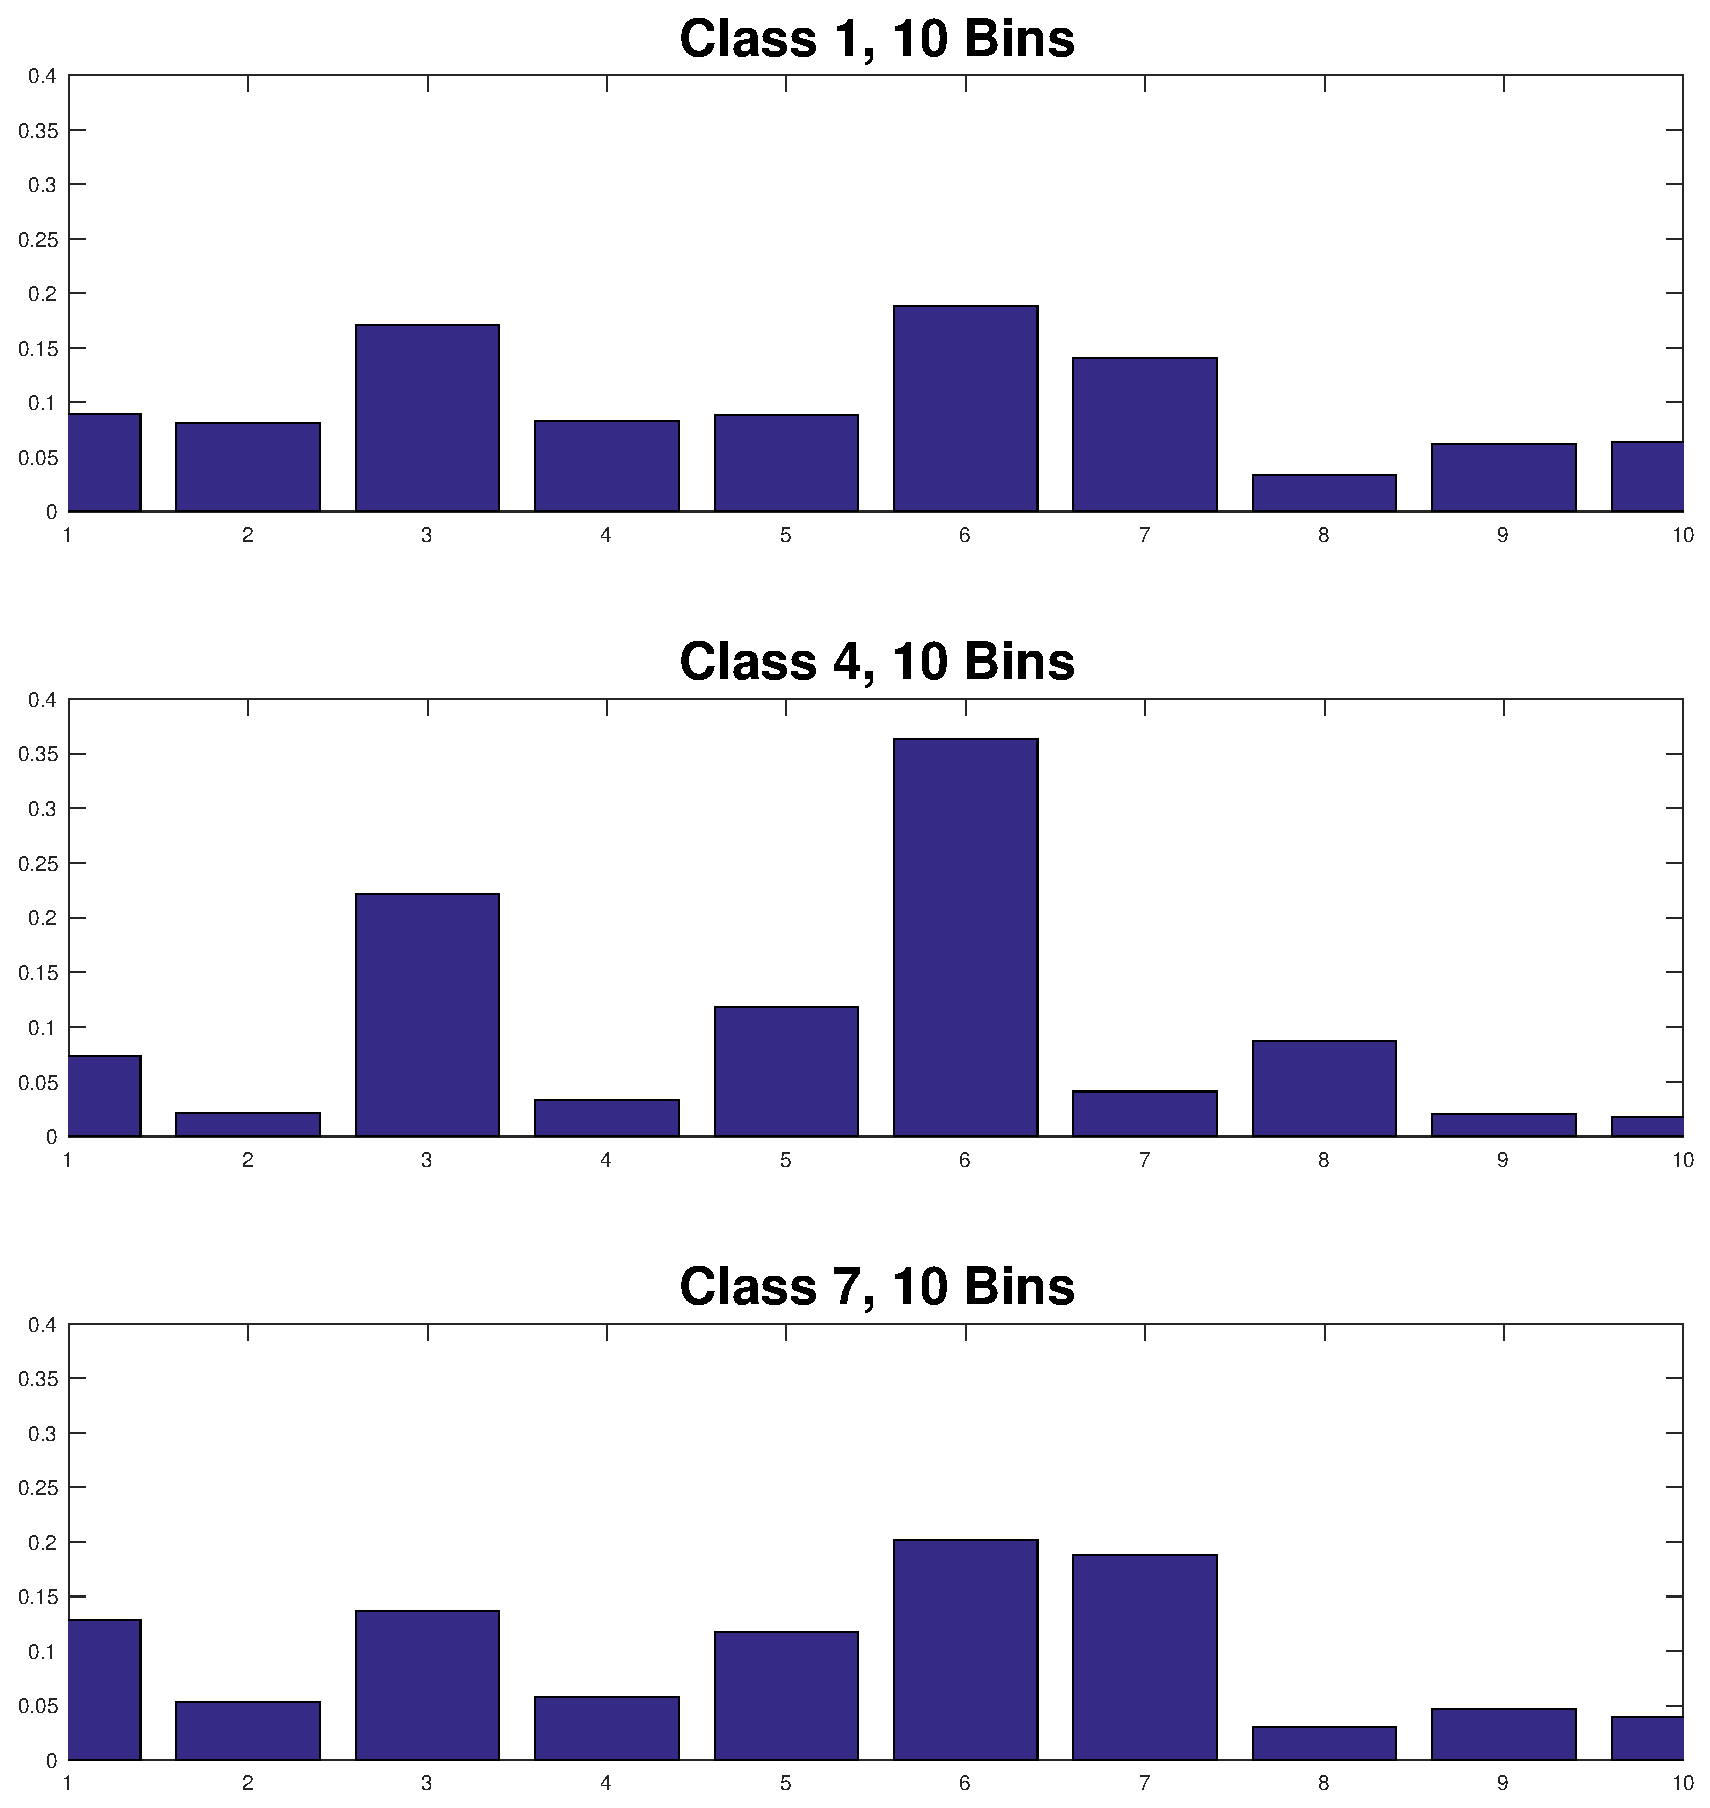
\includegraphics[width=0.49\columnwidth]{hist_10}
    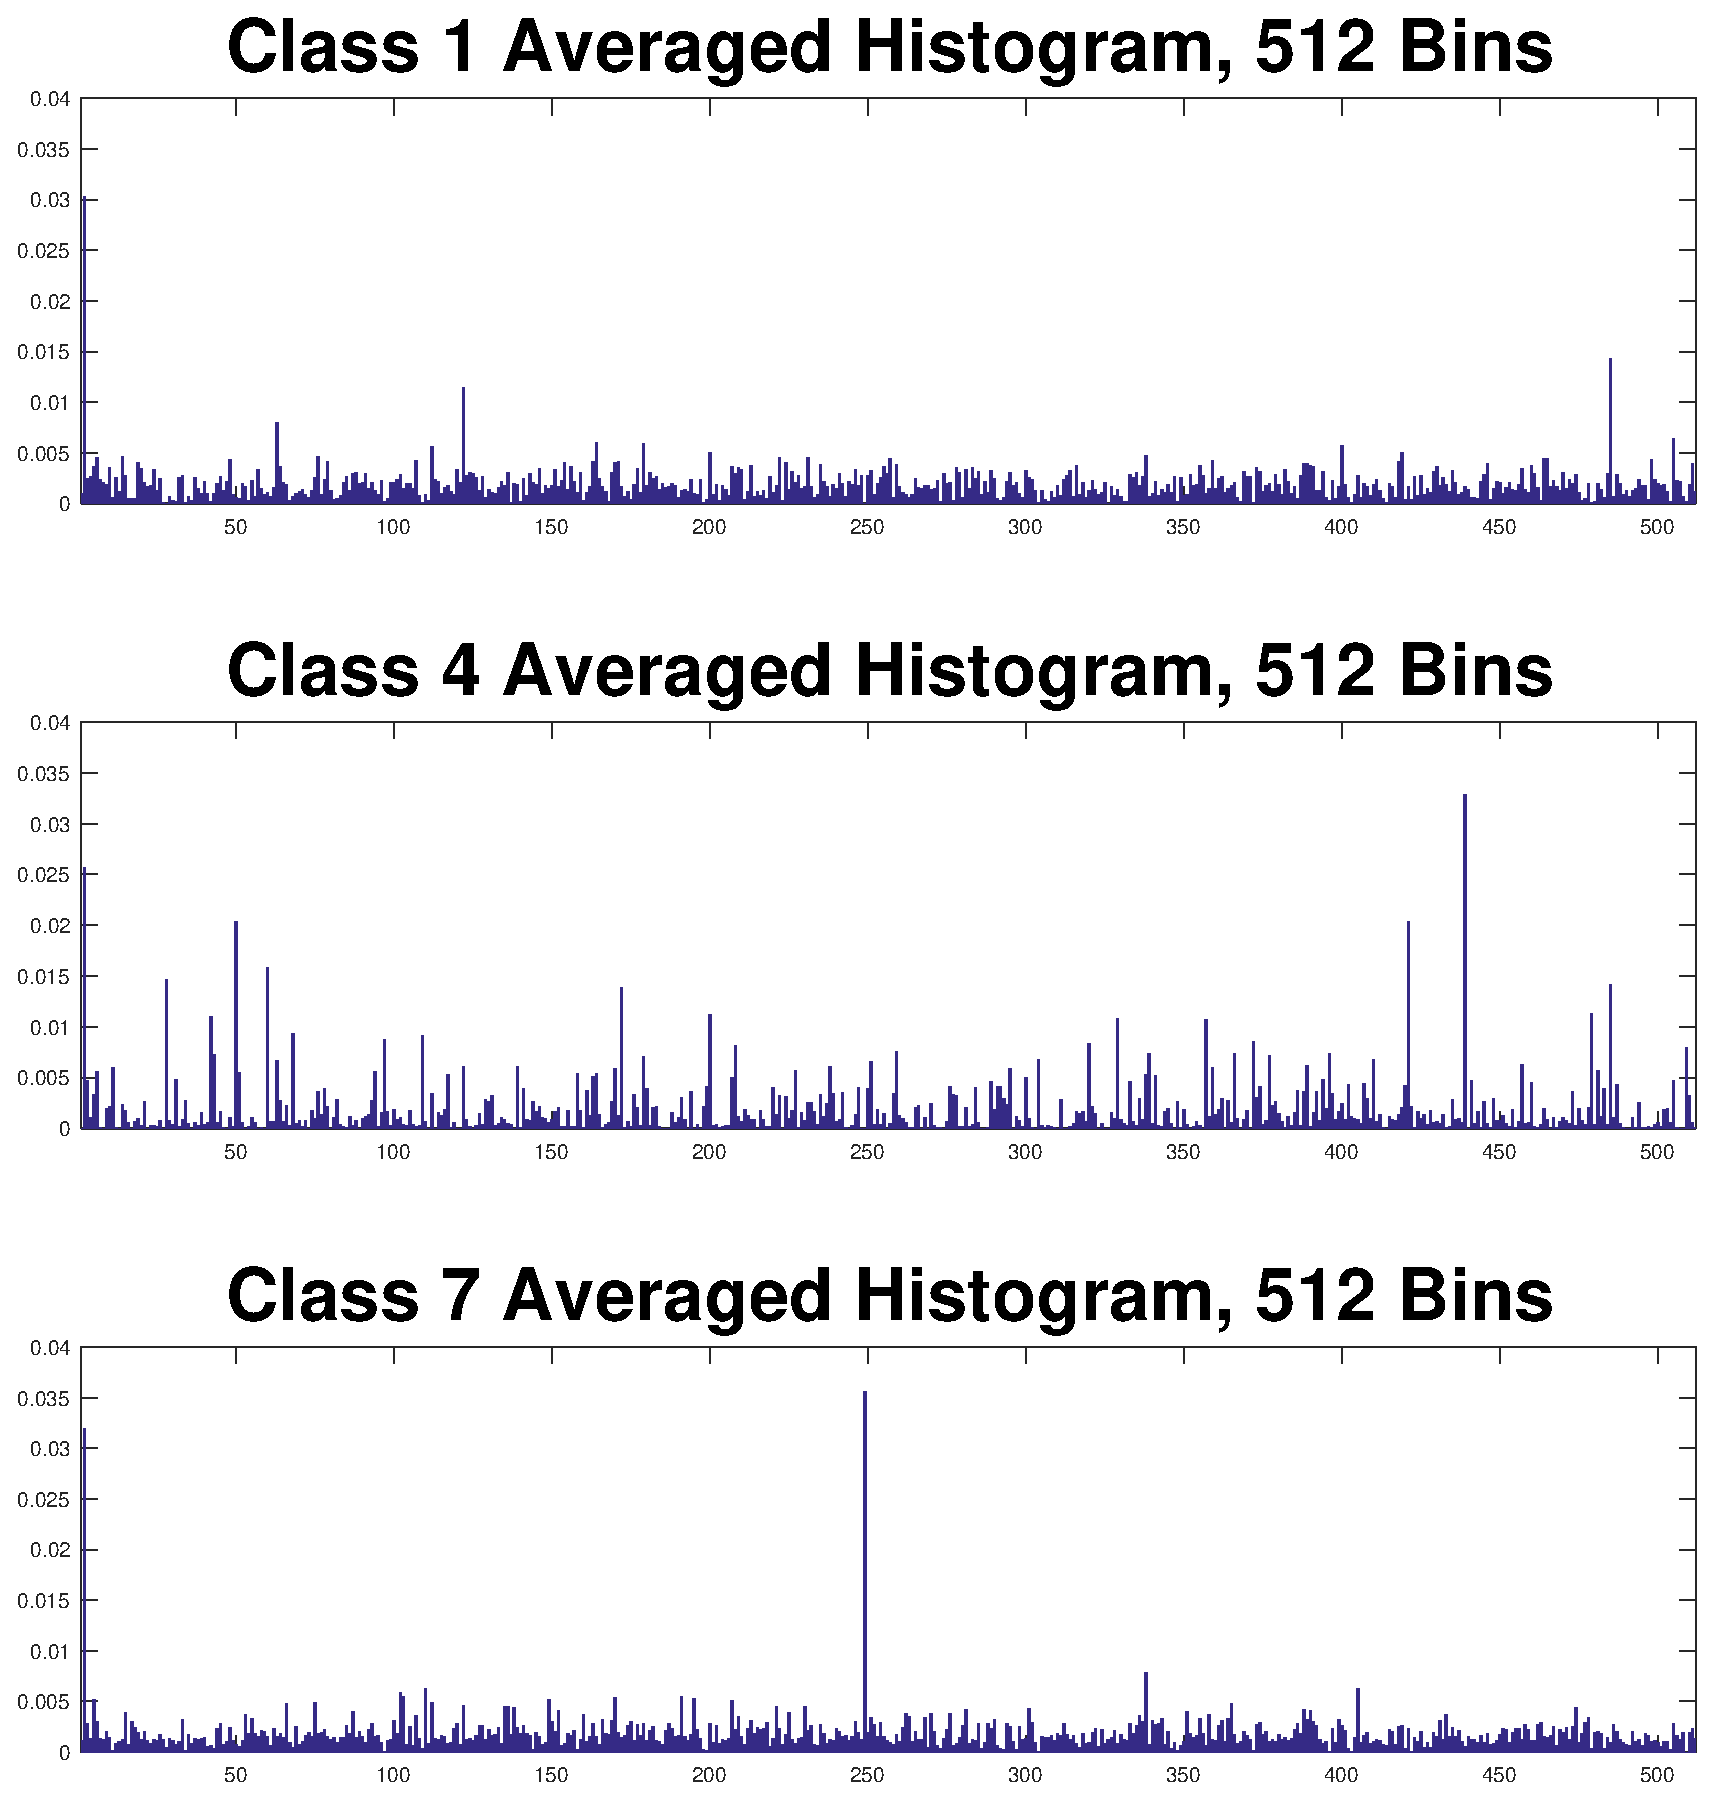
\includegraphics[width=0.49\columnwidth]{hist_512}
    \caption{Overview of spectral subtraction process}
    \label{fig:hists}
\end{figure}


The final step of the vector quantisation process is to build a BoW histogram for each image in the training dataset; for this, all of the descriptors returned by \texttt{vl\_phow} for a single image are compared to the cluster centers using matlab's inbuilt function \texttt{knnsearch}. The euclidean distance between each cluster center and each descriptor is found. The center which is closest to the descriptor in the 128-dimensional descriptor space is returned by \texttt{knnsearch}. Occurrences of each cluster center are accumulated and normalized to form a histogram. The figure below shows the averaged histograms for classes 1, 4 and 7 with the two different vocabulary sizes. 


\section{RF Classifier}

The RF classifier is trained using a histograms obtained from a codebook, consisting of 256 codewords; performance is then tested. Example successes and failures are visualized below.  Heuristic explanations can be made for some of the misclassifications that are observed. For example, the left-most watch has the characteristic 'spoty' phase transition and circular edges that are observed in wild cats. All misclassifications however cannot be explained heuristically. Two water lilies, which to the human eye are almost identical, were classified very differently. 

\begin{figure}[H]
	\centering
    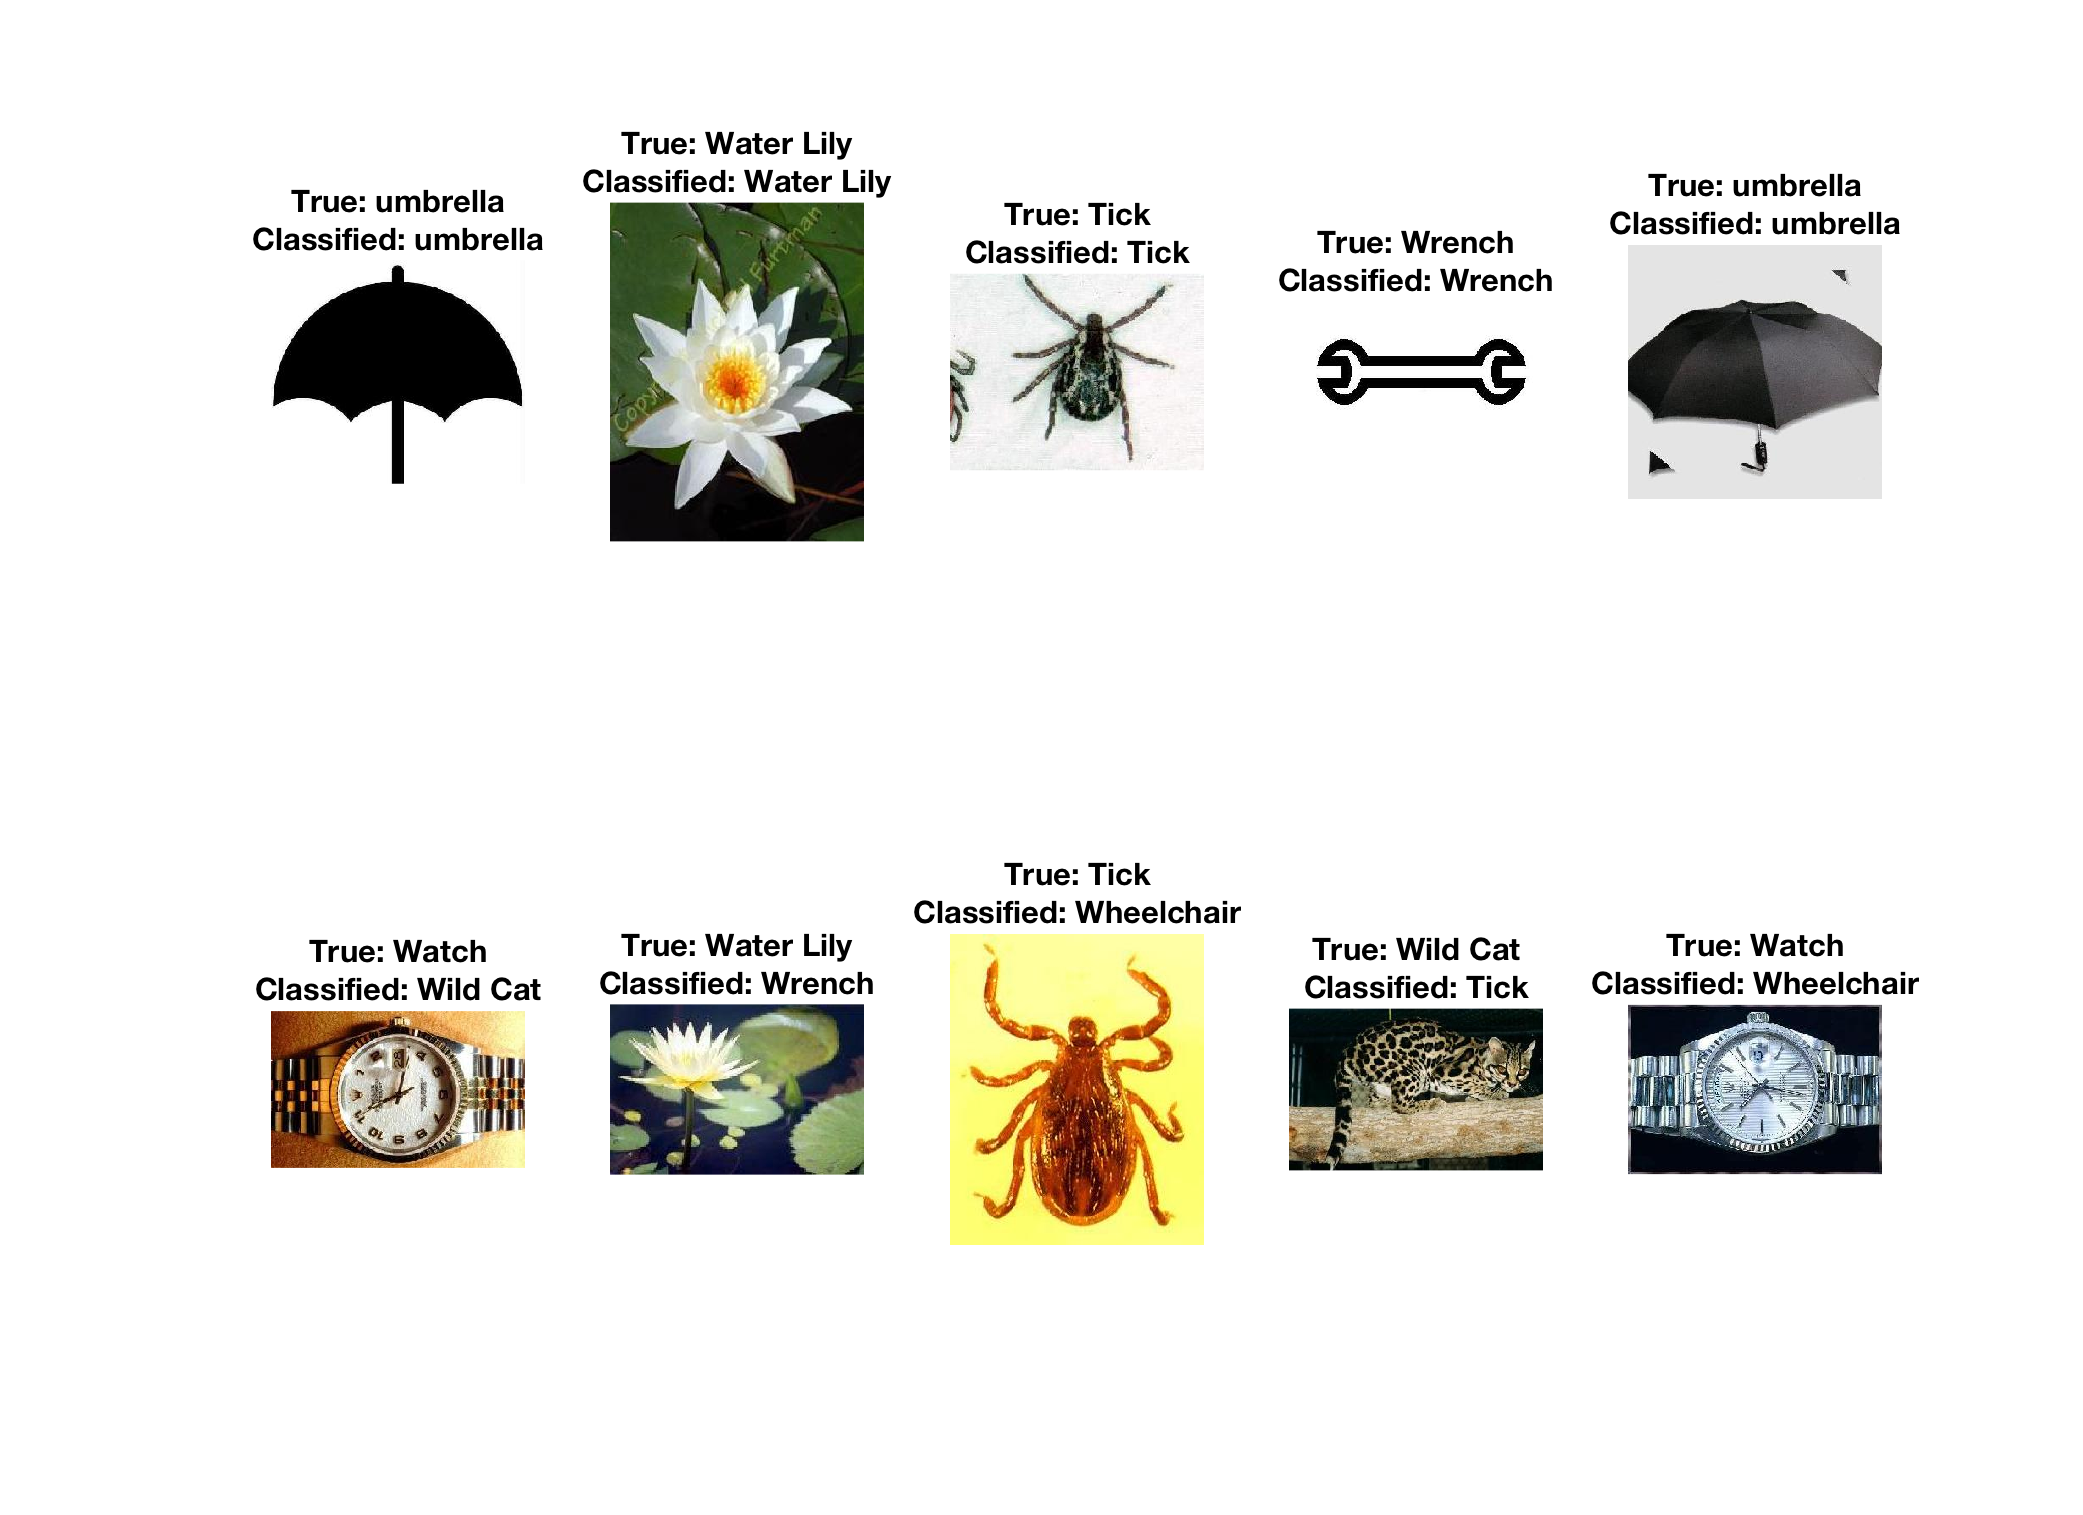
\includegraphics[width=\columnwidth]{images}
    \caption{Overview of spectral subtraction process}
\end{figure}

In general, instead of looking at individual successes and failure, the results can be summarized into a confusion matrix. The confusion matrix below shows that trilobites and windsor chair were always correctly classified, whereas the forest is the worst at identifying watches. 

\begin{figure}[H]
	\centering
    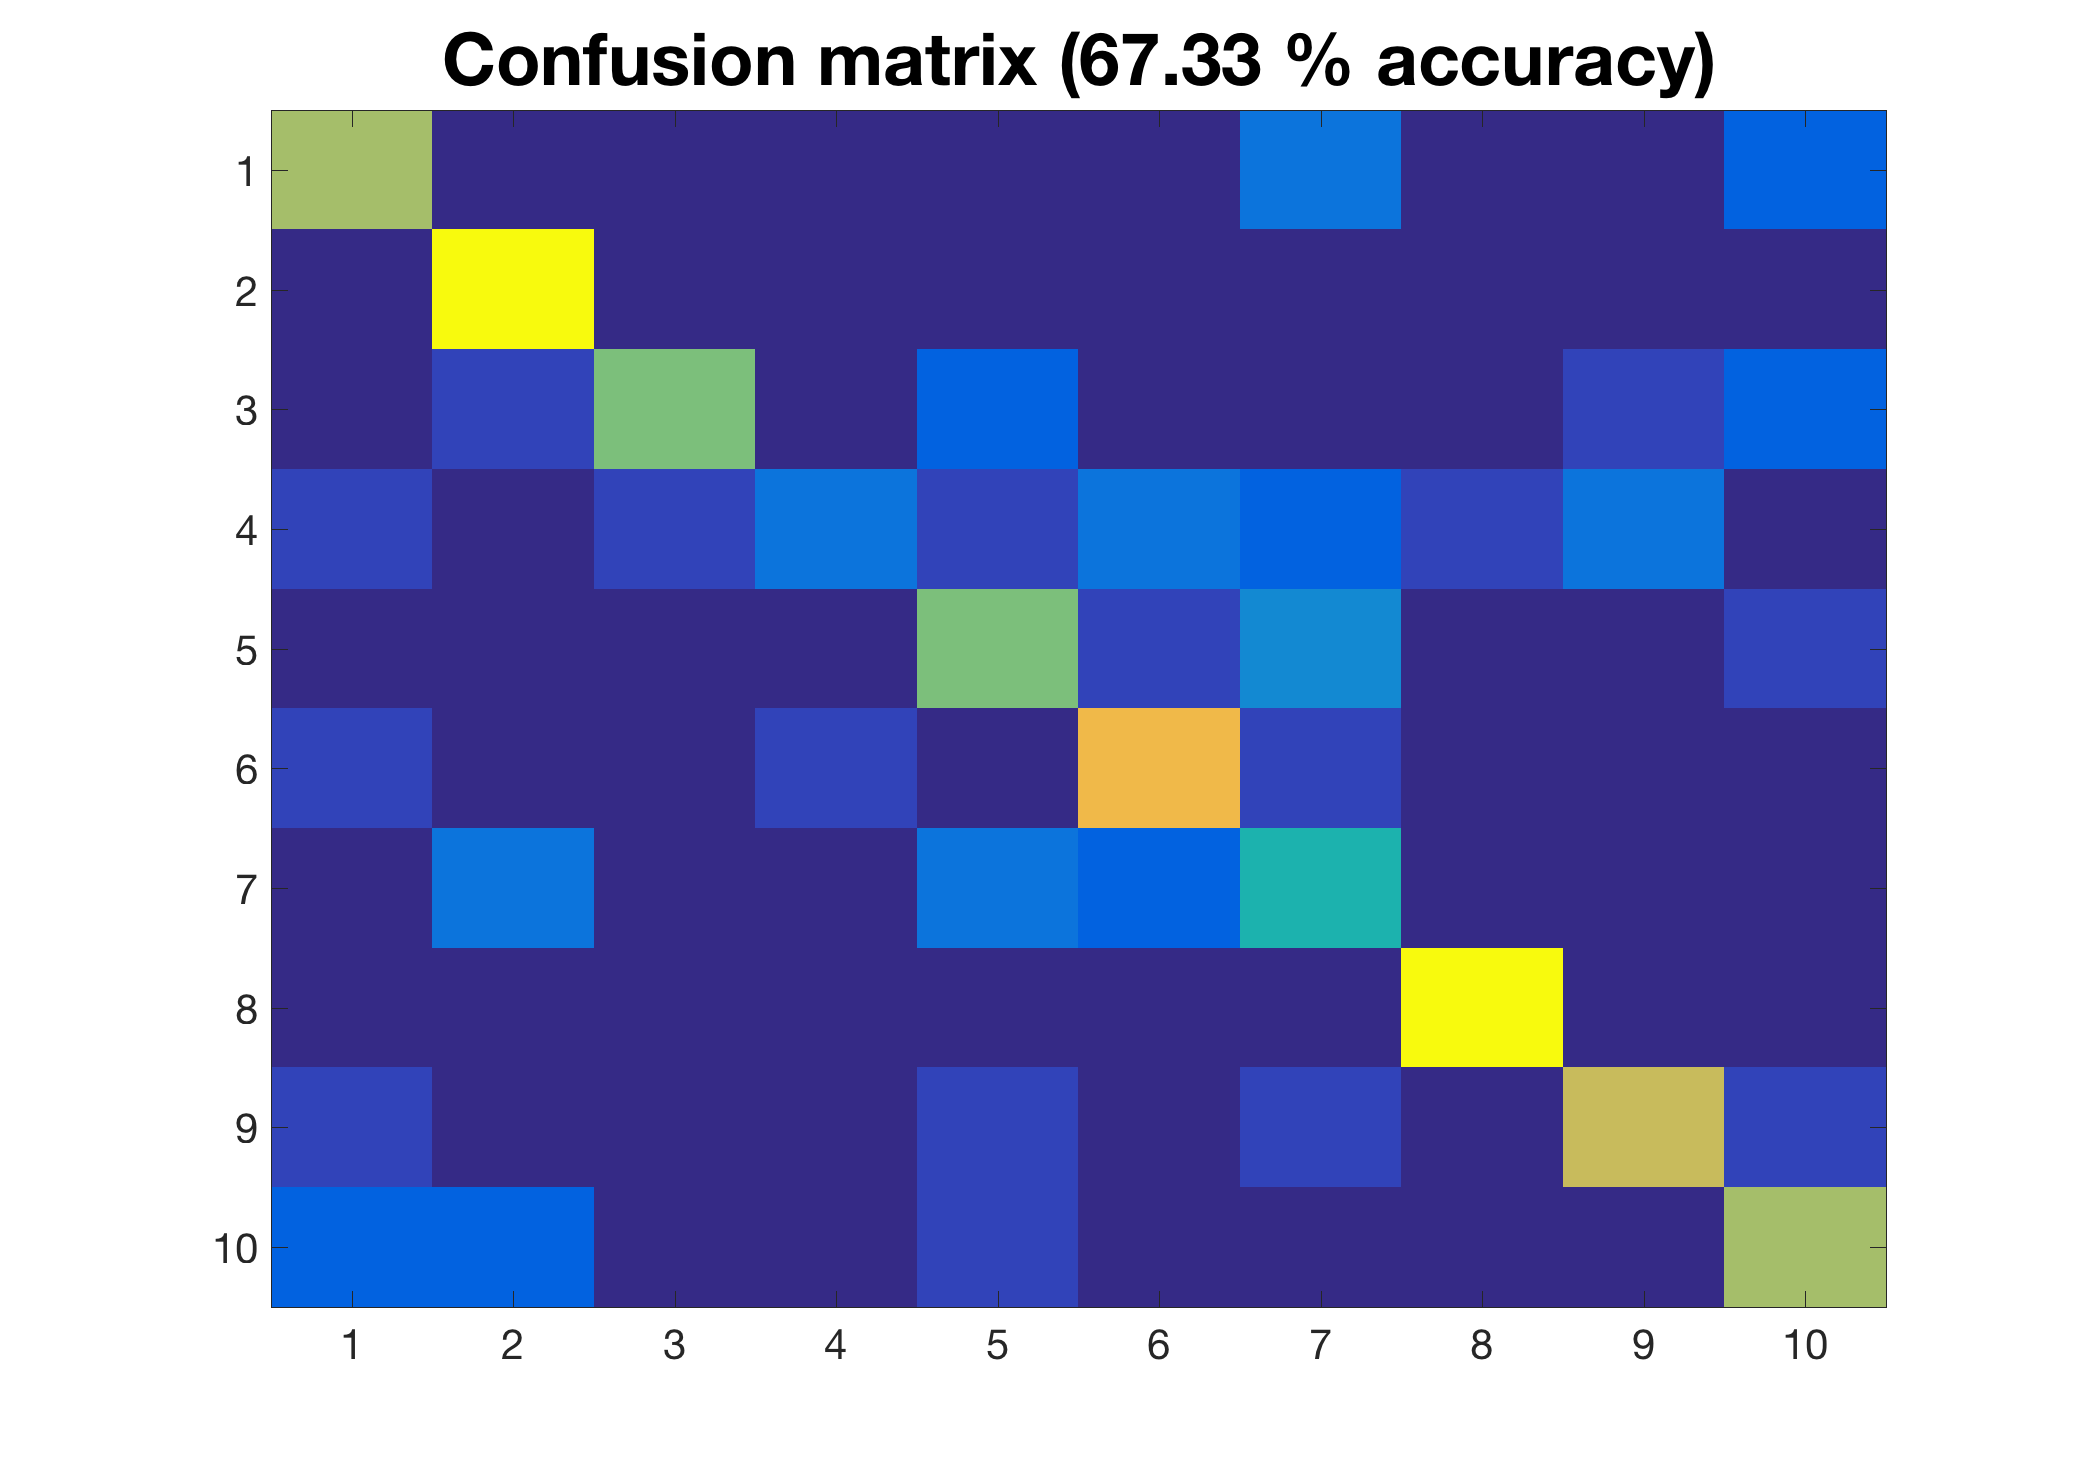
\includegraphics[width=0.70\columnwidth]{confus}    
    \caption{Overview of spectral subtraction process}
\end{figure}


\subsection*{Vocabulary Size}

Using a small vocabulary, the dimension of the space in which the RF classifier acts is small. The classes will be harder to separate in a low dimensional space. Both the numerical results in Figure \ref{fig:bins_acc} and the averaged histograms in Figure \ref{fig:hists} concretely prove that increasing the number of bins results in improved classification accuracy.

Notice however that the performance increase obtained by increasing the vocabulary size from 512 to 1024 is marginal. In fact, performance drops when an extremely large number of bins are used in conjunction with a small number of trees in the RF classifier. Although 1024 codewords gives us greater discriminating power, if the RF classifier parameters are not tuned to take into account the increase in the vocabulary size, $E_{av}$ will be high. The high error that each tree incurs can either by averaged away using the committee machine, or by increasing depth and the number of split functions tried at each node, we can lower $E_{av}$. Again, the increase in discriminating power that is associated with an increase in the number of codewords does not carry on infinitely. If the ratio of cluster centers to training points is too high, each codewords will start to lose meaning. 

As mentioned above, the K-means++ algorithm that matlab implements scales with $\mathcal{O}(\text{log} \ \text{K})$.

\begin{figure}[H]
	\centering
    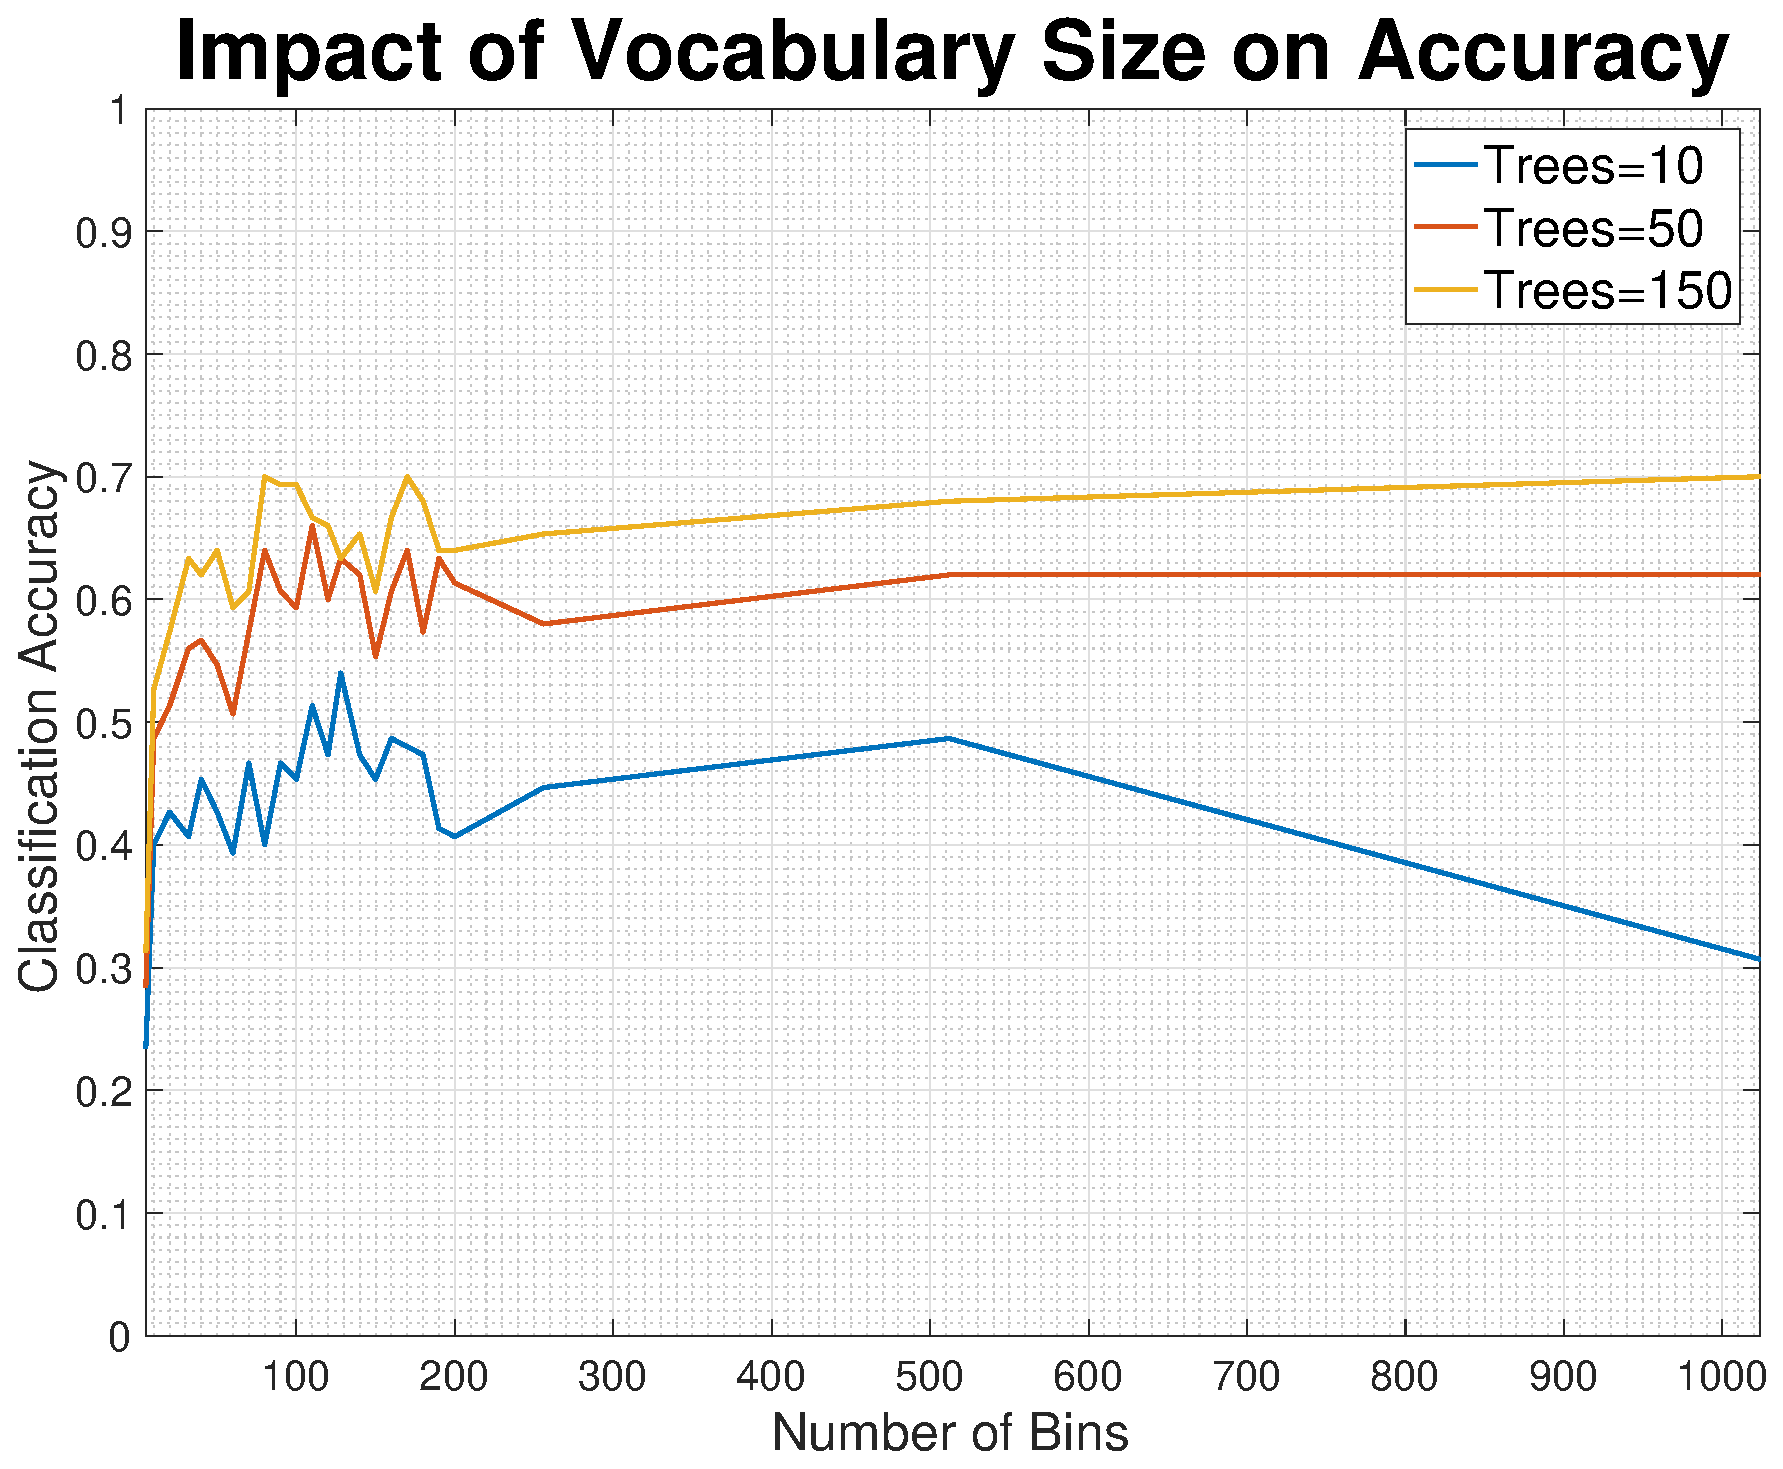
\includegraphics[width=0.49\columnwidth]{numBins_acc}
	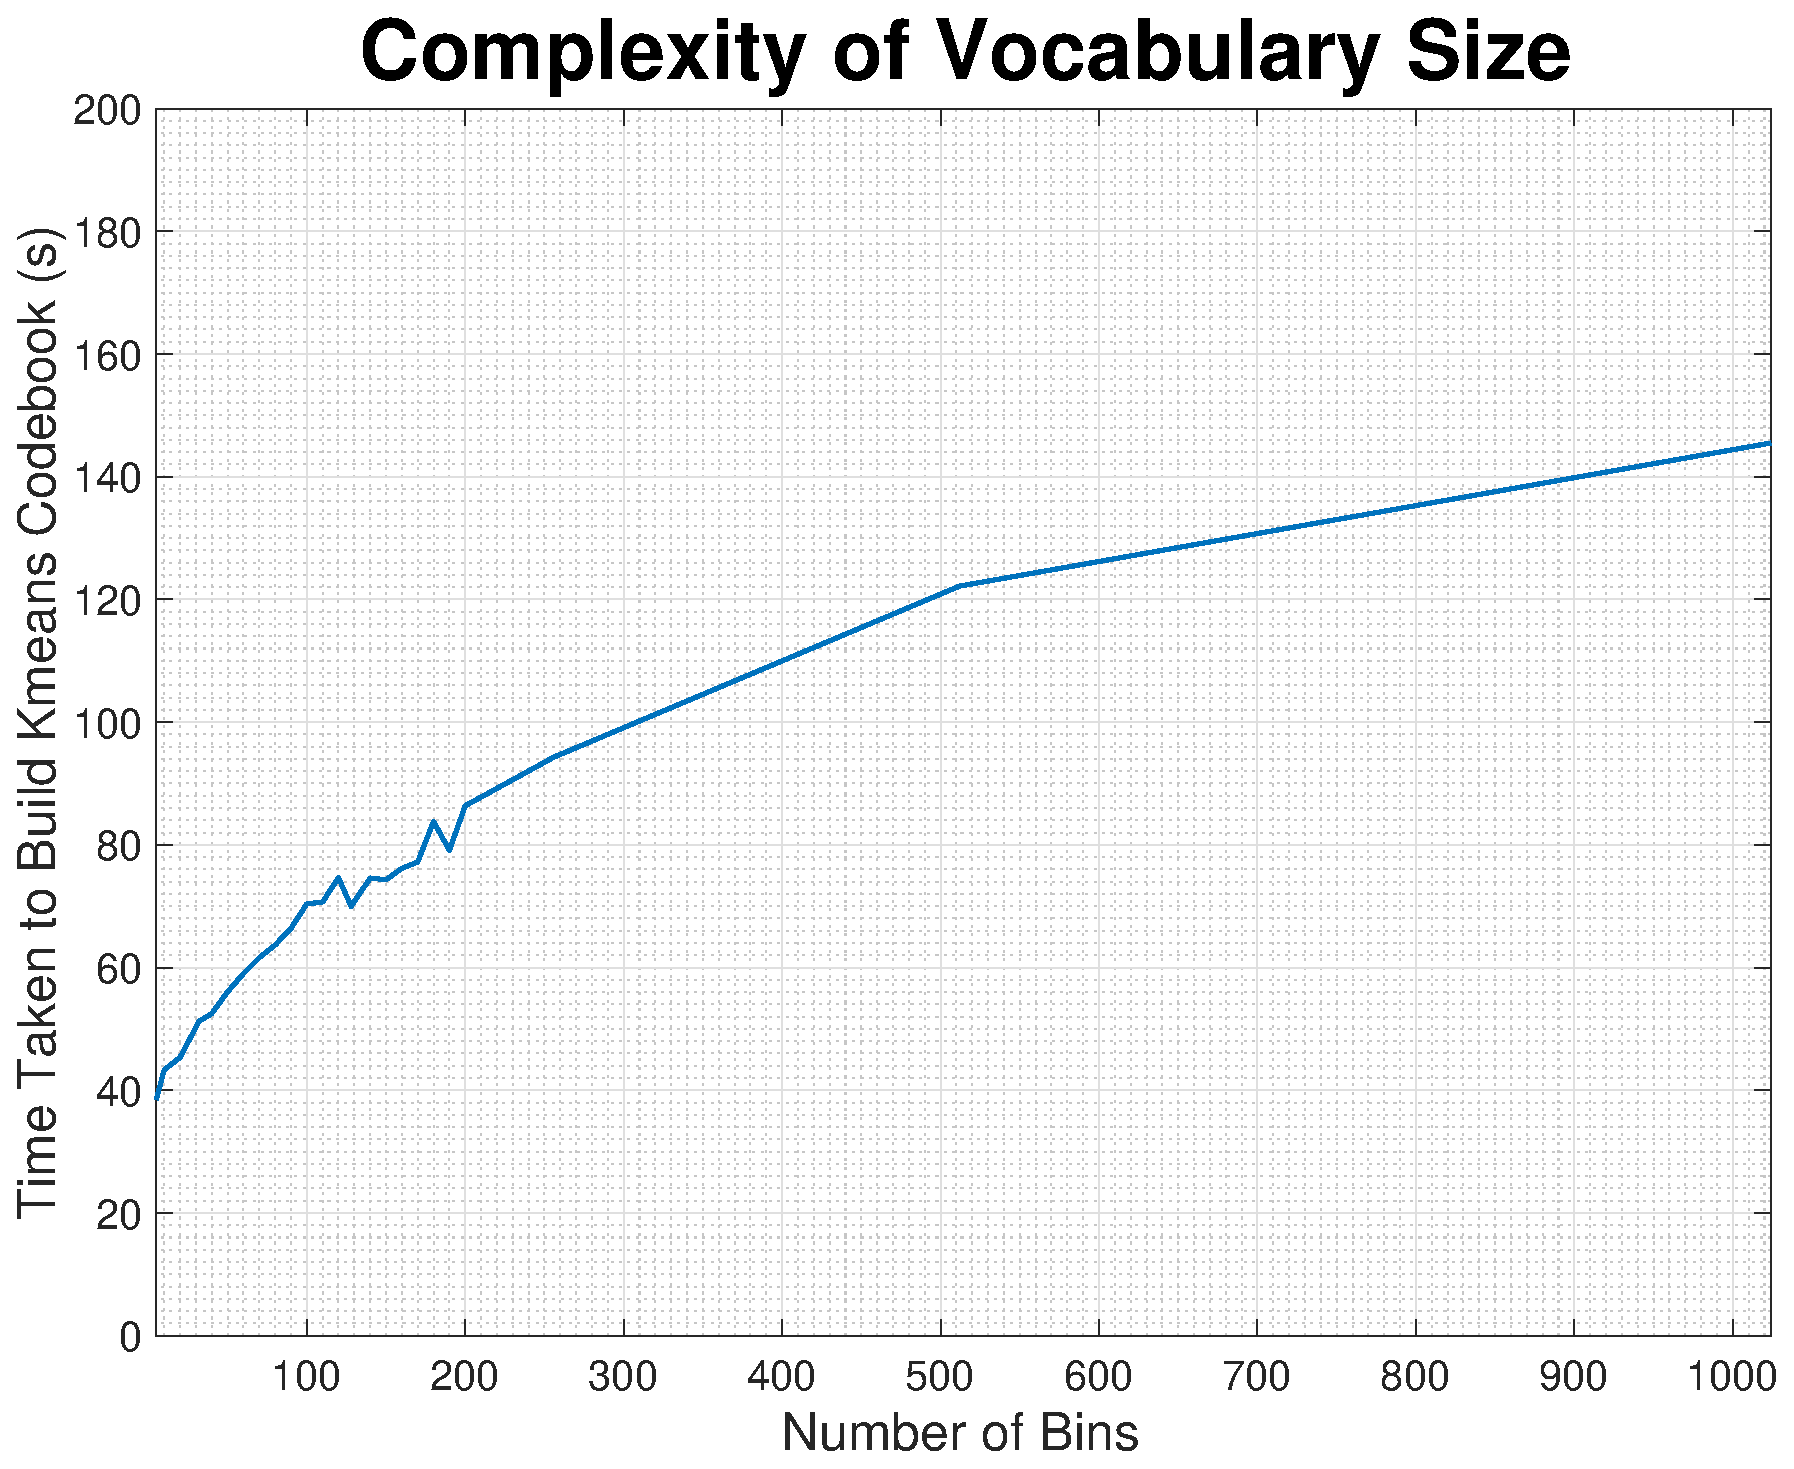
\includegraphics[width=0.49\columnwidth]{numBins_complexity}
    \caption{Overview of spectral subtraction process}
    \label{fig:bins_acc}
\end{figure}

\subsection*{Number of Trees}

The graphs below corroborate the discussion above about the effects that \texttt{numTrees} has. Regardless of the vocabulary size, increasing the number of trees yields an increase in performance. However, setting  \texttt{numTrees} to be greater that $180$ does not lead to any significant improvements in the recognition accuracy. Also, we observe that increasing the number of trees causes computational complexity to grow linearly. Note that, no parallel processing has been done as of yet; the algorithm is susceptible to parallelism. 

\begin{figure}[H]
	\centering
    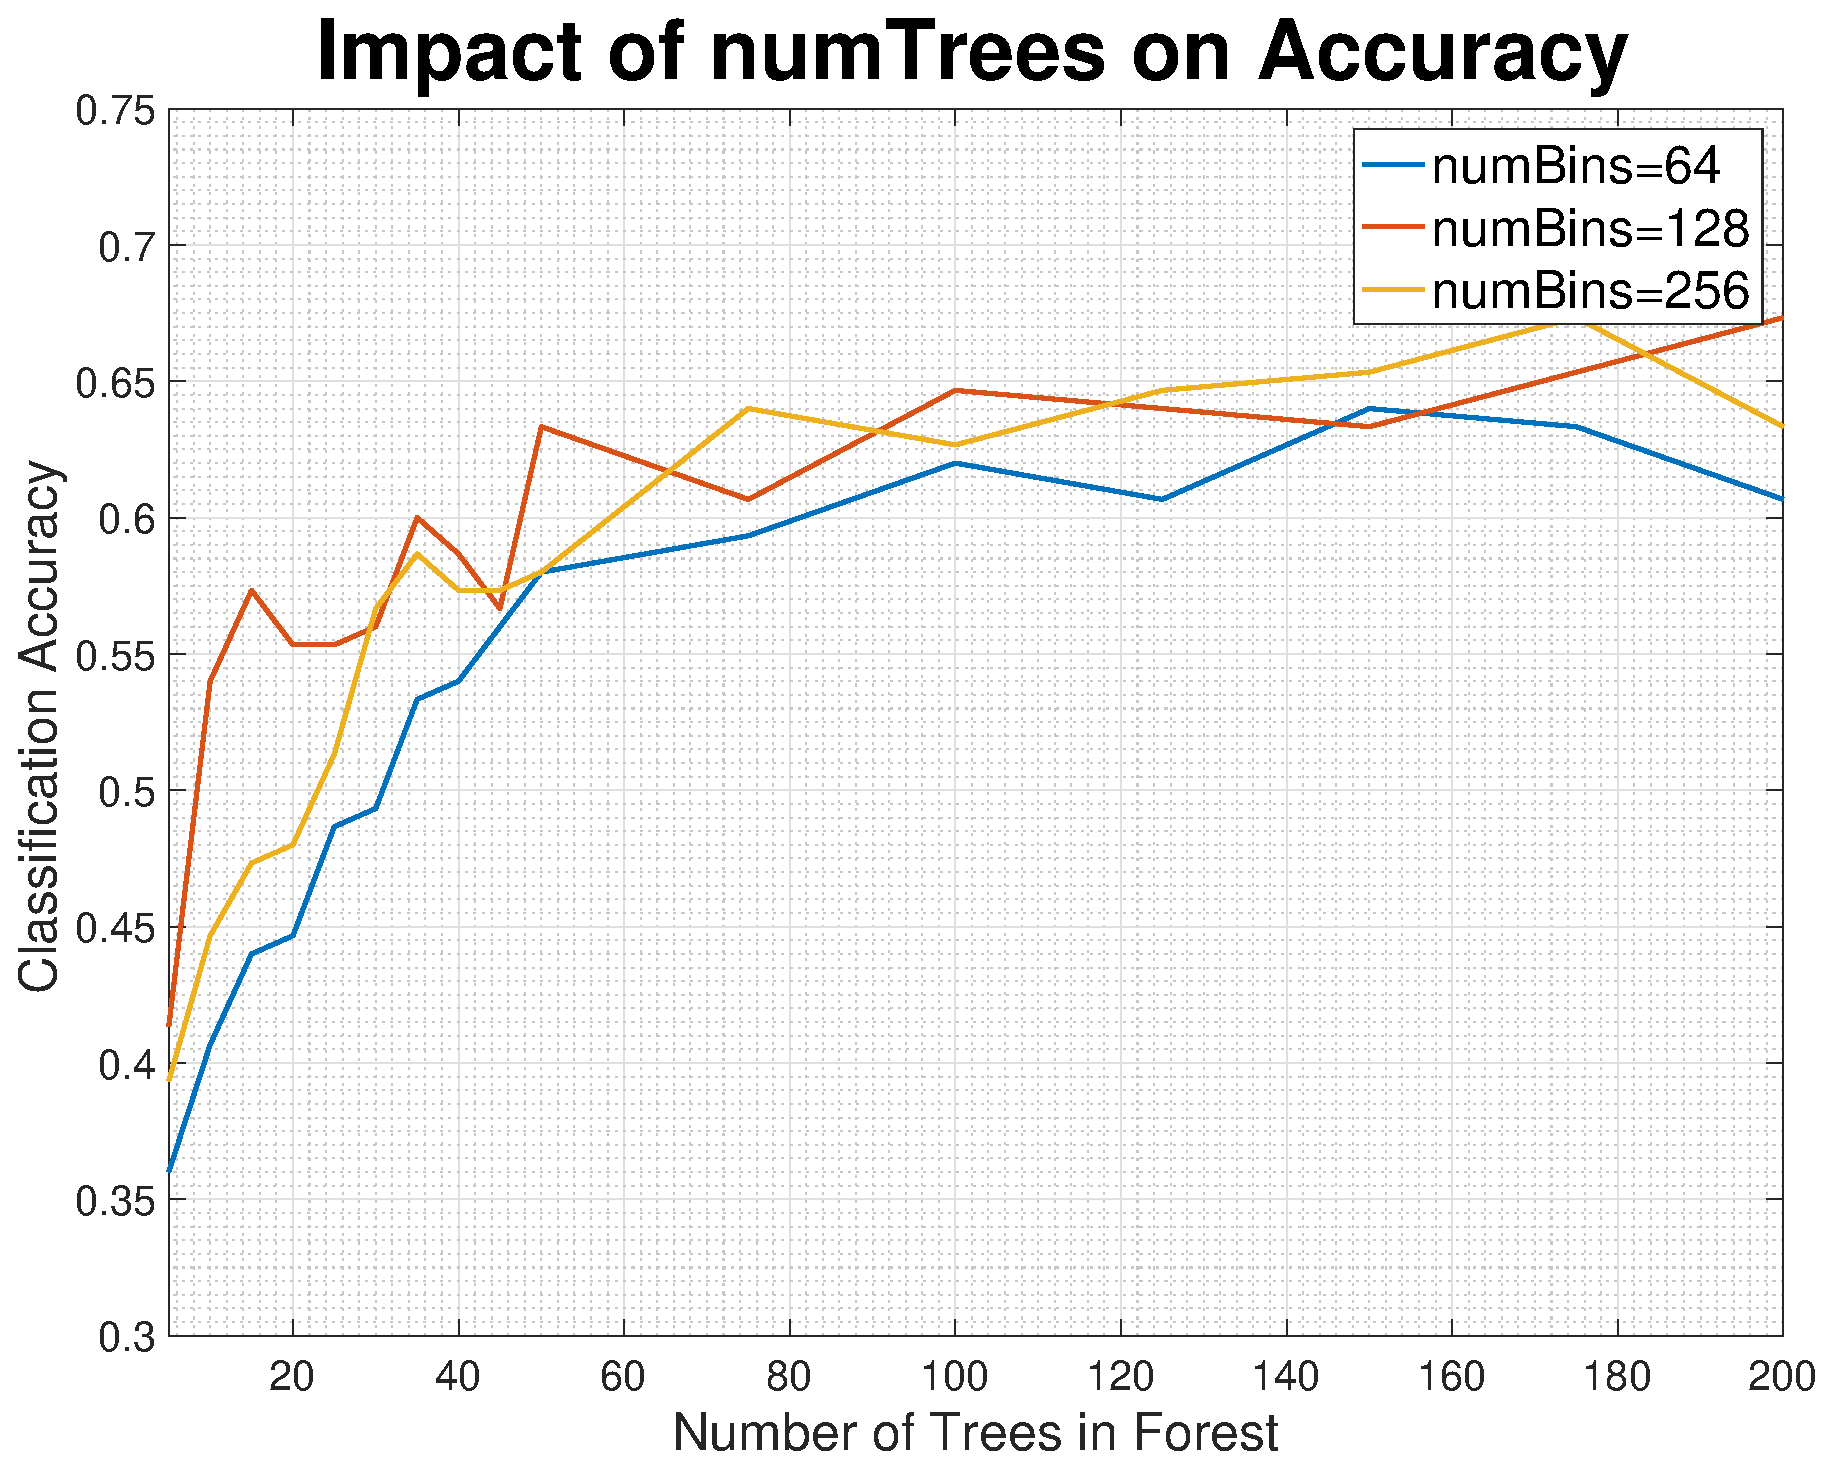
\includegraphics[width=0.49\columnwidth]{numTrees_acc}
	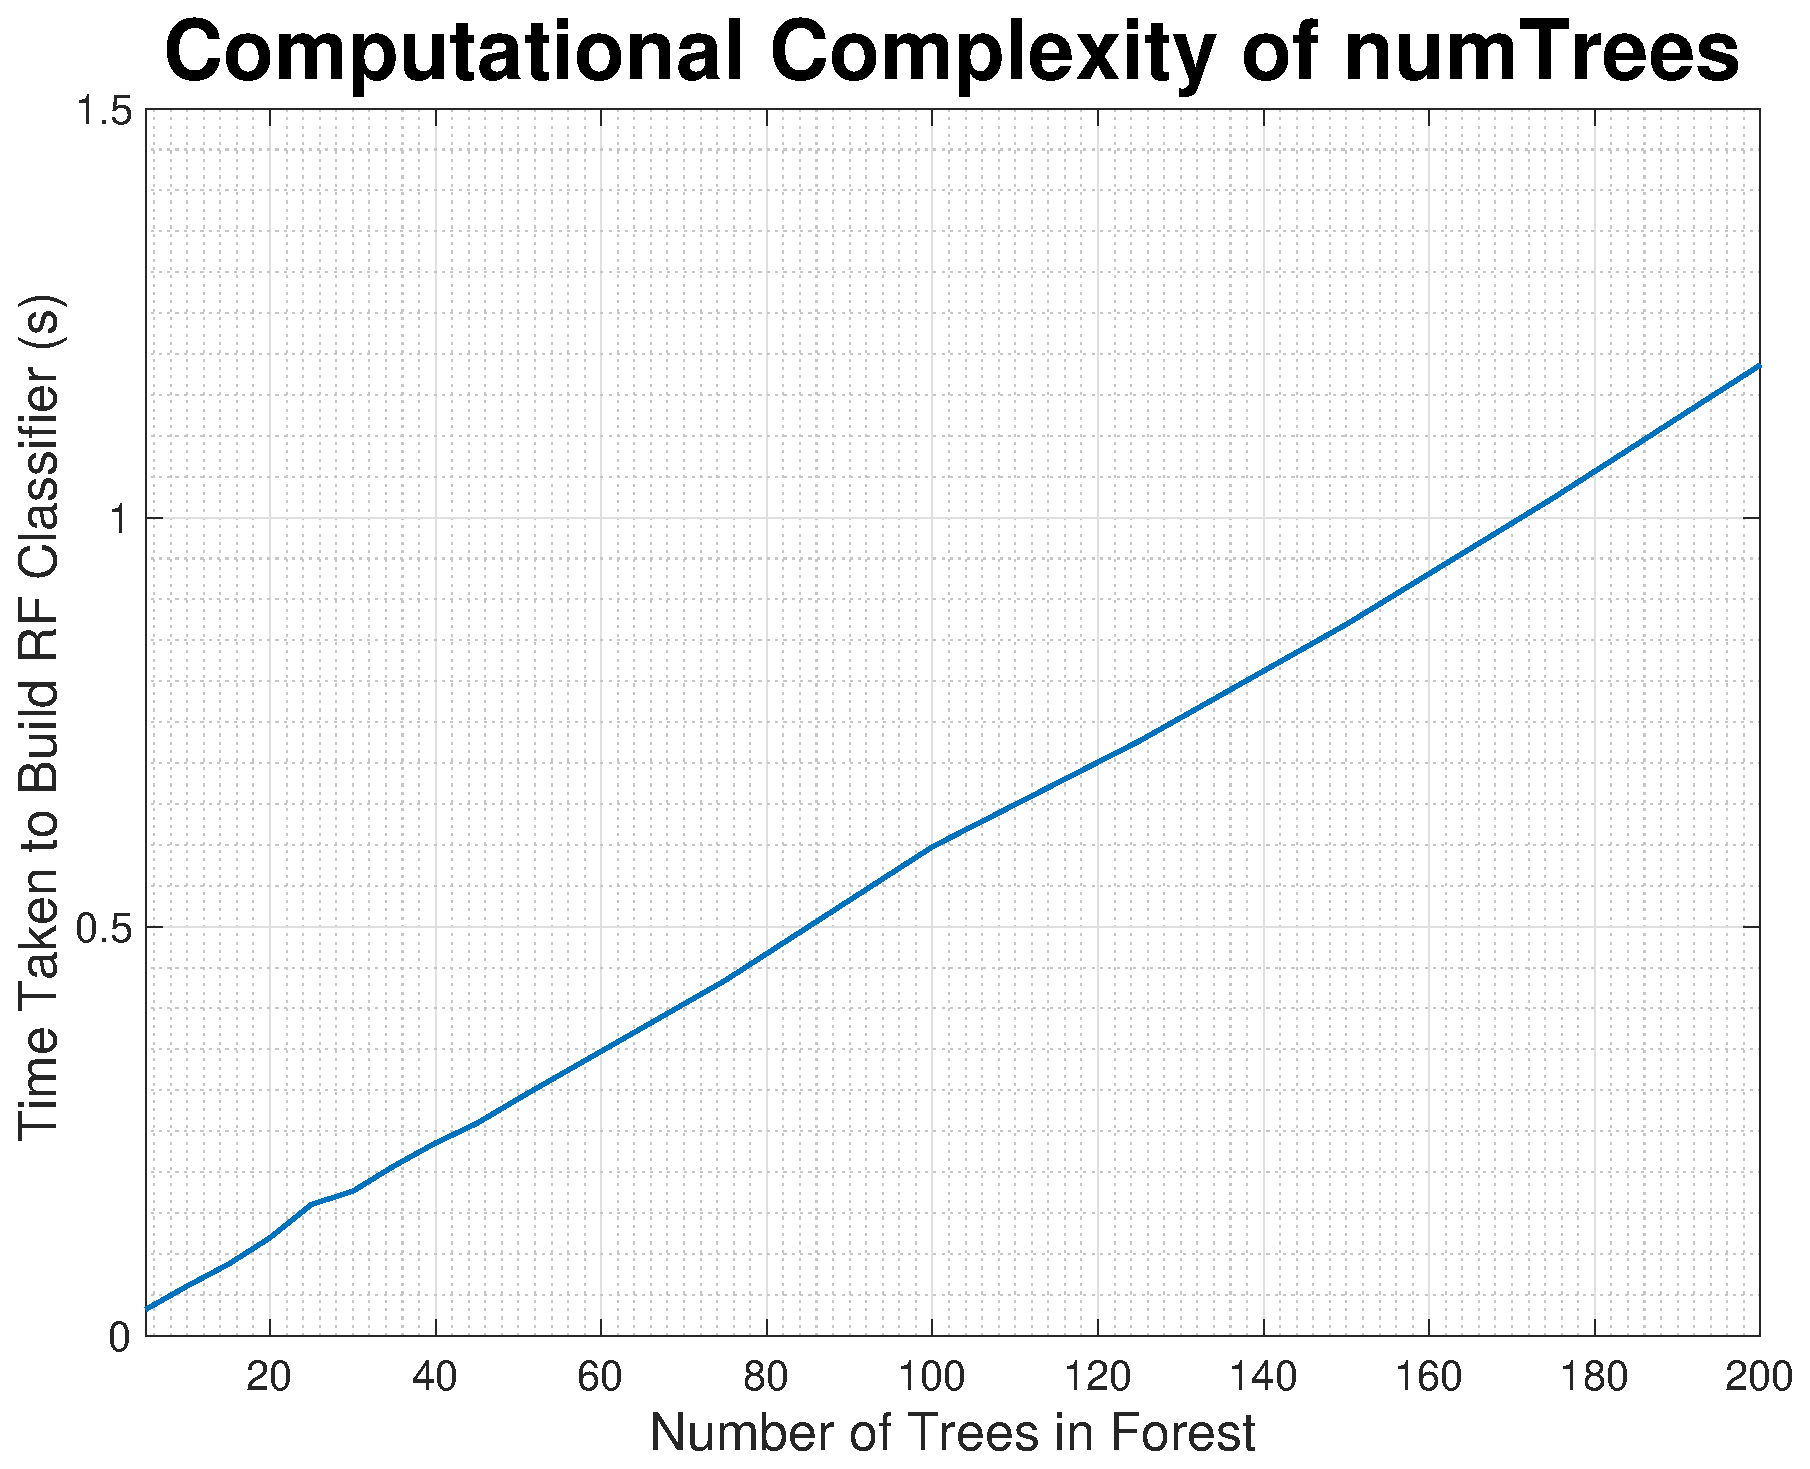
\includegraphics[width=0.49\columnwidth]{numTrees_complexity}
    \caption{Overview of spectral subtraction process}
    \label{fig:numtrees_caltech}
\end{figure}

\subsection*{Number of Split Functions}

Again, the graphs below corroborate the discussion above about the effects of increasing the number of split functions. We observed visually that setting \texttt{numSplits} to be small lead to artifacts appearing the Toy Spiral data. These artifacts are analogous to the poor recognition accuracy obtained in the figure below. We also observed that by setting \texttt{numSplits} to be extremely large, overfitting and tree interdependence would set in. Again, this is analagous to a reduction in performance after a certain point. Although the general patterns are similar, notice how different the scales are. For performance to drop, we need to set the number of split functions tested at each node to be 150. The reason for this is that instead of separating points in a 2-dimensional space as in the case of the Toy Spiral data, we are now separating points in much higher dimensions. In fact, the graphs below are obtained using a vocabulary consisting of 256 codewords. As such, to overfit the data and correlate the trees in such a large dimension, we need to try a lot of split functions. 

\begin{figure}[H]
	\centering
    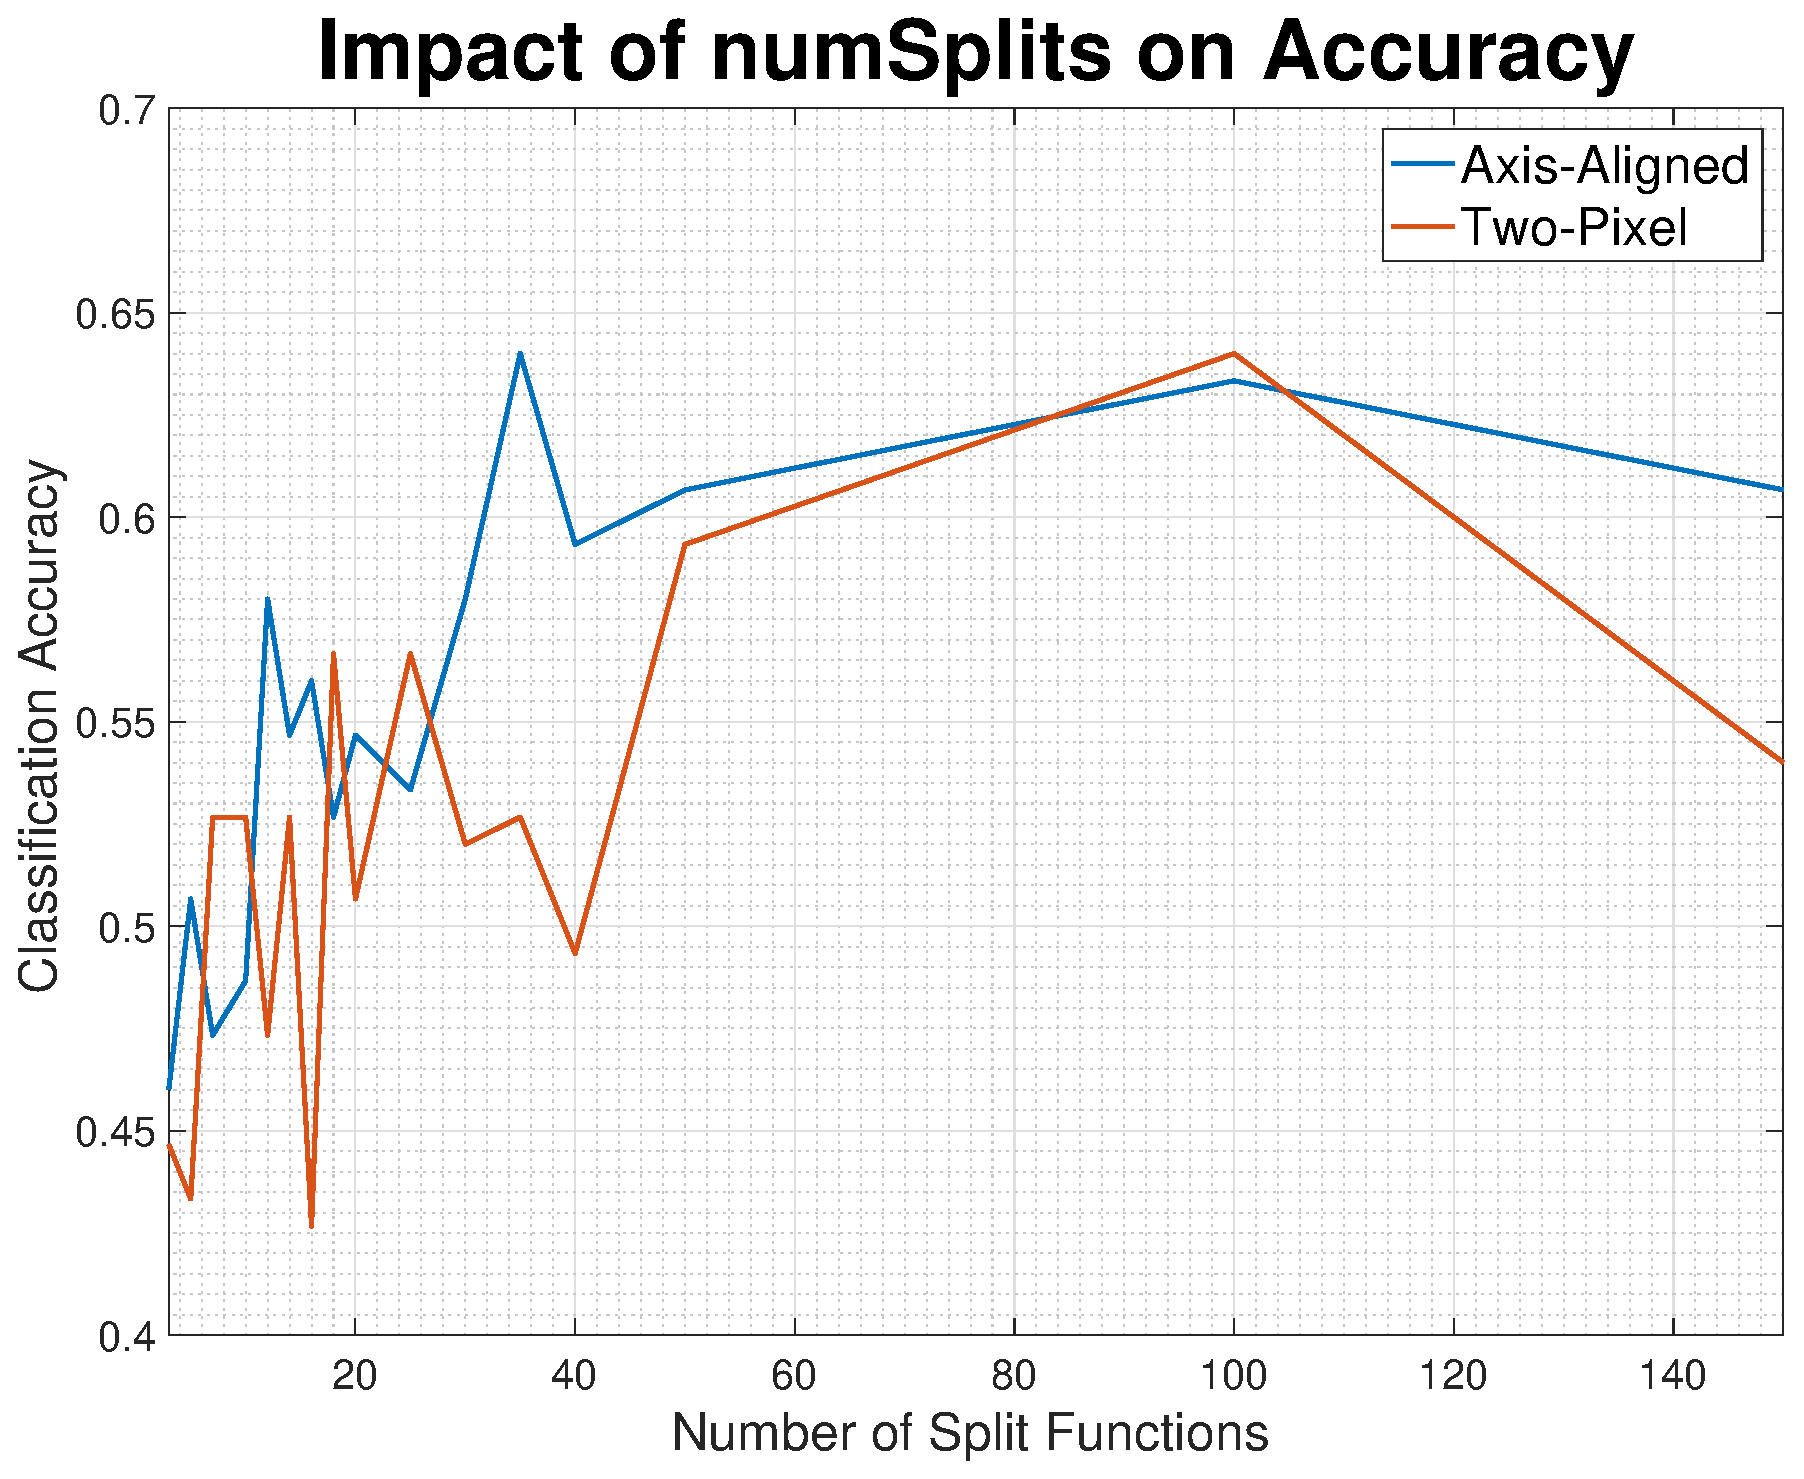
\includegraphics[width=0.49\columnwidth]{numSplits_acc}
	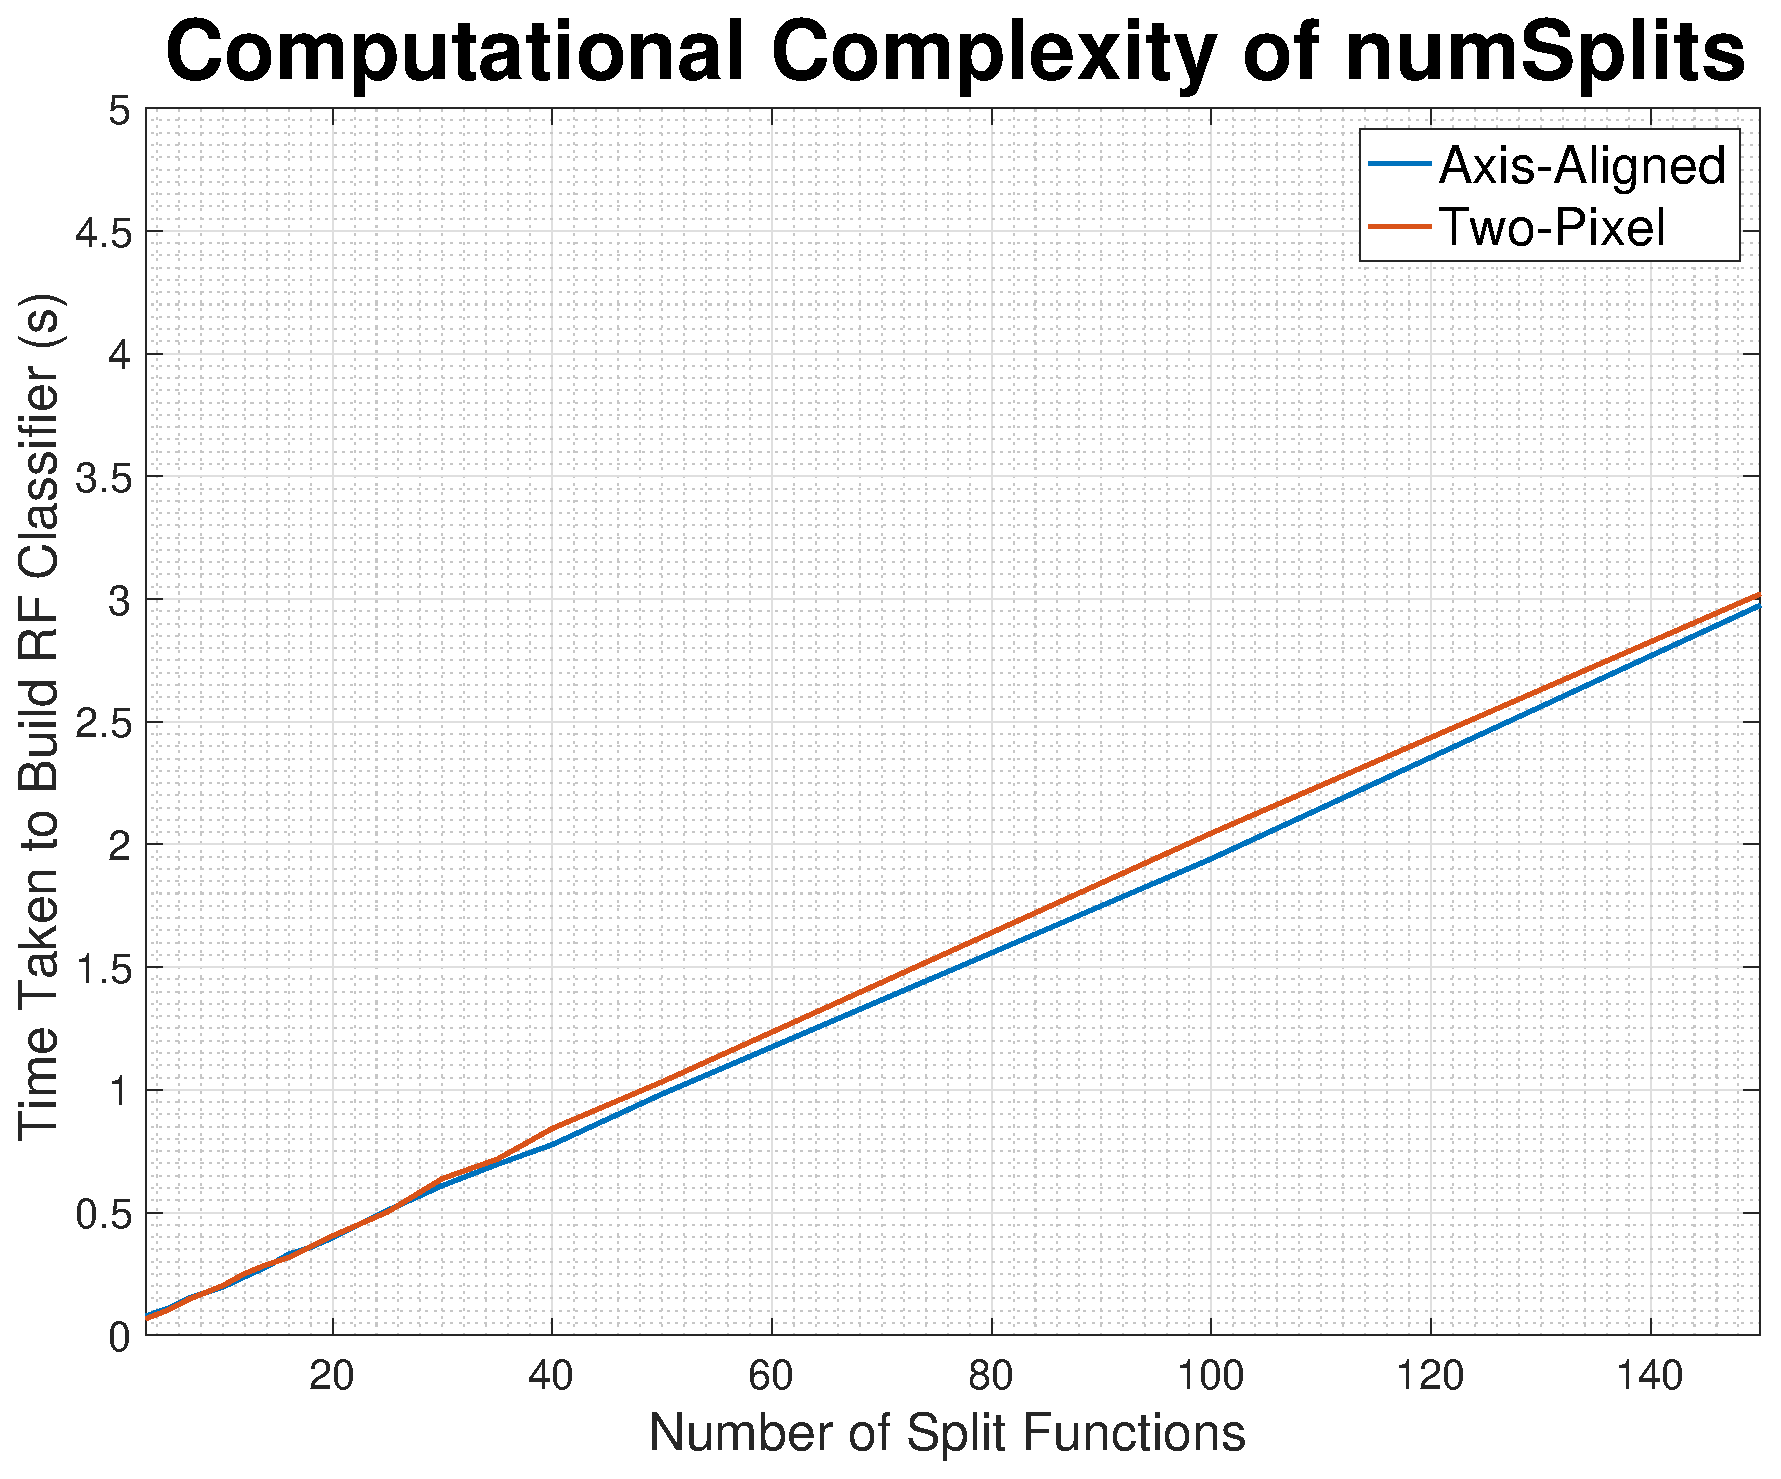
\includegraphics[width=0.49\columnwidth]{numSplits_complexity}
    \caption{Overview of spectral subtraction process}
\end{figure}

\subsection*{Depth of Tree}

Lastly, the impact of tree depth is studied. The most important thing to notice from the graphs is how poorly the algorithm scales in terms of complexity. Note that the graph shows the average time taken to grow each tree in the forest. This is expected since the number of nodes in our tree grows exponentially with tree depth. For relative good performance, we would need at least 150 trees in our forest. If each tree took $10$ seconds to grow, simply training the forest would take approximately 25 minutes. As mentioned above, increasing tree depth is not that wise and other parameters should be tuned to increase performance. Anyway, performance does not always increase with an increase in tree depth. Notice that for the axis-aligned split function, the peak performance occurs at a depth of 8. 

\begin{figure}[H]
	\centering
    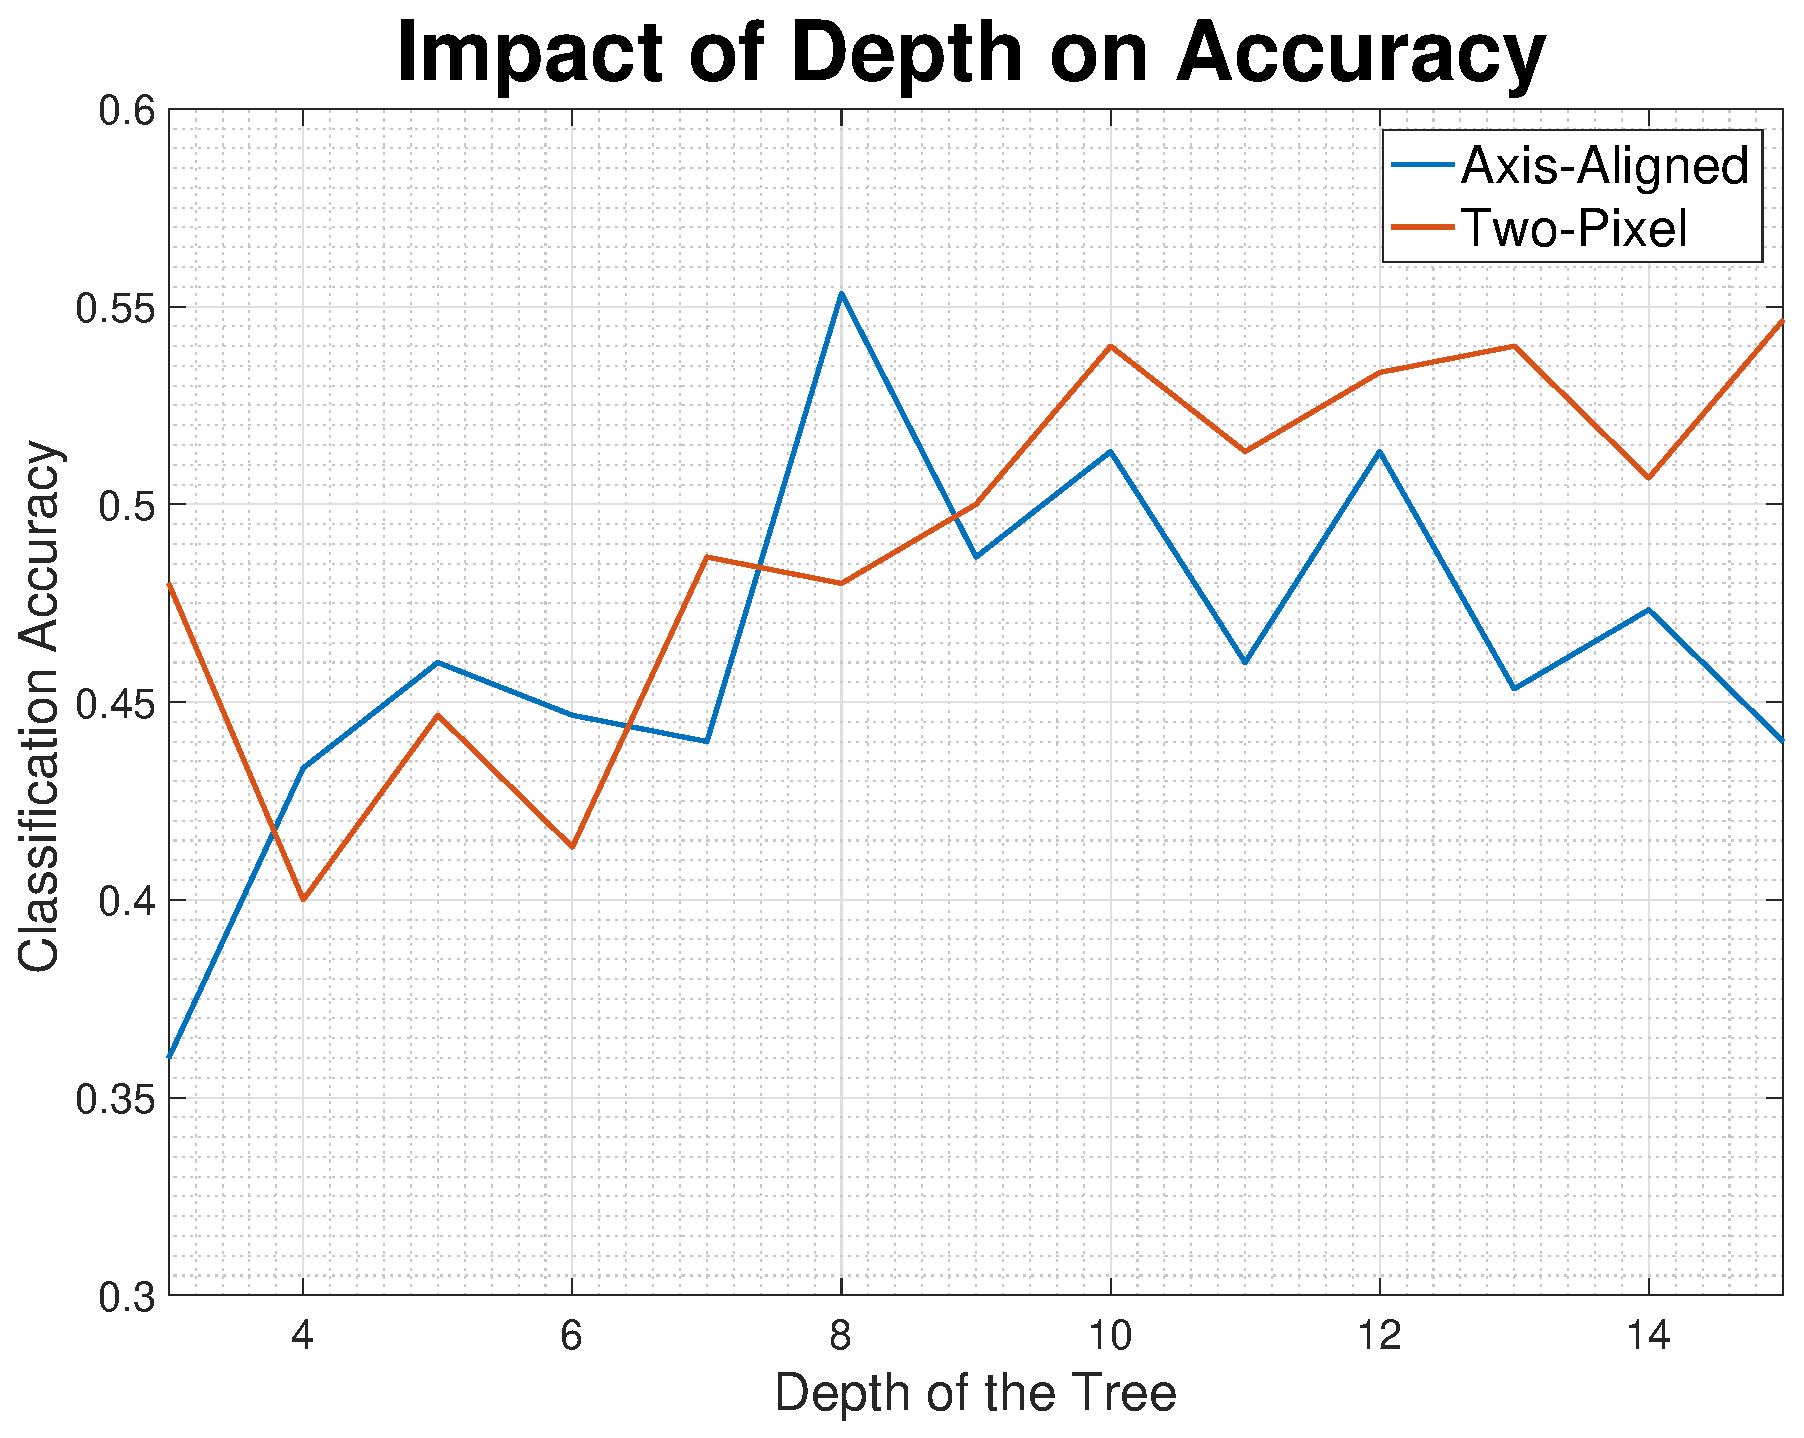
\includegraphics[width=0.49\columnwidth]{depth_acc}
	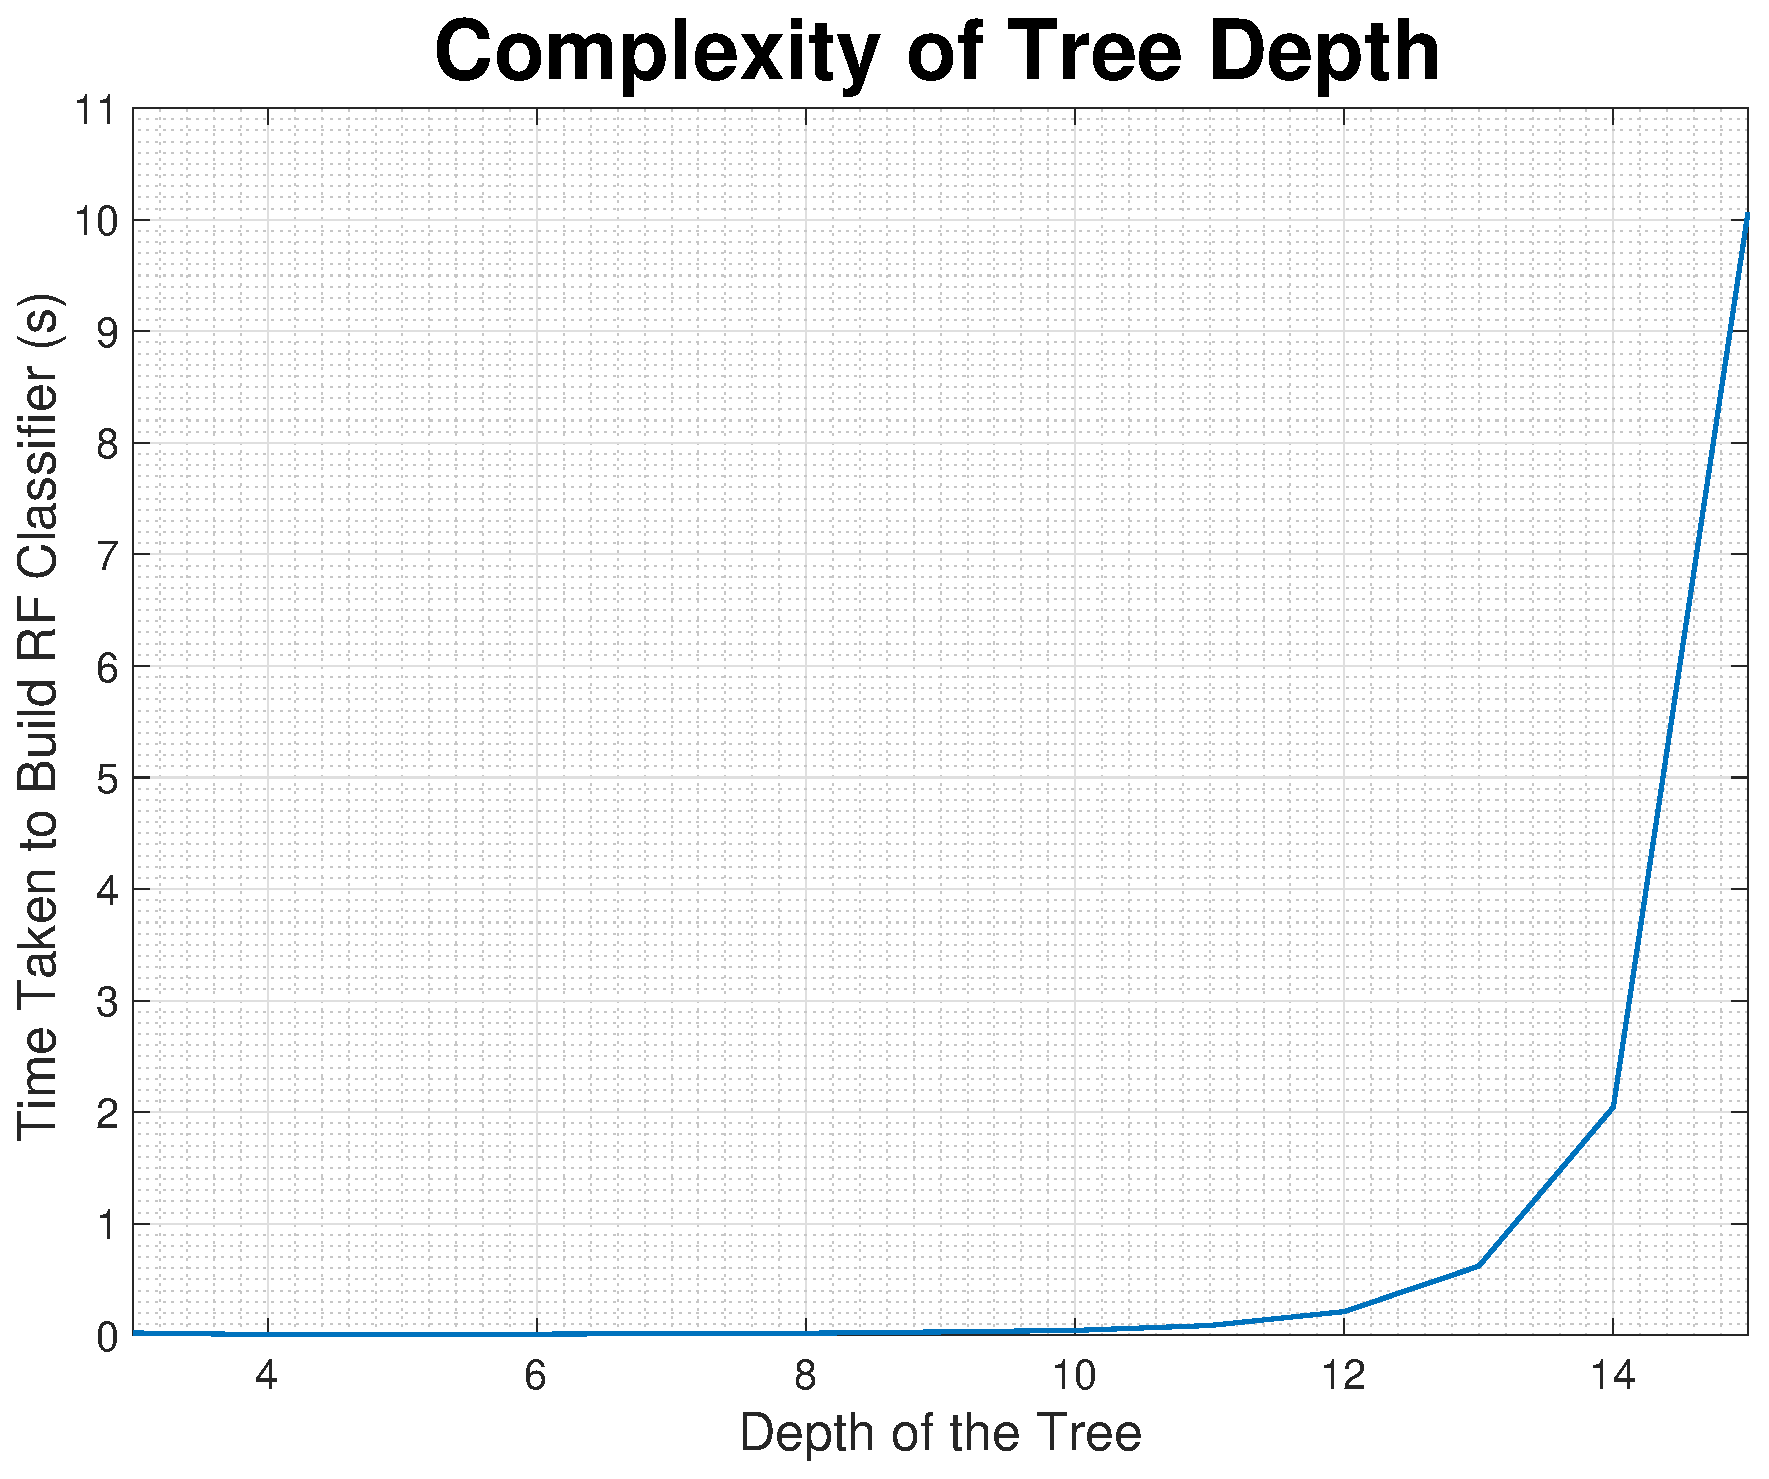
\includegraphics[width=0.49\columnwidth]{depth_complexity}
    \caption{Overview of spectral subtraction process}
\end{figure}

\section{RF Codebook}

\subsection{Overview of Codebook}

The previous section explored codebook generation using the K-means algorithm. The K-means algorithm has the advantage that it considers all 128-dimensions of the descriptor space when forming clusters. This is extremely important since the features returned by \texttt{vl\_phow} are Gaussian derivatives computed at 8 orientation planes over a $4\times 4$ grid. Using a single decision tree to generate a codebook will never return codewords with as much discriminating power as those returned by the K-means algorithm. Decision trees use weak-learners that consider a limited number of dimensions at each node. The component-wise manner in which data is filtered can never expect to produce the same results as the K-means algorithm which considers all dimensions simultaneously. However, by using an ensemble of decision trees, one can still achieve a rich and diverse codebook. RF codebooks will be analyzed in this section.

\subsection{Performance of RF Codebook}



\subsection{Computational Complexity}

As mentioned in the lecture notes, the computational complexity of the K-means algorithm is $\mathcal{O}(\text{DN}'\text{K})$ whereas the complexity of the RF codebook is $\mathcal{O}(\sqrt{\text{D}}\text{N}'\text{log K})$. In the equations, $\text{D}$ represents the dimension of the descriptor vectors, $\text{N}'$ represents the number of descriptor vectors and $\text{K}$ represents the size of the codebook. The $\text{log \ K}$ complexity with respect to the size of the codebook is the main advantage of using a RF codebook. Keeping D and N constant, the graph below shows computational complexity with respect to the number of codewords.


\section{Conclusion}

All in all, this report explores the Random Decision Forests and the explores the effect that the multiple tuning parameters have on the algorithm's accuracy. To start,multiple weak-learners were explored in section \ref{sec:train}. The discriminating power of different learning classes as well as the relation to the number of split functions over which optimization is performed was studied. With the 2-dimensional Toy Spiral dataset, artifacts due to underfitting and overfitting were visualized in section \ref{eq:eval}. Next, codebook generation using the K-means algorithm was studied. The process of generating an intermediate descriptor vector space using \texttt{vl\_phow} was briefly discussed. Next, the effect of RF tuning parameters was analyzed analytically using the CalTech 101 dataset. Conclusions such as increasing the number of trees in the forest eventually leads to a plateau and the depth of the tree causes a exponential increase in complexity were drawn and substantiated with empirical evidence. Lastly, the RF codebook was analyzed. The difficulty in generating a rich and diverse codebook due to the influence of many tune manager
\end{document}
